\chapter{Исследование суб- и мезомасштабной динамики океана по оптическим и радиолокационным изображениям} \label{chap:3}



В предыдущих главах была описана модель формирования изображения морской поверхности в области солнечного блика и применена к анализу оптических данных MODIS и MERIS. ЕЕсли вариации СКН проявляются в блике, можно предположить, что трансформация спектра ветровых волн и, связанных с ним СКН, на течениях произвольной природы так же должно позволять наблюдать динамику океана на изображениях солнечного блика. В этой главе рассматриваются примеры исследования суб- и мезомасштабной динамики Океана по данным спутниковых оптических и радиолокационных сенсоров.



\section{Внутренние волны} \label{sec:3.1}


Подход тестируется на ВВ -- как простейшем типе течений. В качестве примера рассматривается район западно-экваториальной Атлантики, напротив устья реки Амазонки, который является областью регулярного возникновения очень мощных внутренних волн (ВВ), формируемых полусуточными приливными волнами (см. например, \citep{Ivanov1993}). Экспериментальные исследования ВВ и их влияния на обрушения ветровых волн, проведенные в этом районе, представлены в работе \citep{1986}. В этих экспериментах было обнаружено, что интенсивность ВВ коррелировала с фазами Луны, т.е. генерация ВВ имела явно приливное происхождение. В периоды интенсификации ВВ, амплитуды ВВ достигали 100\textit{м}, а при прохождении ВВ (в направлении на Северо-восток, противоположному ветру) на поверхности возникали коррелированные со смещениями термоклина области сильной интенсификации обрушения ветровых волн. Усиление обрушения (в несколько раз по отношению к фоновым значениям) возникало при заглублении термоклина, и почти исчезало при поднятии термоклина, т.е. усиление/подавление обрушения ветровых волн происходило в зонах конвергенции/дивергенции течений индуцированных ВВ на морской поверхности. 

Исходное изображение MODIS/Aqua этого района, полученное 26 апреля 2009, 16:20 показано на Рисунке~\ref{fig:3.1a}.

Несмотря на то, что наблюдаемая область частично покрыта облаками, на снимке легко различимы солнечный блик и линейчатые вариации яркости внутри блика (поверхностные проявления ВВ). Также, на Рисунке~\ref{fig:3.1} приводятся поля относительных вариаций яркости $\widetilde{B}/\overline{B}$ (Рисунок~\ref{fig:3.1b}) и передаточная функция $T$ (Рисунок~\ref{fig:3.1c}). Очевидно, что поле относительных вариаций яркости уже содержит признаки ВВ в солнечном блике. Но, в отличие от примера с нефтяным разливом в Мексиканском заливе, в данном случае передаточная функция не имеет зоны инверсии контрастов. Поэтому, как следует из уравнения \eqref{eq:1.7} знак $\widetilde{B}/\overline{B}$ противоположен знаку контрастов СКН.

На Рисунке~\ref{fig:3.1c} приводятся контрасты СКН, отражающие поверхностные проявления ВВ. Поле ВВ имеет характер чередующихся цугов ВВ, распространяющихся в северо-восточном направлении. В начале каждого из цугов идет уединенная волна (солитон).

Расстояние между ведущими солитонами в цугах примерно равно 130-150\textit{км}. Следом за ведущими солитонами распространяются пакеты более коротких ВВ с длинами волн порядка 1\textit{км}. Поскольку предполагается, что источником генерации ВВ в данном районе являются полусуточные приливные волны, по расстоянию между цугами легко оценить фазовую скорость ВВ, которая составляет примерно 3,5\textit{м/c}.



\begin{figure}[H]
   	\centering
	\begin{minipage}{.47\textwidth}
	    \subcaptionbox{\label{fig:3.1a}}
		{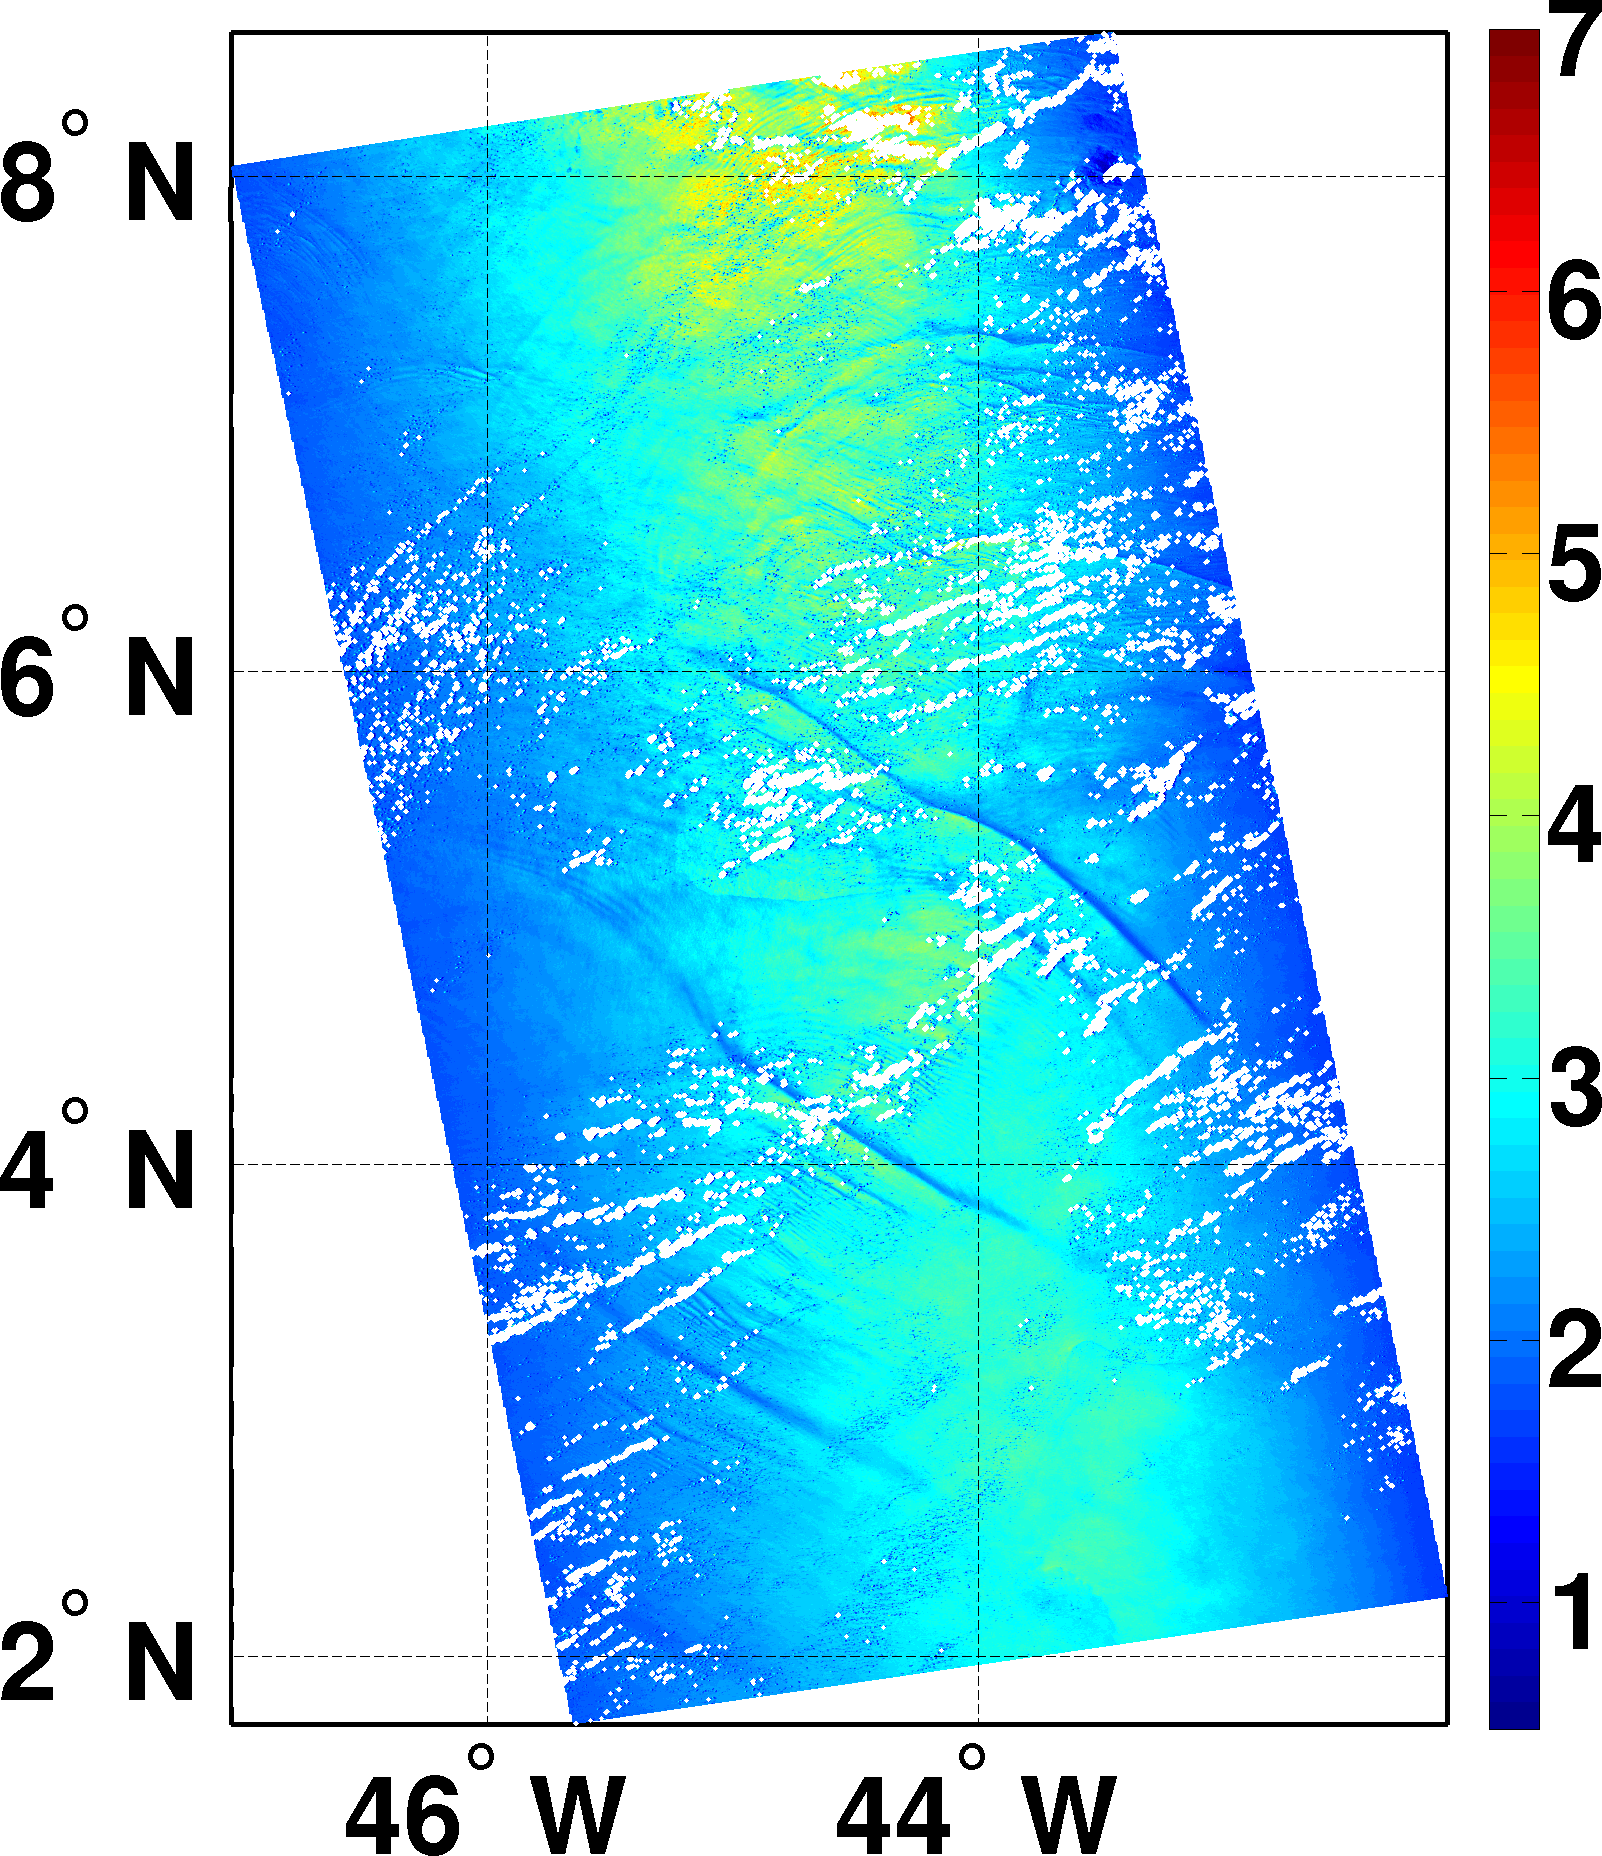
\includegraphics[width=1\linewidth]{fig3_1a}}
	\end{minipage}
	\hfill
	\begin{minipage}{.47\textwidth}
	    \subcaptionbox{\label{fig:3.1b}}
		{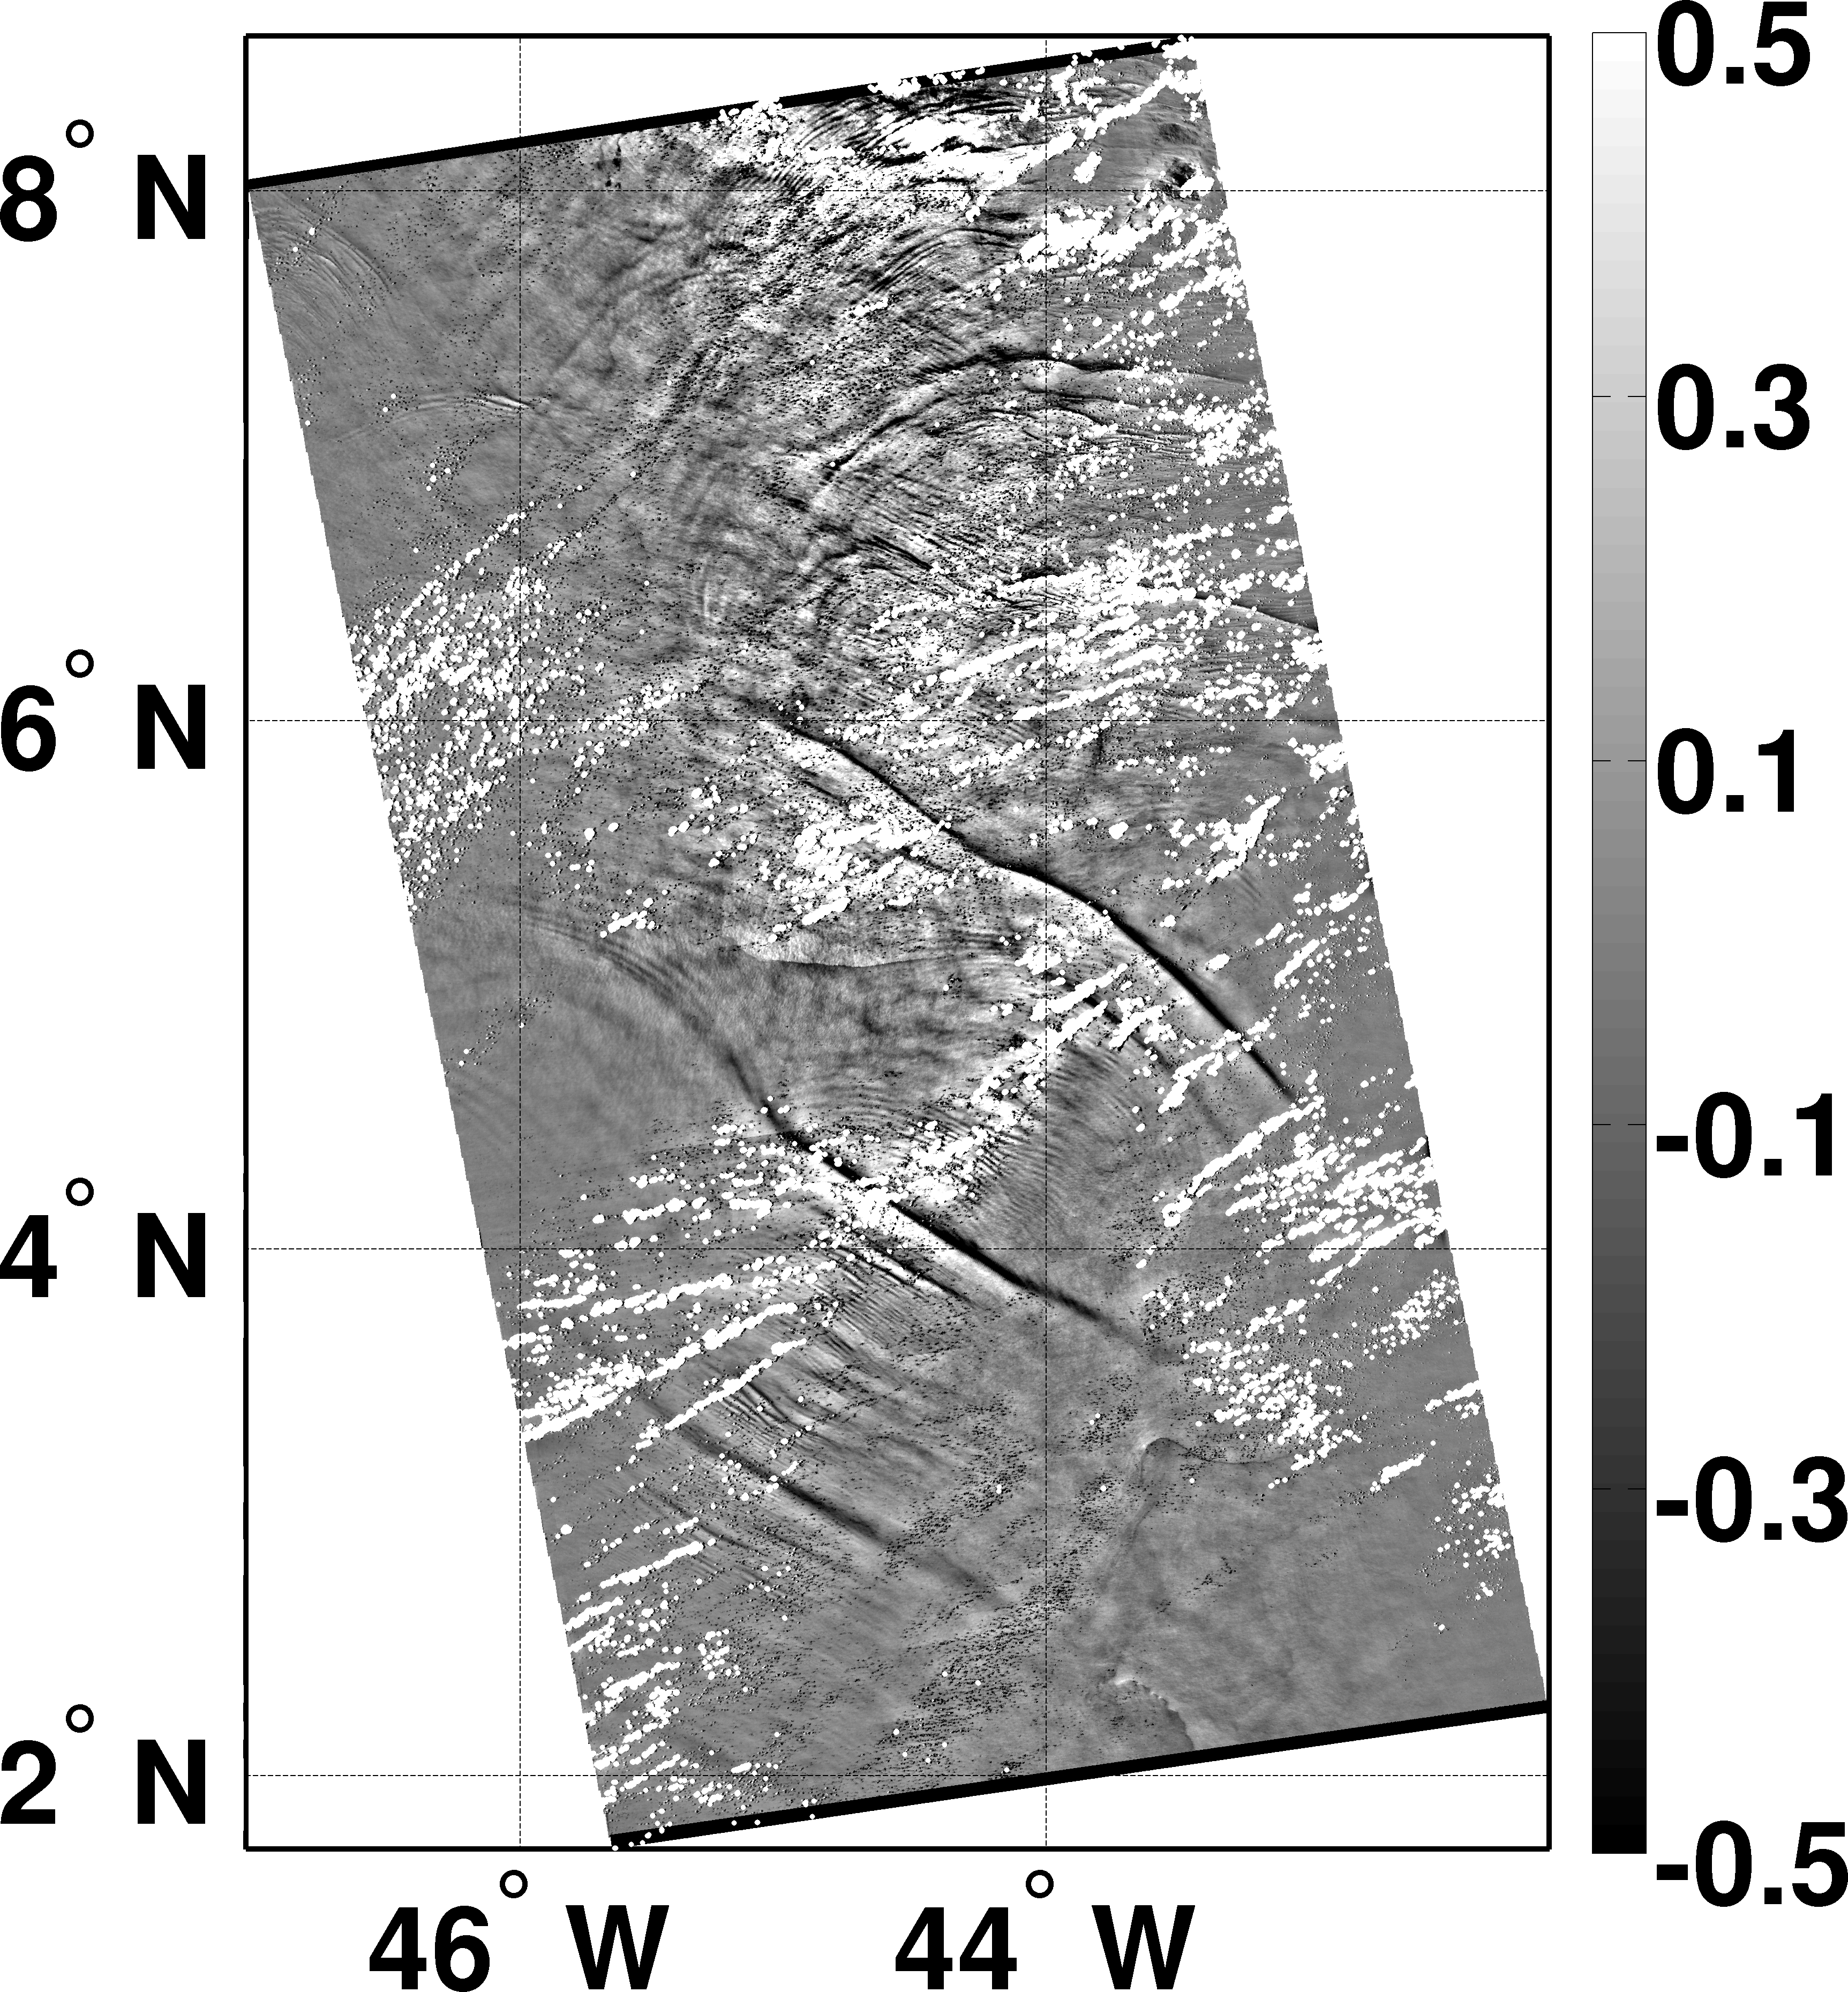
\includegraphics[width=1\linewidth]{fig3_1b}}
	\end{minipage}
	\\
	\begin{minipage}{.47\textwidth}
	    \subcaptionbox{\label{fig:3.1c}}
		{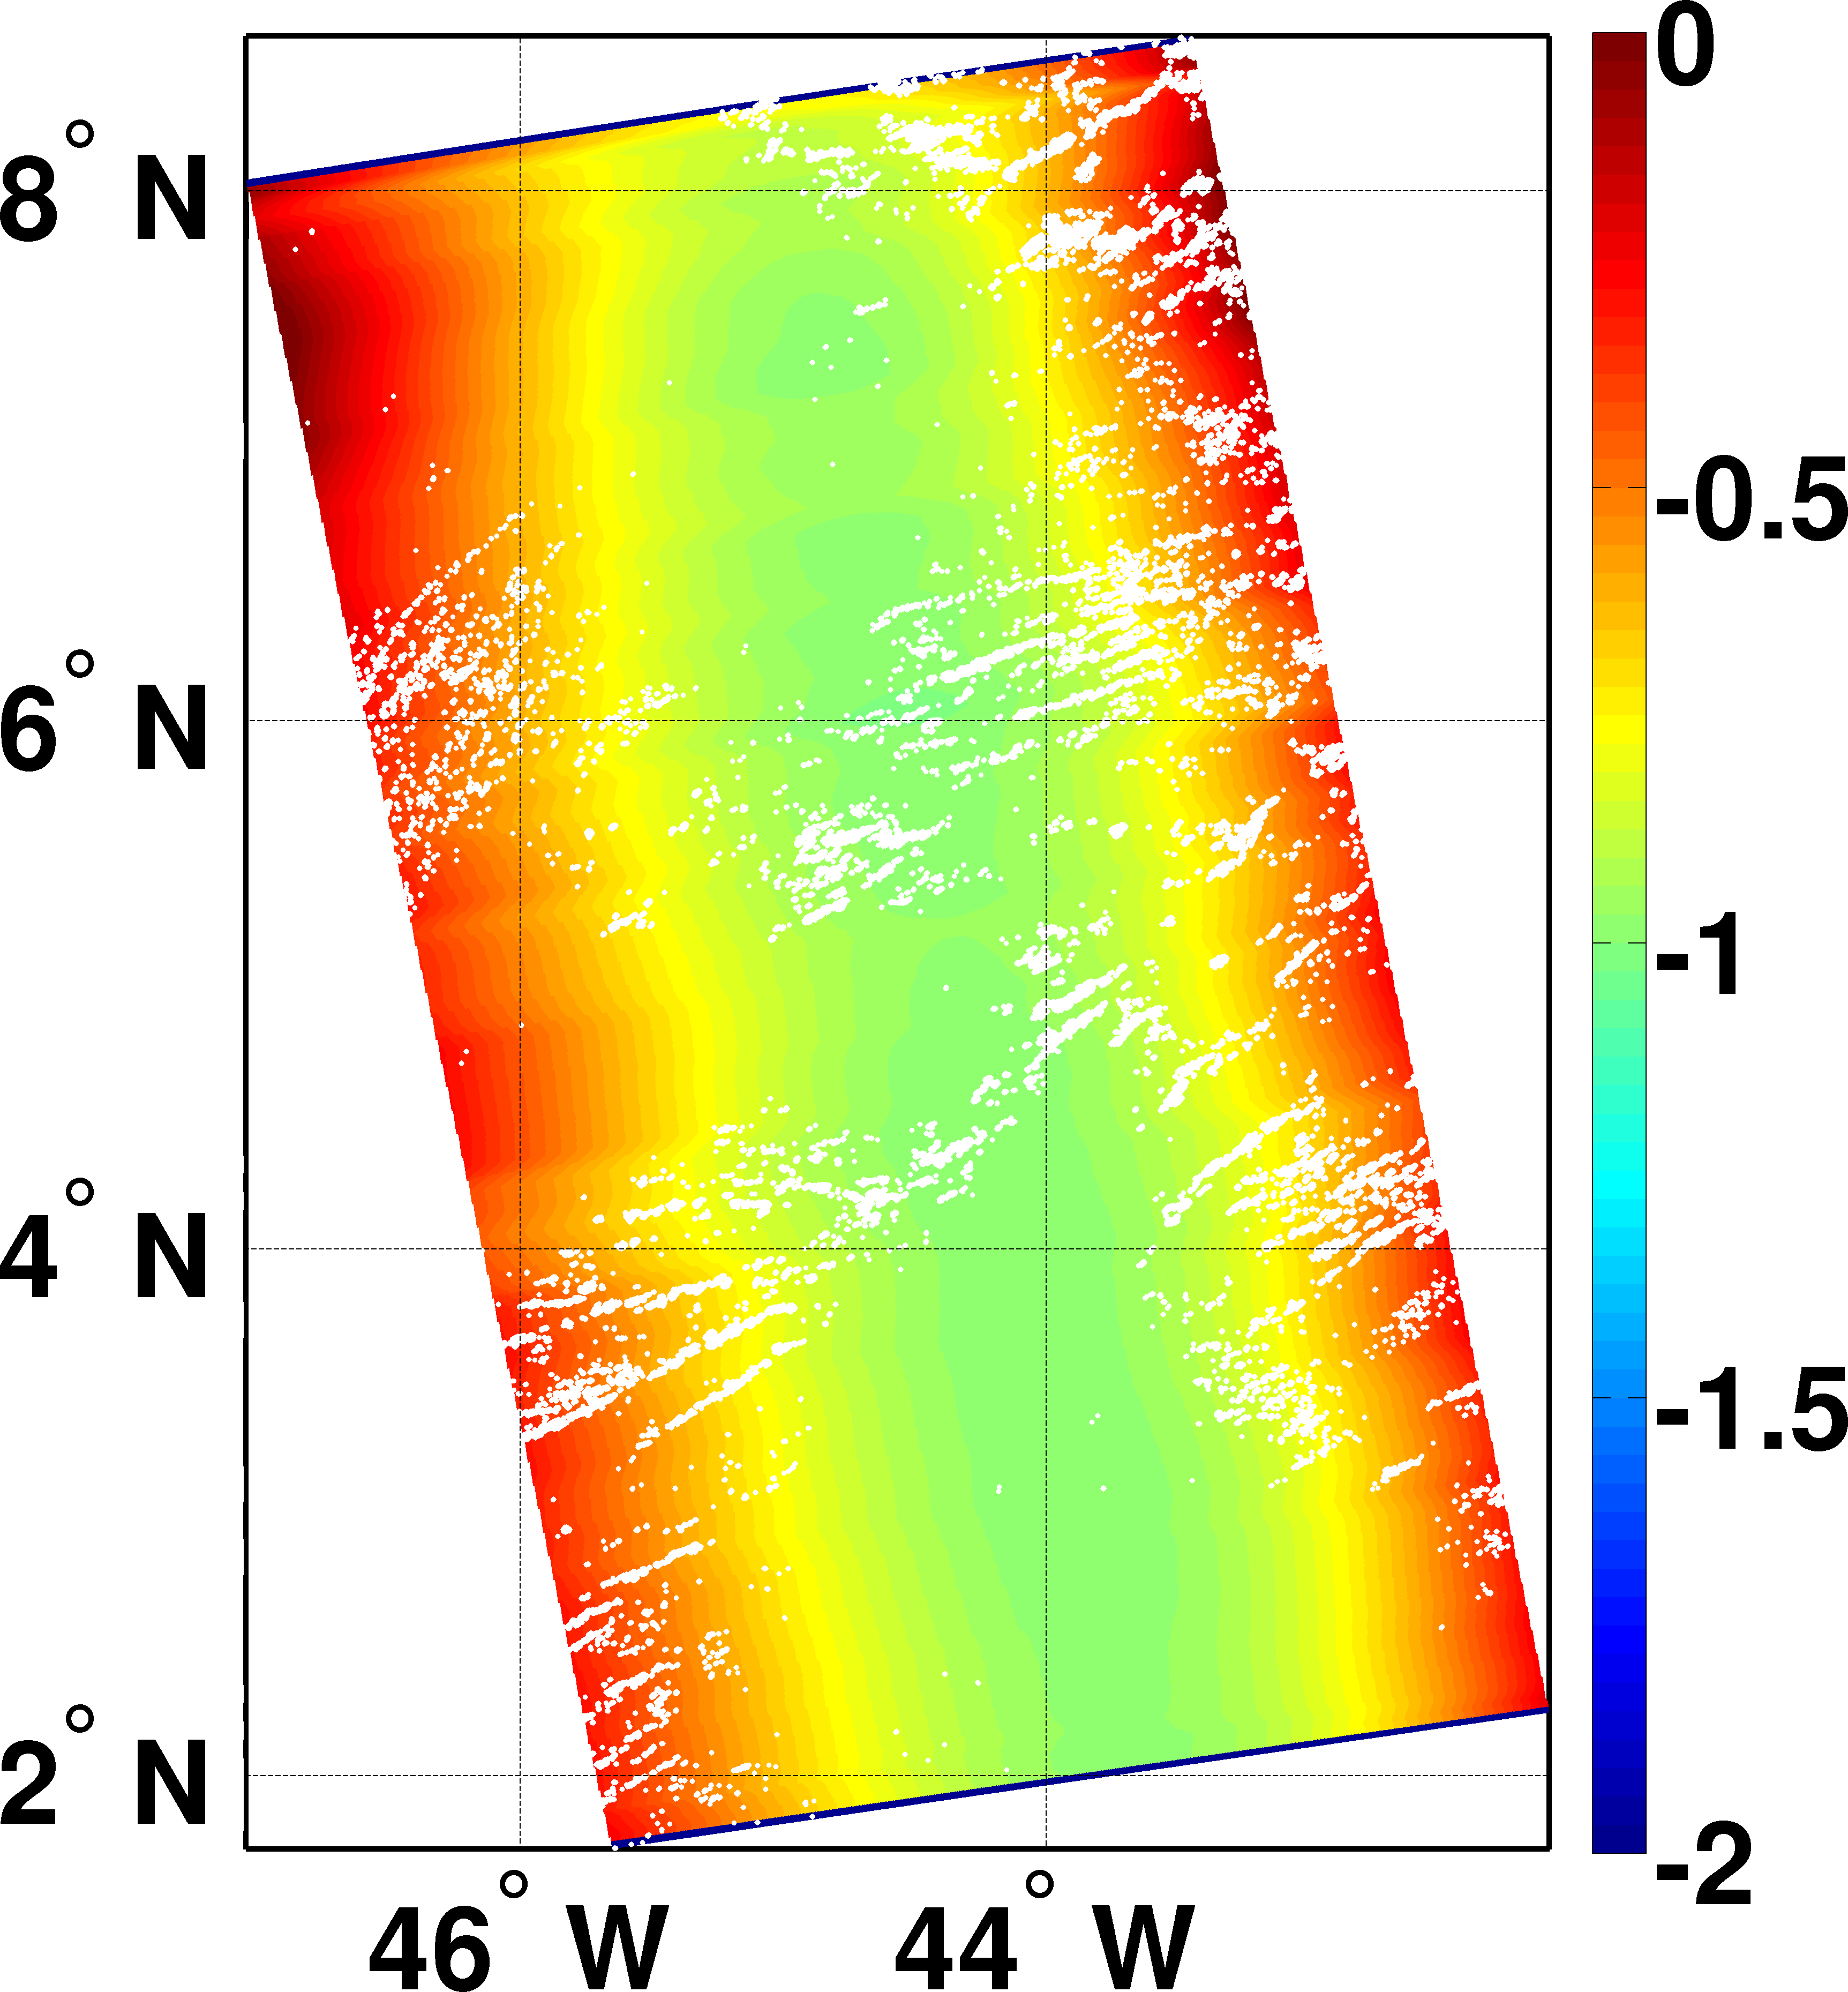
\includegraphics[width=1\linewidth]{fig3_1c}}
	\end{minipage}
	\hfill
	\begin{minipage}{.47\textwidth}
	    \subcaptionbox{\label{fig:3.1d}}
		{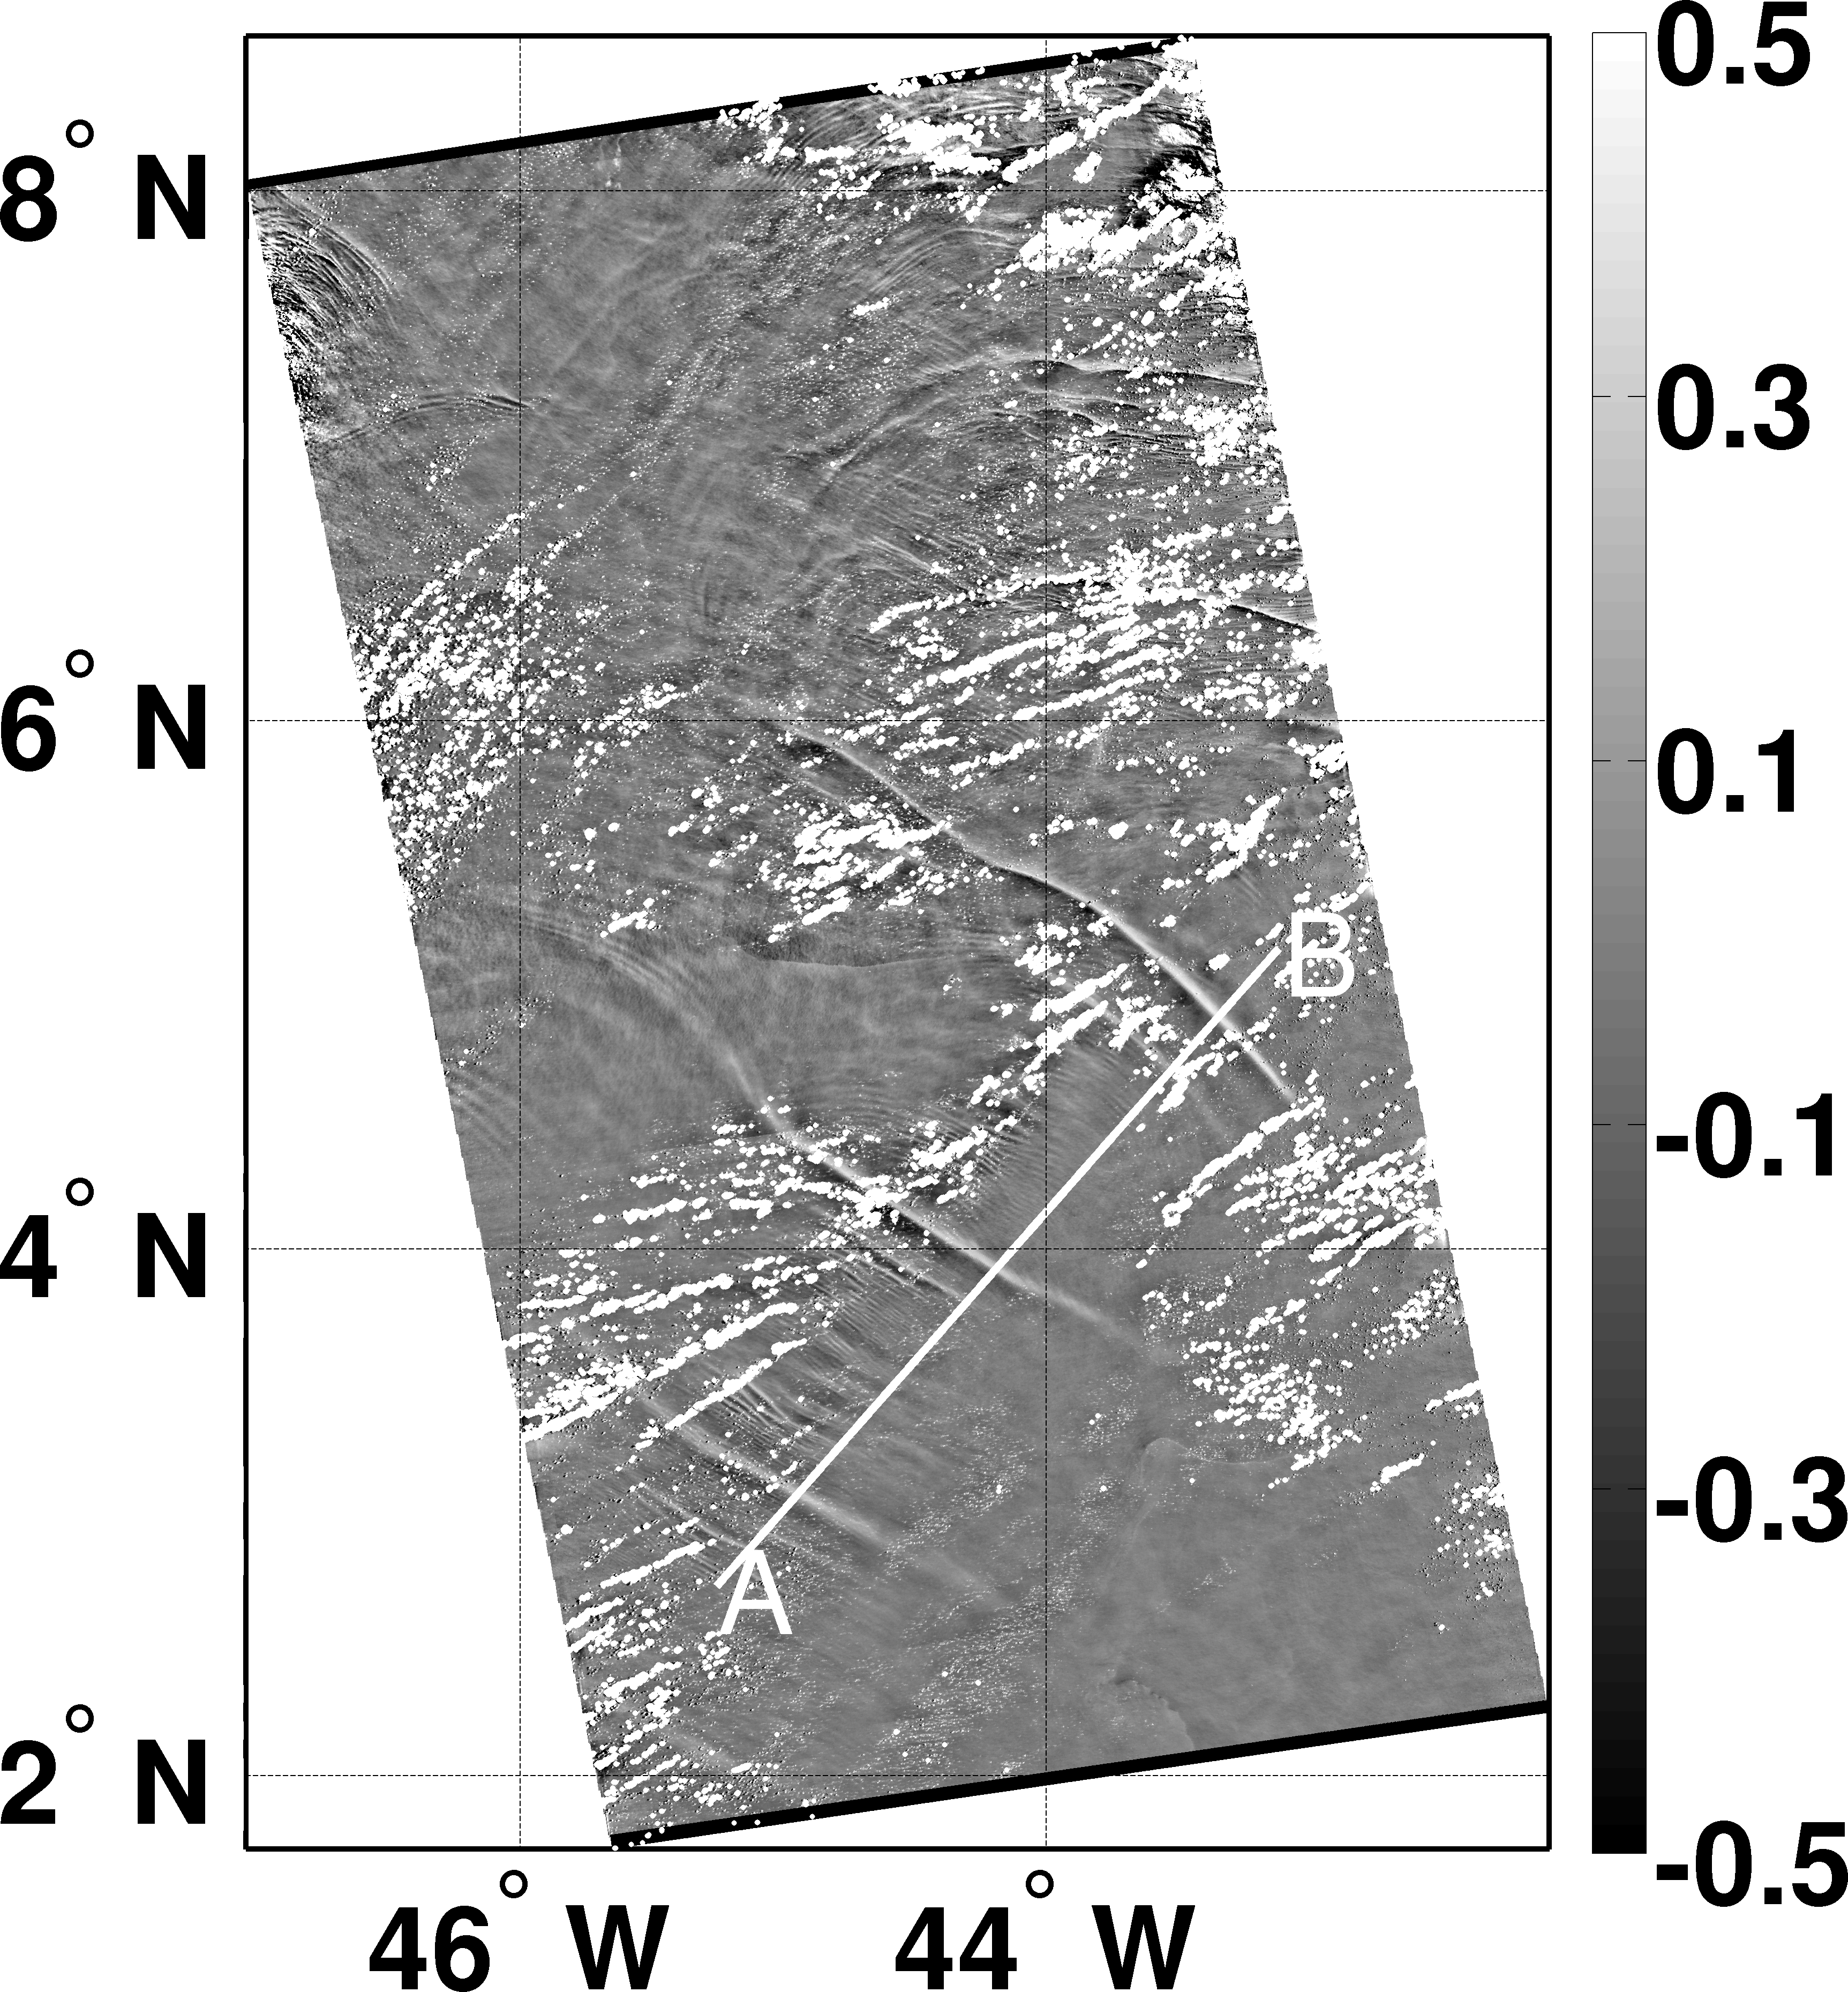
\includegraphics[width=1\linewidth]{fig3_1d}}
	\end{minipage}
    \\
    \floattitle{(а) Фрагмент исходного изображения MODIS/Aqua (26 апреля 2009, 16:20) в красном канале (645~нм) района устья реки Амазонки с признаками ВВ. (б) Контрасты яркости $\widetilde{B}/\overline{B}$. (в) Передаточная функция $T$, заданная уравнениями \eqref{eq:1.7}, \eqref{eq:1.8} и \eqref{eq:1.9}. (г) Контрасты СКН ${\widetilde{s^{2} }\mathord{\left/ {\vphantom {\widetilde{s^{2} } s^{2} }} \right. \kern-\nulldelimiterspace} s^{2} } $. Белые области на изображениях -- маска облаков. Линия A-B обозначает положение сечения, показанного на Рисунке~\ref{fig:3.2}}
    \caption{Фрагмент исходного изображения MODIS/Aqua, обработанный с применением подхода, предложенного в Главе~\ref{chap:1}}
    \label{fig:3.1}
\end{figure}


Профиль вариаций СКН вдоль сечения A-B (отмеченного на Рисунке~\ref{fig:3.1c}) представлен на Рисунке~\ref{fig:3.2},~вверху. Распределение солитонов ВВ в вариациях СКН имеет ``биполярную'' форму, с положительными и отрицательными аномалиями СКН. Возвращаясь к форме солитона ВВ, можно заключить, что повышение/уменьшение СКН имеет место в зонах конвергенции/дивергенции поверхностных течений, вызванных ВВ. Поведение контрастов СКН очень схоже с пространственными вариациями обрушений ветровых волн вызванных ВВ, которые были проанализированы в работе \citep{1986}.



\begin{figure}[H]
    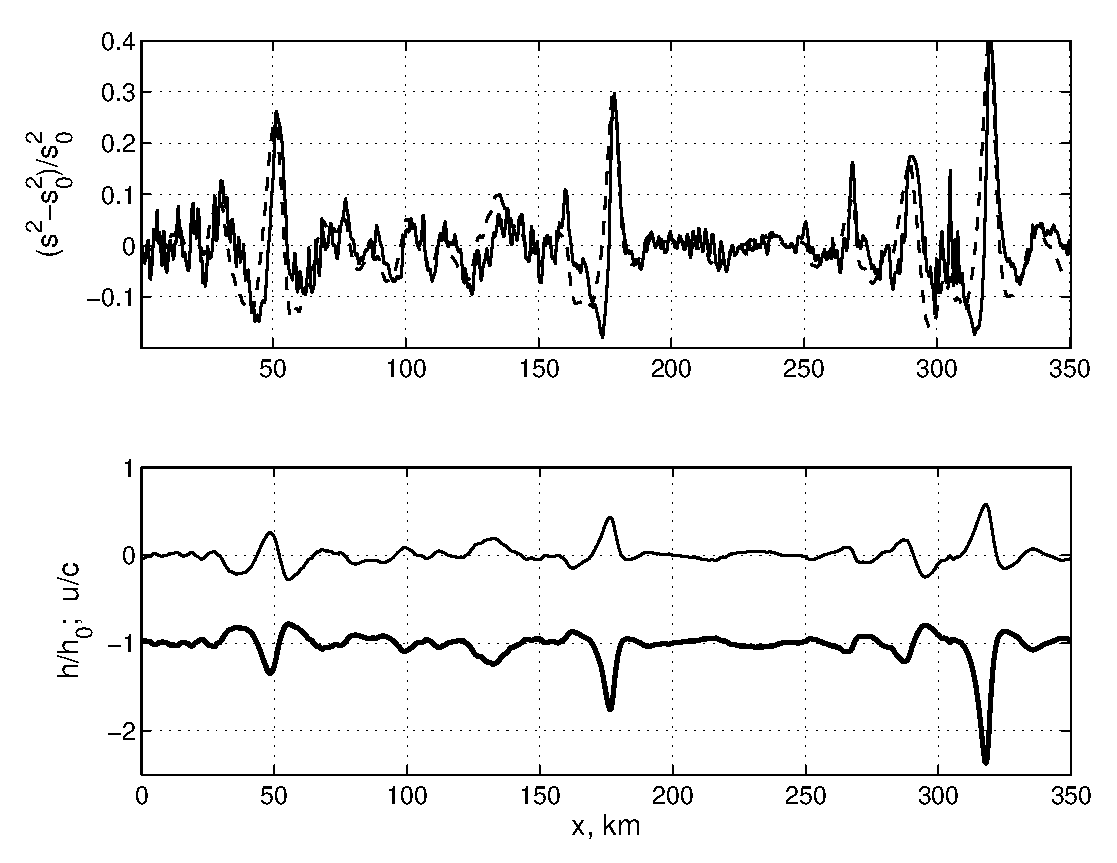
\includegraphics[width=\linewidth]{fig3_2}
    \floattitle{(вверху) Профиль контрастов СКН (сплошная линия) вдоль сечения A-B, показанного на Рисунке~\ref{fig:3.1c}. Пунктирная линия отражает RIM моделирование. (внизу) Смещение термоклина ВВ-ой (жирная линия) и скорость течения на поверхности, вызванное ВВ (тонкая линия)}
    \caption{Профиль контрастов СКН и RIM моделирование сечения, проходящего через ВВ на Рисунке~\ref{fig:3.1c}}
    \label{fig:3.2}
\end{figure}


Для анализа наблюдаемых вариаций СКН нами были проведены модельные расчёты с использованием модели формирования радиолокационных изображений (RIM), предложенной в работе \citep{Kudryavtsev2005}. (см. Приложение~\ref{AppendixA} с описанием модели) В качестве первого предположения можно положить, что наблюдаемое увеличение/уменьшение СКН морской поверхности однозначно связано с конвергенцией/дивергенцией поверхностных течений, вызванных ВВ, т.е. $K_{s} \equiv \tilde{s}^{2} /s_{0}^{2} \propto \partial u/\partial x$. Коэффициент пропорциональности в этом уравнении есть функция скорости ветра и параметров ВВ. Для заданных условий, его можно задать подгоночной константой $c_{u} $, которая определяется сравнением наблюдаемым и модельным СКН. Тогда, поверхностная скорость определяется как



\begin{equation} \label{eq:3.1} u(x)=c_{u} \int _{0}^{x}\left(K_{s} -\left\langle K_{s} \right\rangle \right)dx ,  \end{equation} 



\noindent где $\left\langle K_{s} \right\rangle $ - ``низкочастотные'' колебания СКН (вызванные, например, вариациями скорости ветра), которые не видны на представленных данных, но, приводящие к ``искусственному'' вкладу в $u(x)$, благодаря кумулятивному интегрированию. Эти ``низкочастотные'' осцилляции были вычтены из исходных данных СКН.

Далее, поверхностная скорость течений, определенная соотношением \eqref{eq:3.1}, задавалась в качестве входного параметра для модельных расчетов поверхностных проявлений ВВ по модели RIM. В этих расчетах средняя скорость ветра принята равной 7\textit{м/с}, направление ветра -- противоположным направлению распространения ВВ, а фазовая скорость ВВ задана как c=3.5\textit{м/с}. Значение постоянной $c_{u} $ выбиралась таким образом, чтобы значения вариаций СКН в пиках (над солитонами ВВ) соответствовало бы наблюдаемым значениям. Модельные контрасты СКН показаны на Рисунке~\ref{fig:3.2},~верхний график. Как следует из этого рисунка (Рисунок~\ref{fig:3.2}), профиль модельных контрастов согласуется с наблюдаемым полем вариаций СКН. Это факт позволяет заключить, что наблюдаемые модуляции СКН, в действительности, определяются конвергенцией и дивергенцией течений, индуцируемой ВВ на поверхности. образованных ВВ.

Поле поверхностной скорости $u(x)$, индуцируемое ВВ, а так же как соответствующая глубина залегания термоклина $h(x)$ (рассчитанная с использованием формулы $u/c=(h-h_{0} )/h$, где $h_{0} $ - невозмущённая глубина) приведены на Рисунке~\ref{fig:3.2},~нижний график. Полагая h0=100\textit{м}, амплитуды смещения термоклина $h-h_{0} $ для двух ведущих солитонов составляют 120\textit{м} и 80\textit{м}, что согласуется с данными измерений (Dulov et al., 1986) в этом районе.



\section{Мезомасштабные течения} \label{sec:3.2}



\subsection{Наблюдения} \label{sec:3.2.1}


Данное исследование основано на синергетике изображений MODIS и ASAR района течения мыса Игольный (Рисунок~\ref{fig:3.3}). Этот район характеризуется интенсивным течением, которое обеспечивает разнообразие мезомасштабной динамики (вихри, грибовидные структуры, температурные фронты, внутренние волны, зыбь и многие другие явления проявления океанической динамики). Основные продукты данных MODIS -- параметры цвета океана и температура морской поверхности. Данные ASAR могут быть эффективно использованы при изучении полей ветра, нефтяных разливов и направления течений.

Данные ASAR и MODIS/Aqua в районе исследования были получены 18 ноября 2007~г. В 7 ч.~24 мин. и 12 ч.~05 мин., соответственно. На Рисунке~\ref{fig:3.3} приводятся два основных продукта ASAR и MODIS -- поле ветра, полученное по изображению ASAR WS, с использованием алгоритма CMOD4, и поле ТПО, полученное по данным MODIS \citep{Brown1999}.

Поле ТПО раскрывает разнообразие мезо- и крупномасштабных особенностей на поверхности основного течения мыса Игольный. Подобные особенности можно наблюдать и в поле концентрации хлорофилла, полученного по данным MODIS (не приводится здесь). Наличие сильного приводного ветра проявляет сильную атмосферную изменчивость, в данном районе скорость ветра варьируется от 4\textit{м/с} до 13\textit{м/с}. С другой стороны на данных поля ветра ASAR легко различимы квазилинейные структуры (между 34 и 36 градусом южной широты и 26 и 30 градусом восточной долготы), которые можно трактовать как особенности проявления океанического течения. Далее приводится более глубокий анализ этих данных.



\begin{figure}[H]
   	\centering
	\begin{minipage}{.47\textwidth}
	    \subcaptionbox{\label{fig:3.3a}}
		{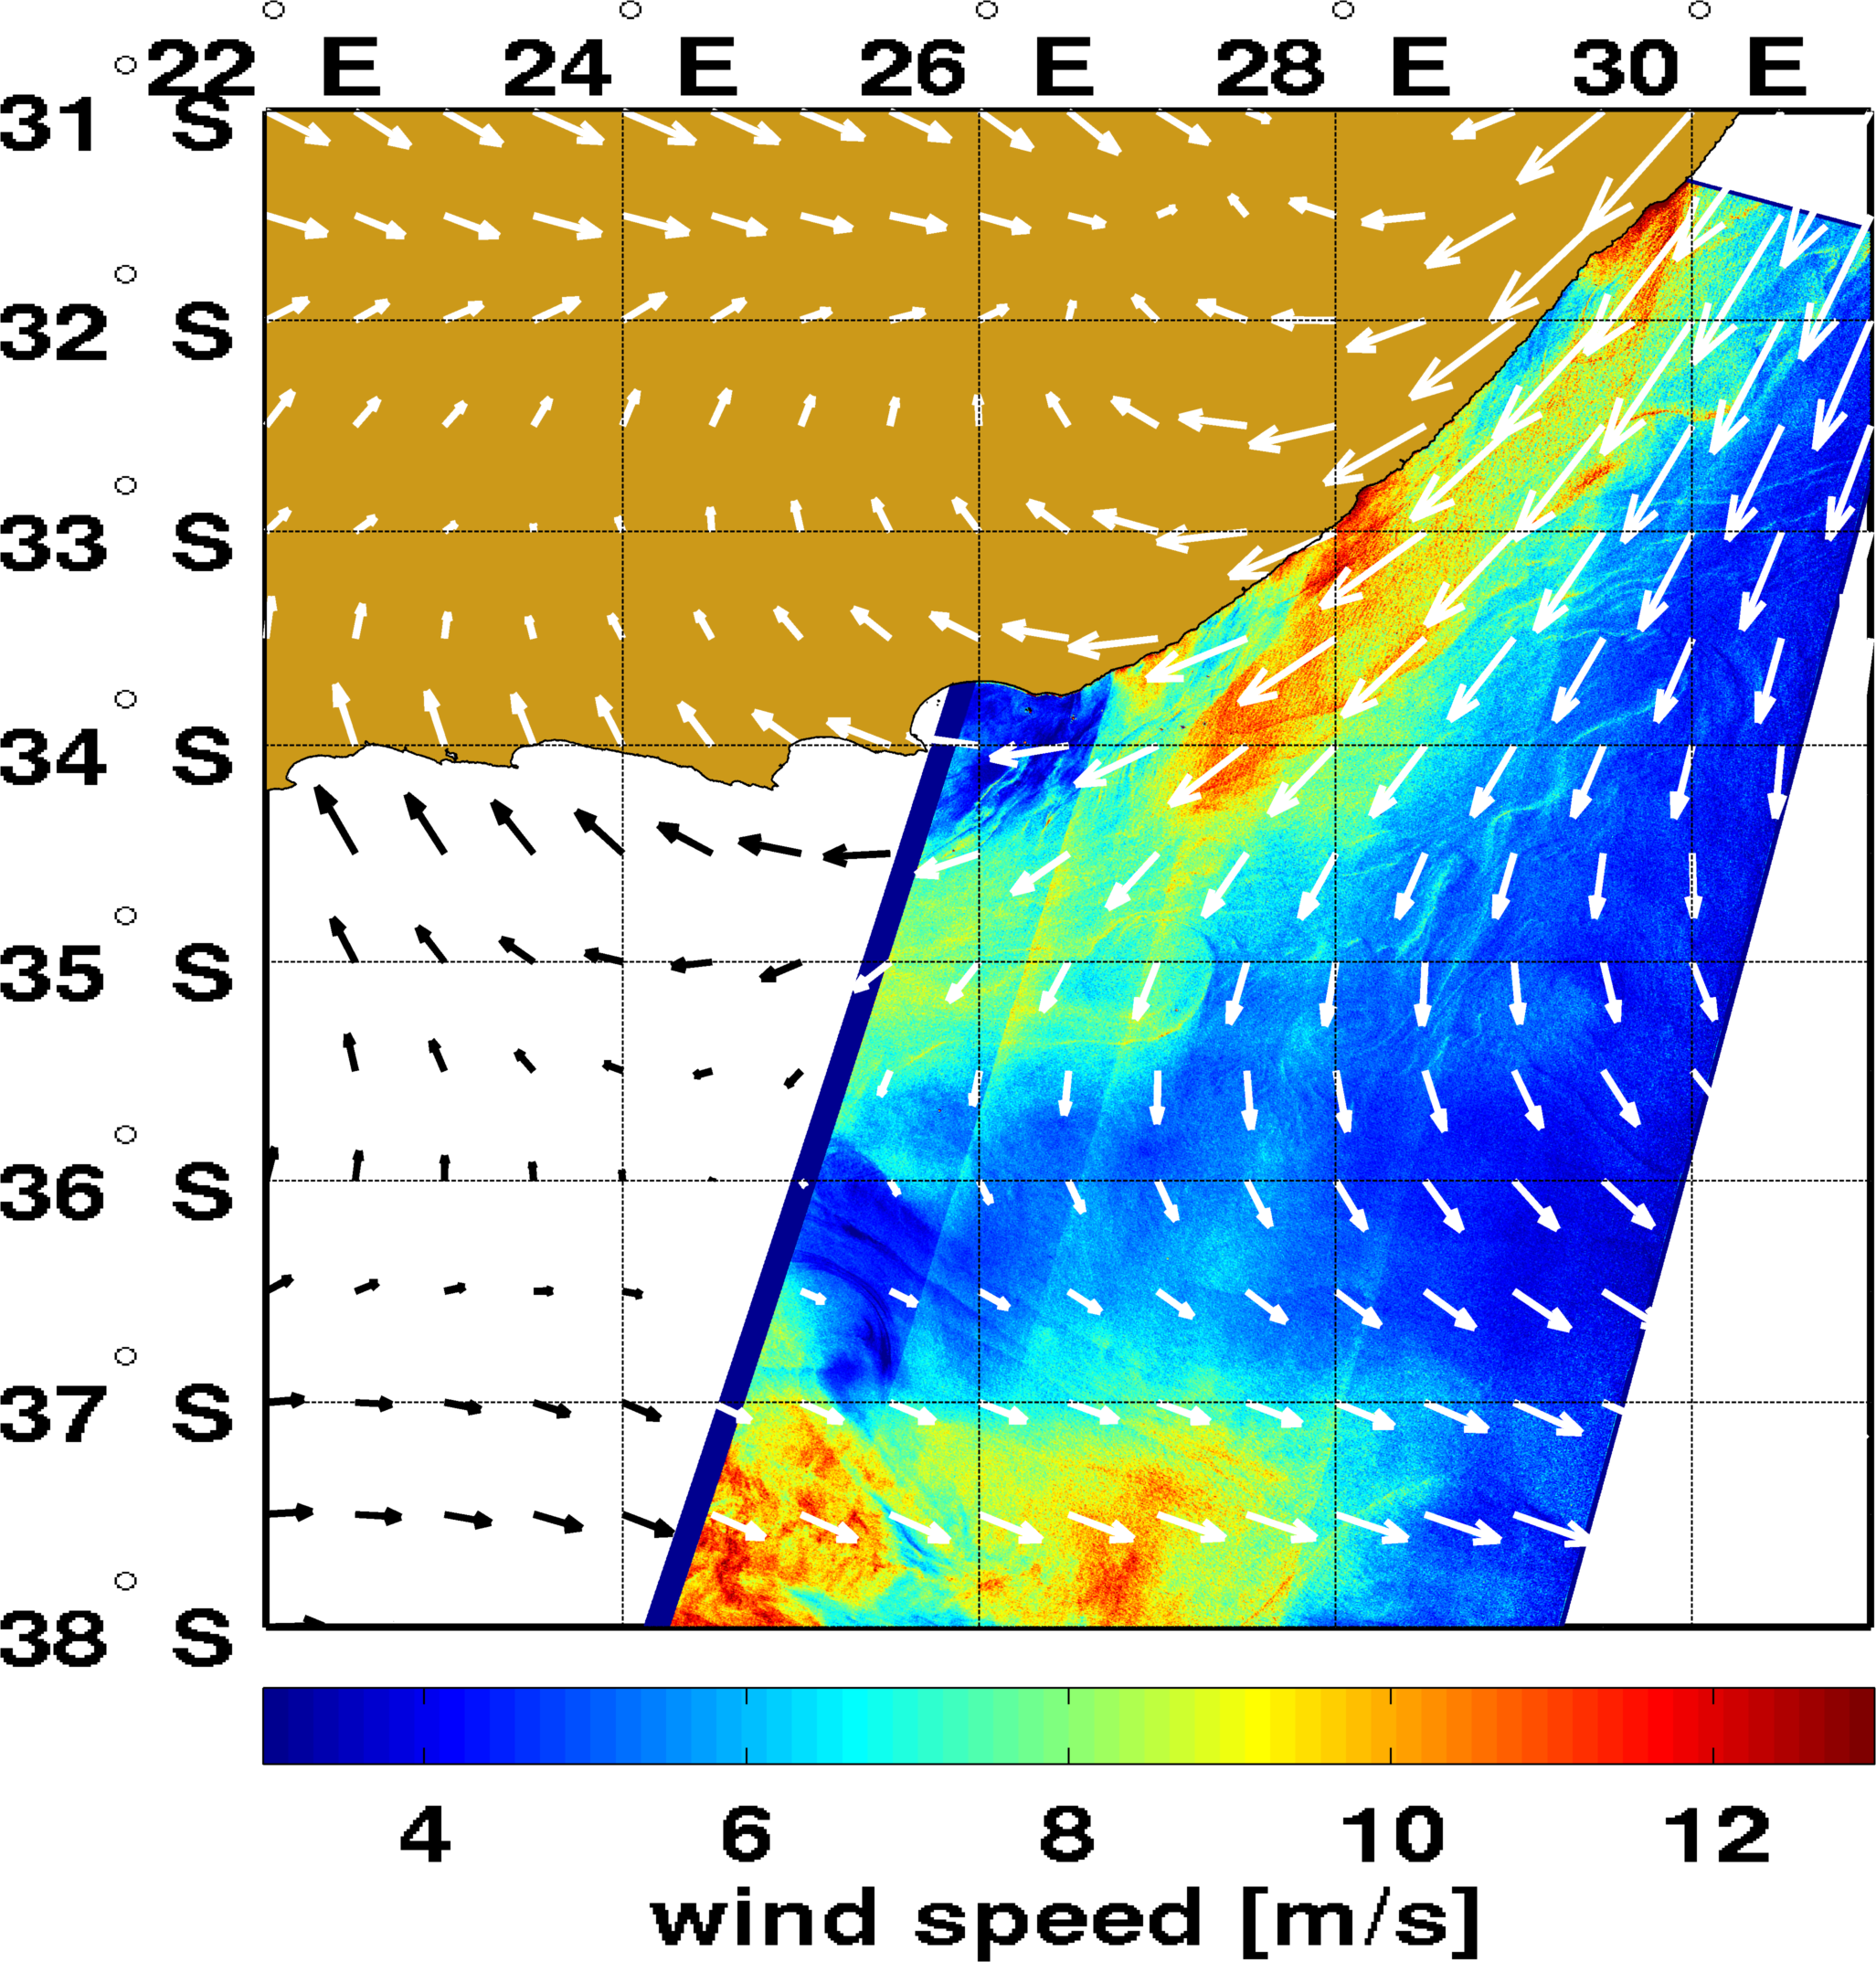
\includegraphics[width=1\linewidth]{fig3_3a}}
	\end{minipage}
	\hfill
	\begin{minipage}{.47\textwidth}
	    \subcaptionbox{\label{fig:3.3b}}
		{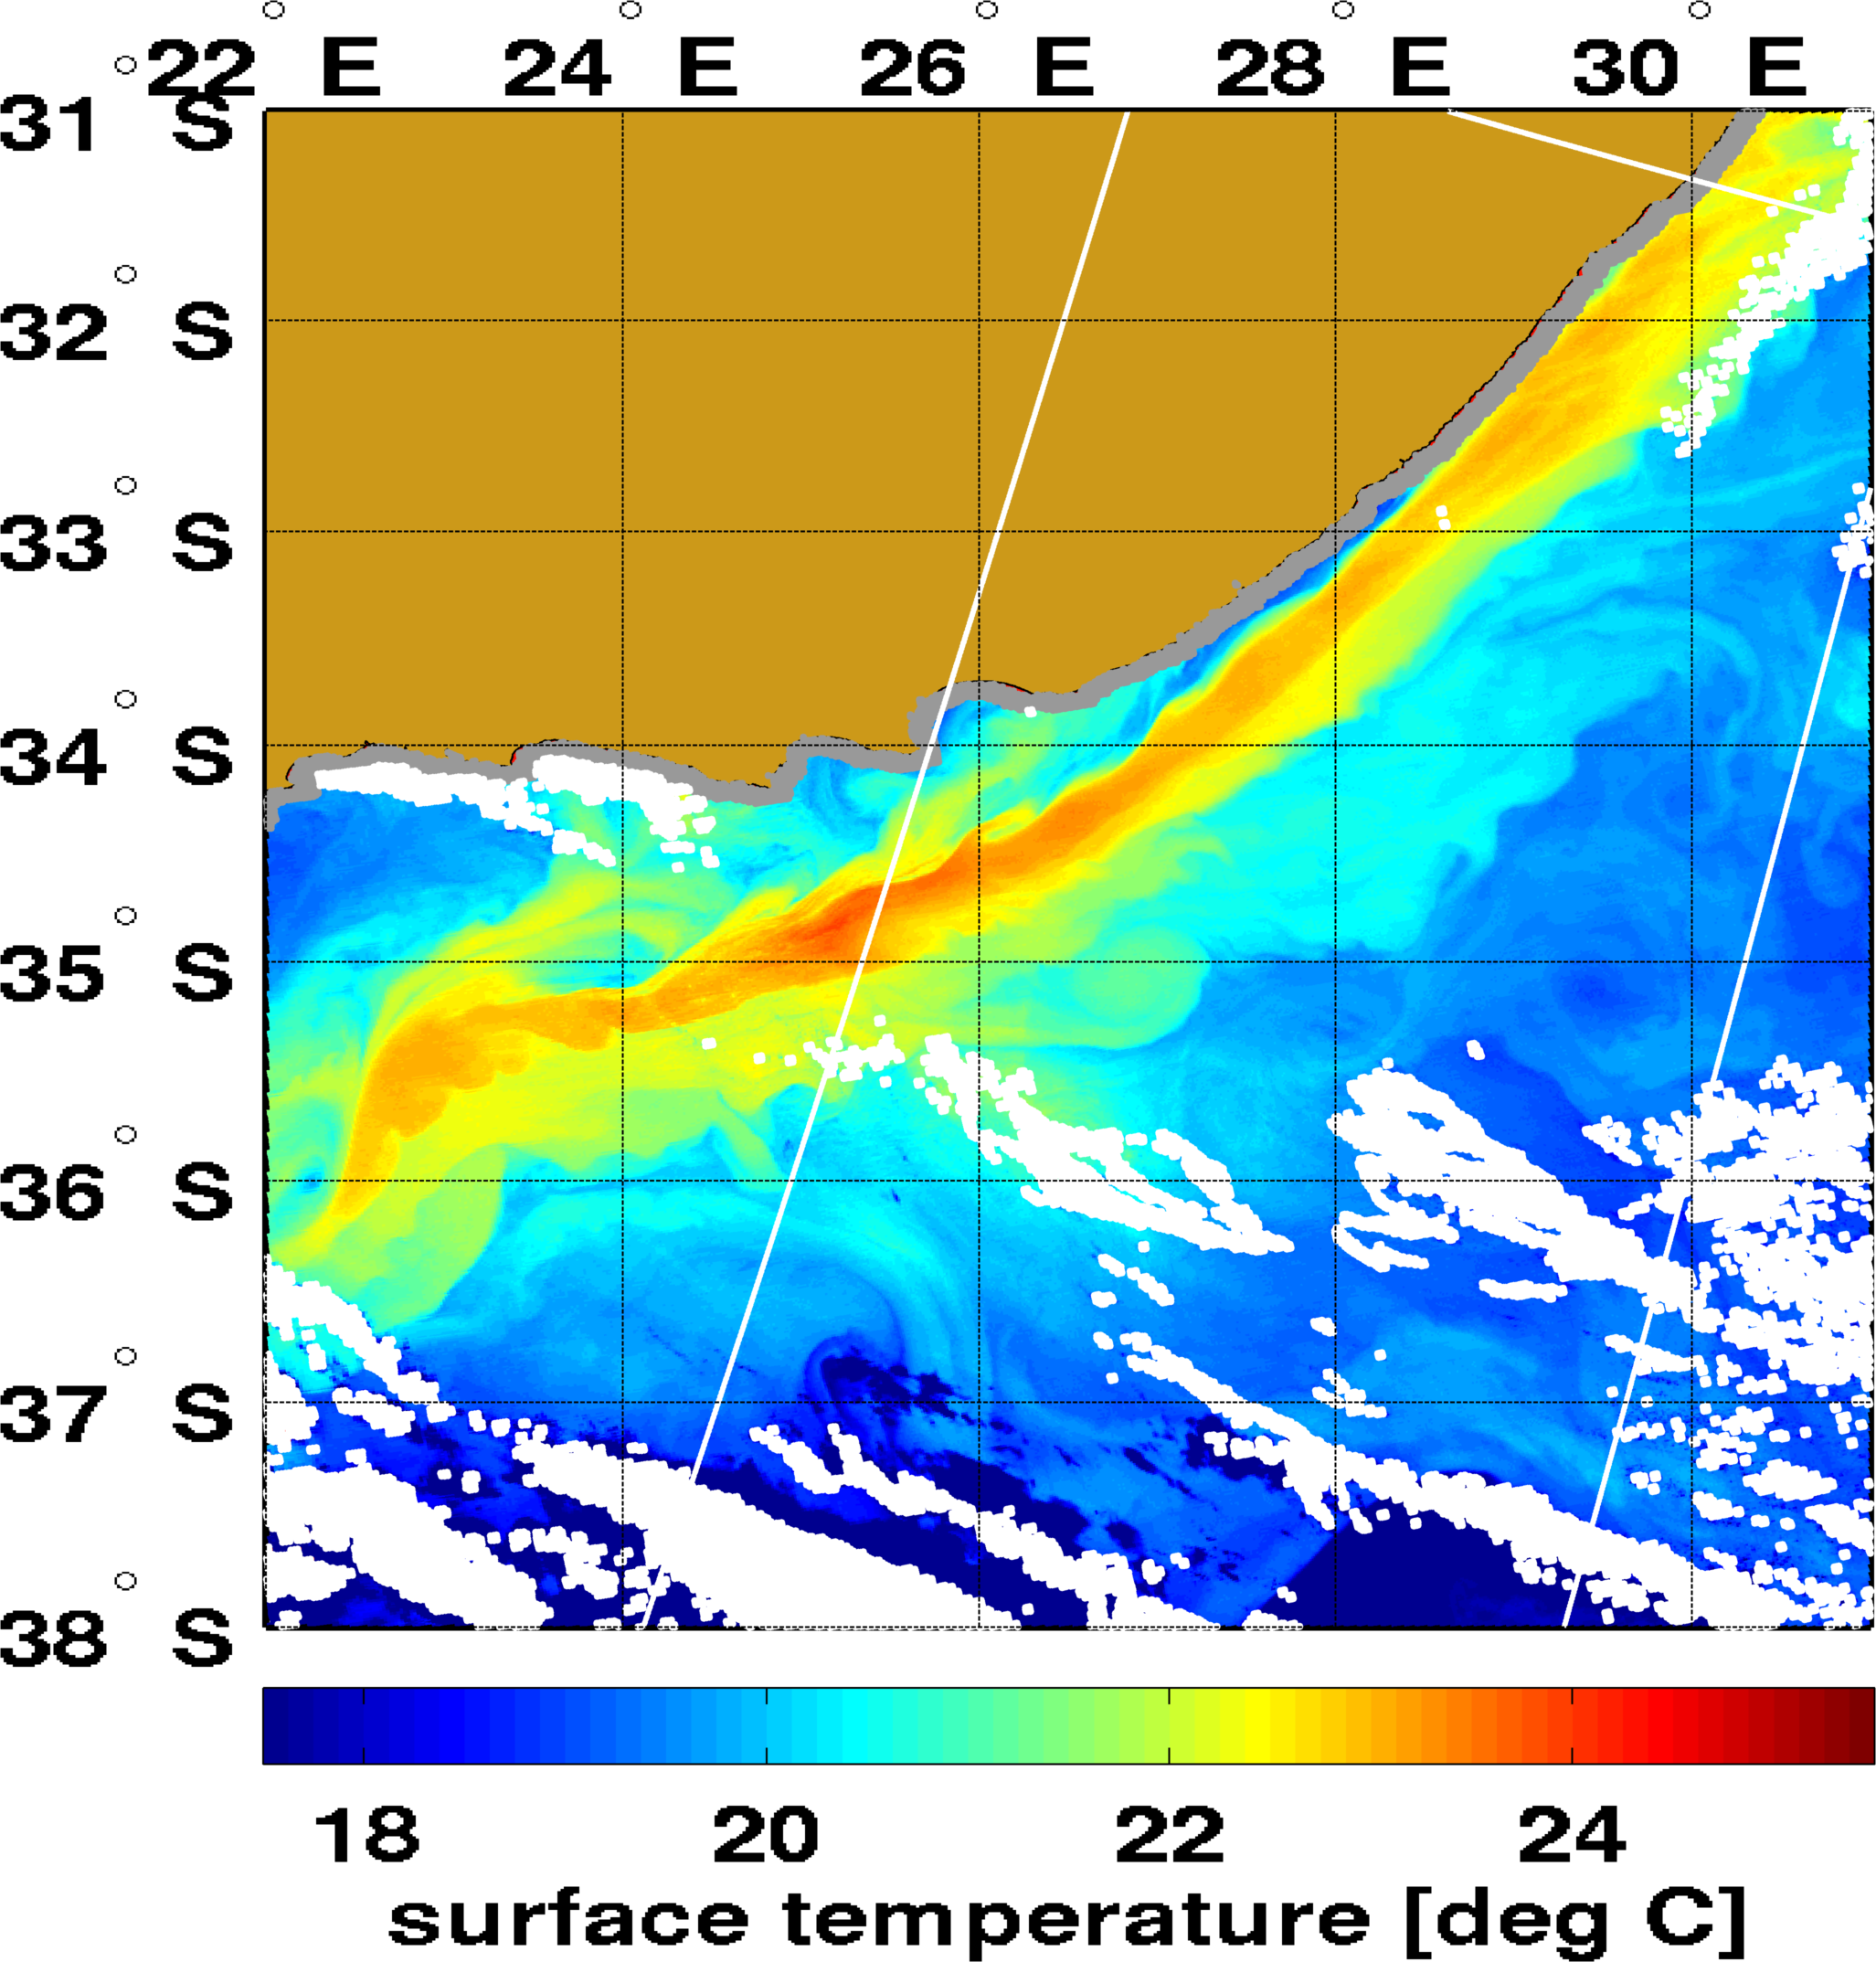
\includegraphics[width=1\linewidth]{fig3_3b}}
	\end{minipage}
    \\
    \floattitle{(а) Поле ветра, полученное по изображению ASAR WS, с использованием алгоритма CMOD4. Направление ветра взято из модели NCEP. (б) поле поверхностной температуры океана, полученное по данным MODIS. Белые области - маска облаков. Юг Африканского континента выделен коричневым цветом}
    \caption{Поле ветра и поле поверхностной температуры океана}
    \label{fig:3.3}
\end{figure}


На исходном изображении MODIS/Aqua района мыса Игольный, красный канал разрешением 250\textit{м}, приведённое на Рисунке~\ref{fig:3.4a}, легко различимы облака и солнечный блик. К интересным особенностям этого изображения стоит отнести полосчатую структуру изображения в области солнечного блика, присущую изображениям MODIS. Об особенностях формирования изображений MODIS, приводящих к подобной структуре изображения, рассказано в разделе~\ref{sec:1.4}, а также в статьях~\citep{Myasoedov2010a, Myasoedov2010}. Также стоит обратить внимание на правый край солнечного блика, где выделяется структура, похожая на океанический вихрь.

Используя алгоритм, впервые предложенный авторами в \citep{Kudryavtsev2010,Myasoedov2010a}, а также описанный в \citep{Myasoedov2010}, исходное изображение раскладывается на составляющие: усреднённые яркости $\bar{B}$ (масштаб осреднения 30x30\textit{км${}^2$}) и их вариации $\tilde{B}$. Последние приведены на Рисунке~\ref{fig:3.4b}. Здесь и далее мы опускаем детали восстановления СКН, напомним лишь, что данные MODIS и MERIS обрабатывались в соответствии с алгоритмом, описанным в разделе \ref{sec:1.3} (см. также раздел 3.2 \citep{Myasoedov2010}).



\begin{figure}[H]
   	\centering
	\begin{minipage}{.47\textwidth}
	    \subcaptionbox{\label{fig:3.4a}}
		{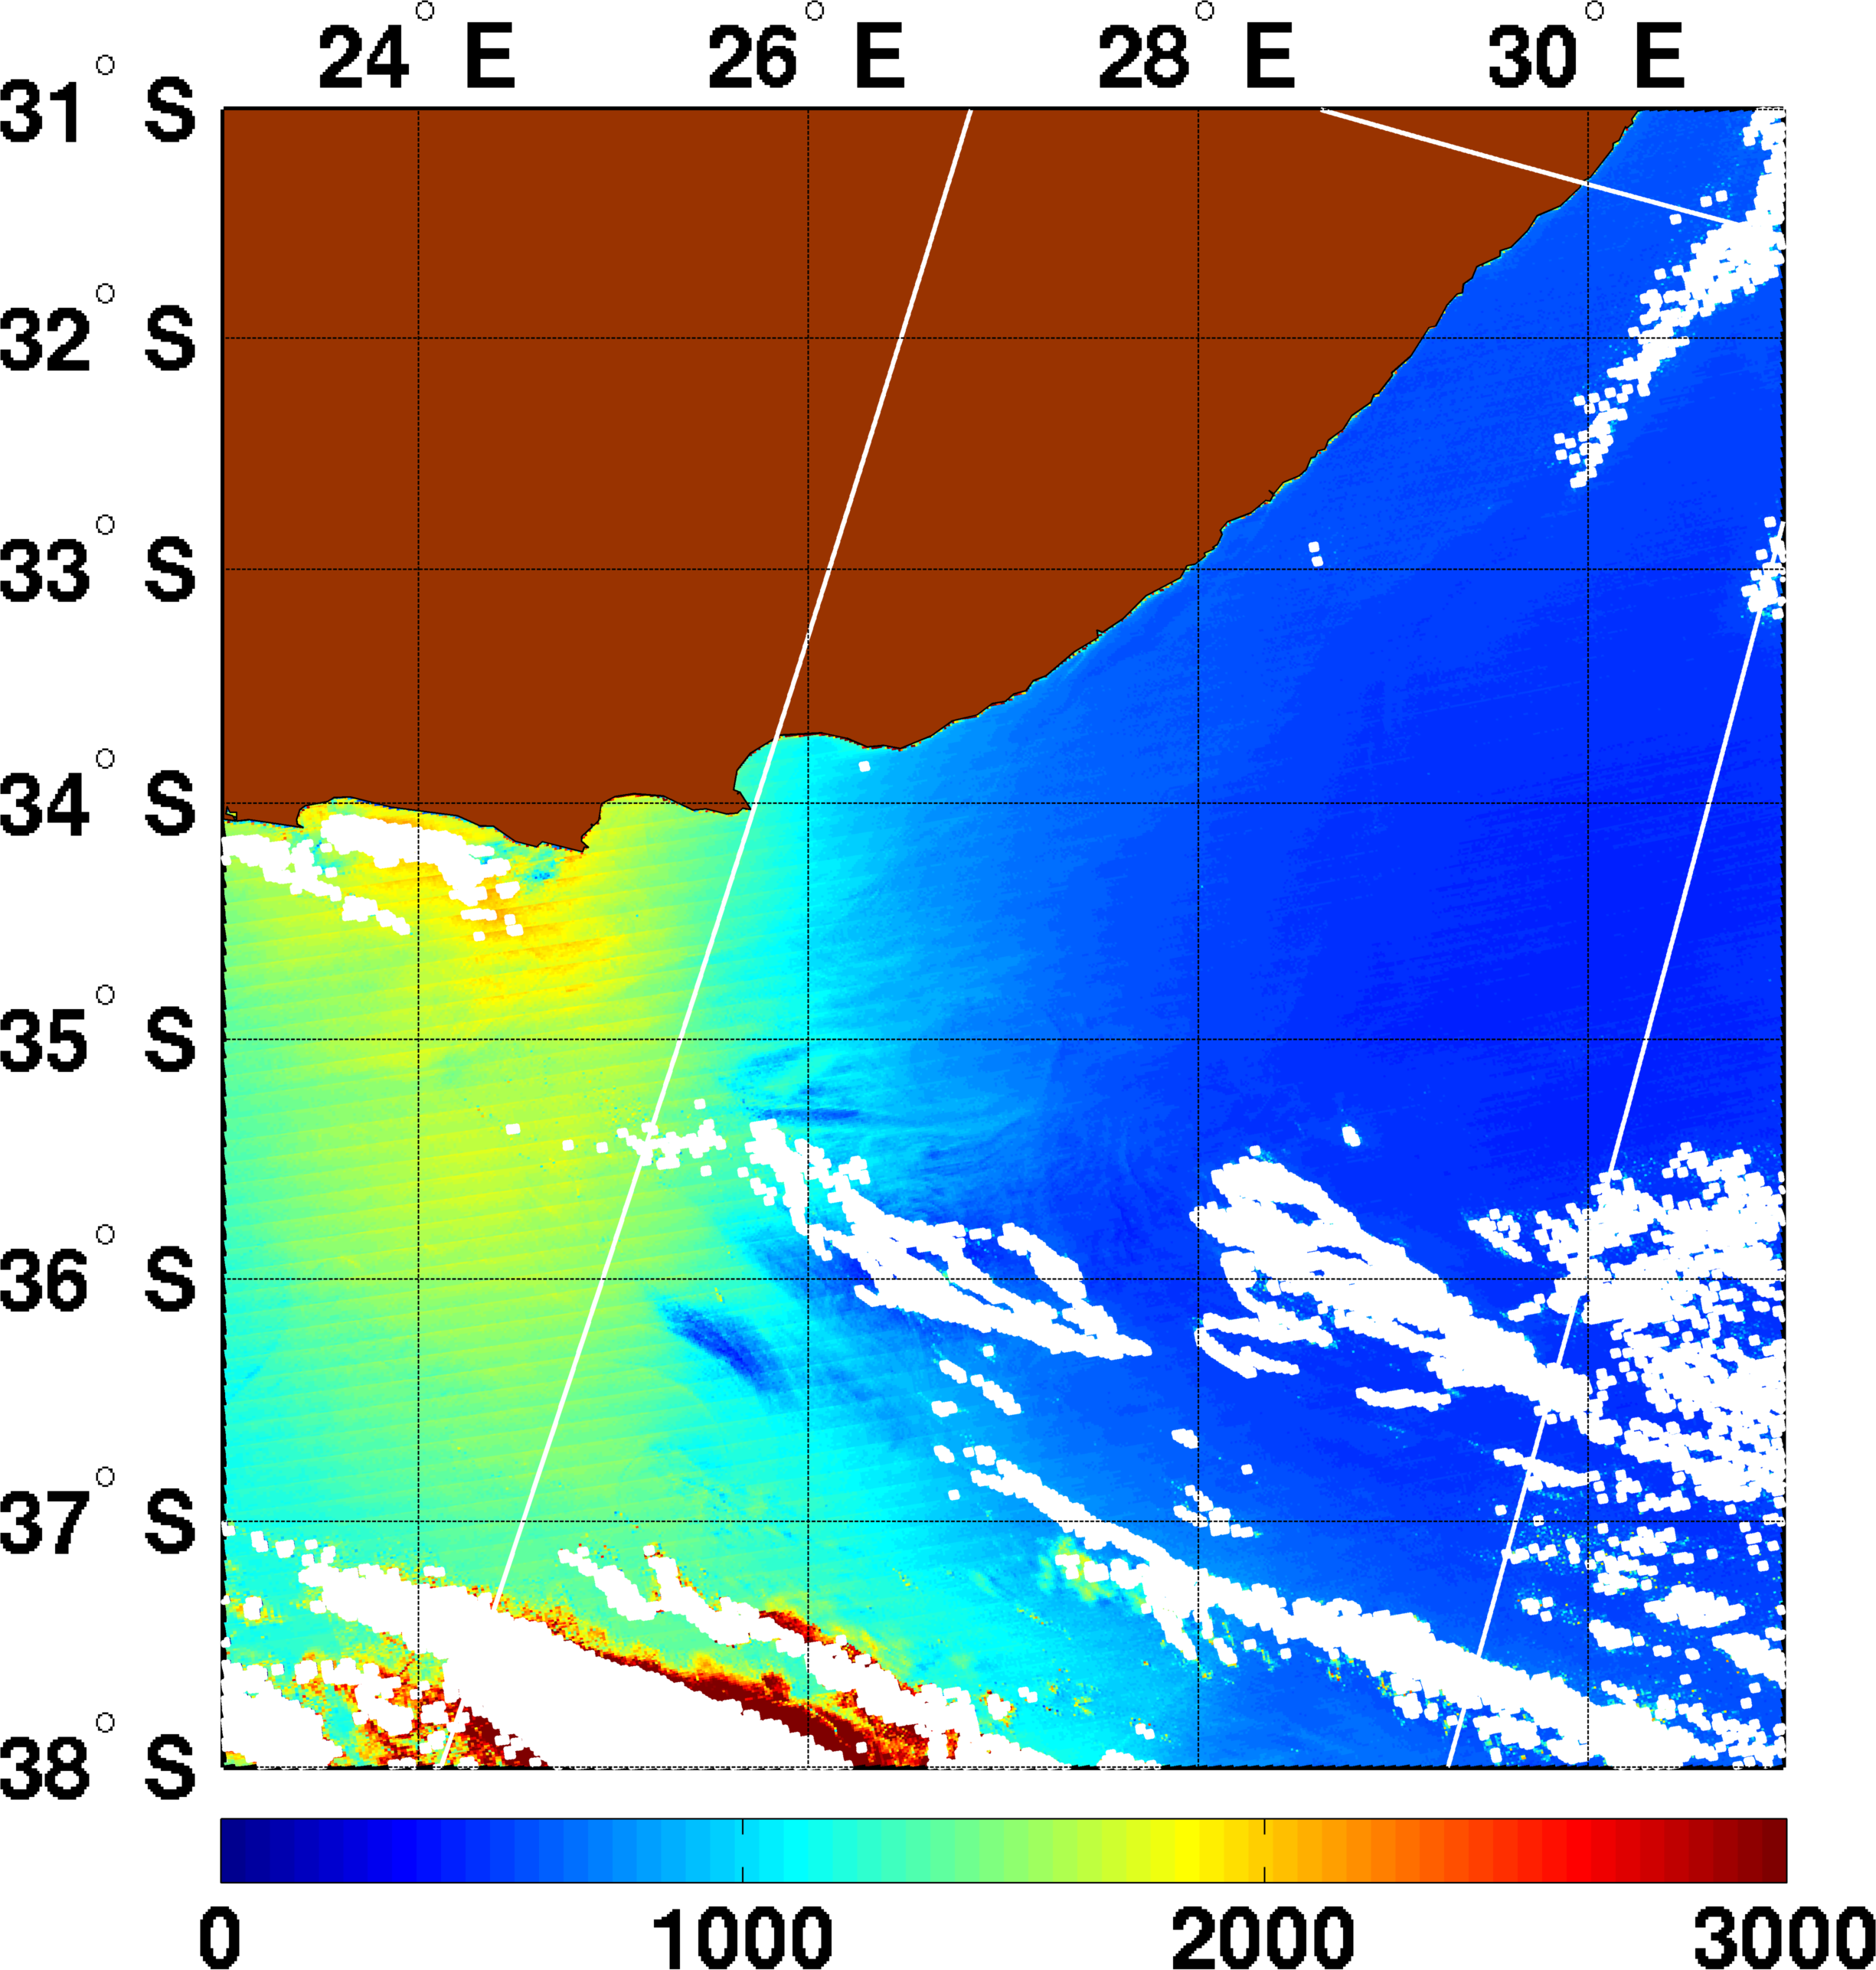
\includegraphics[width=1\linewidth]{fig3_4a}}
	\end{minipage}
	\hfill
	\begin{minipage}{.47\textwidth}
	    \subcaptionbox{\label{fig:3.4b}}
		{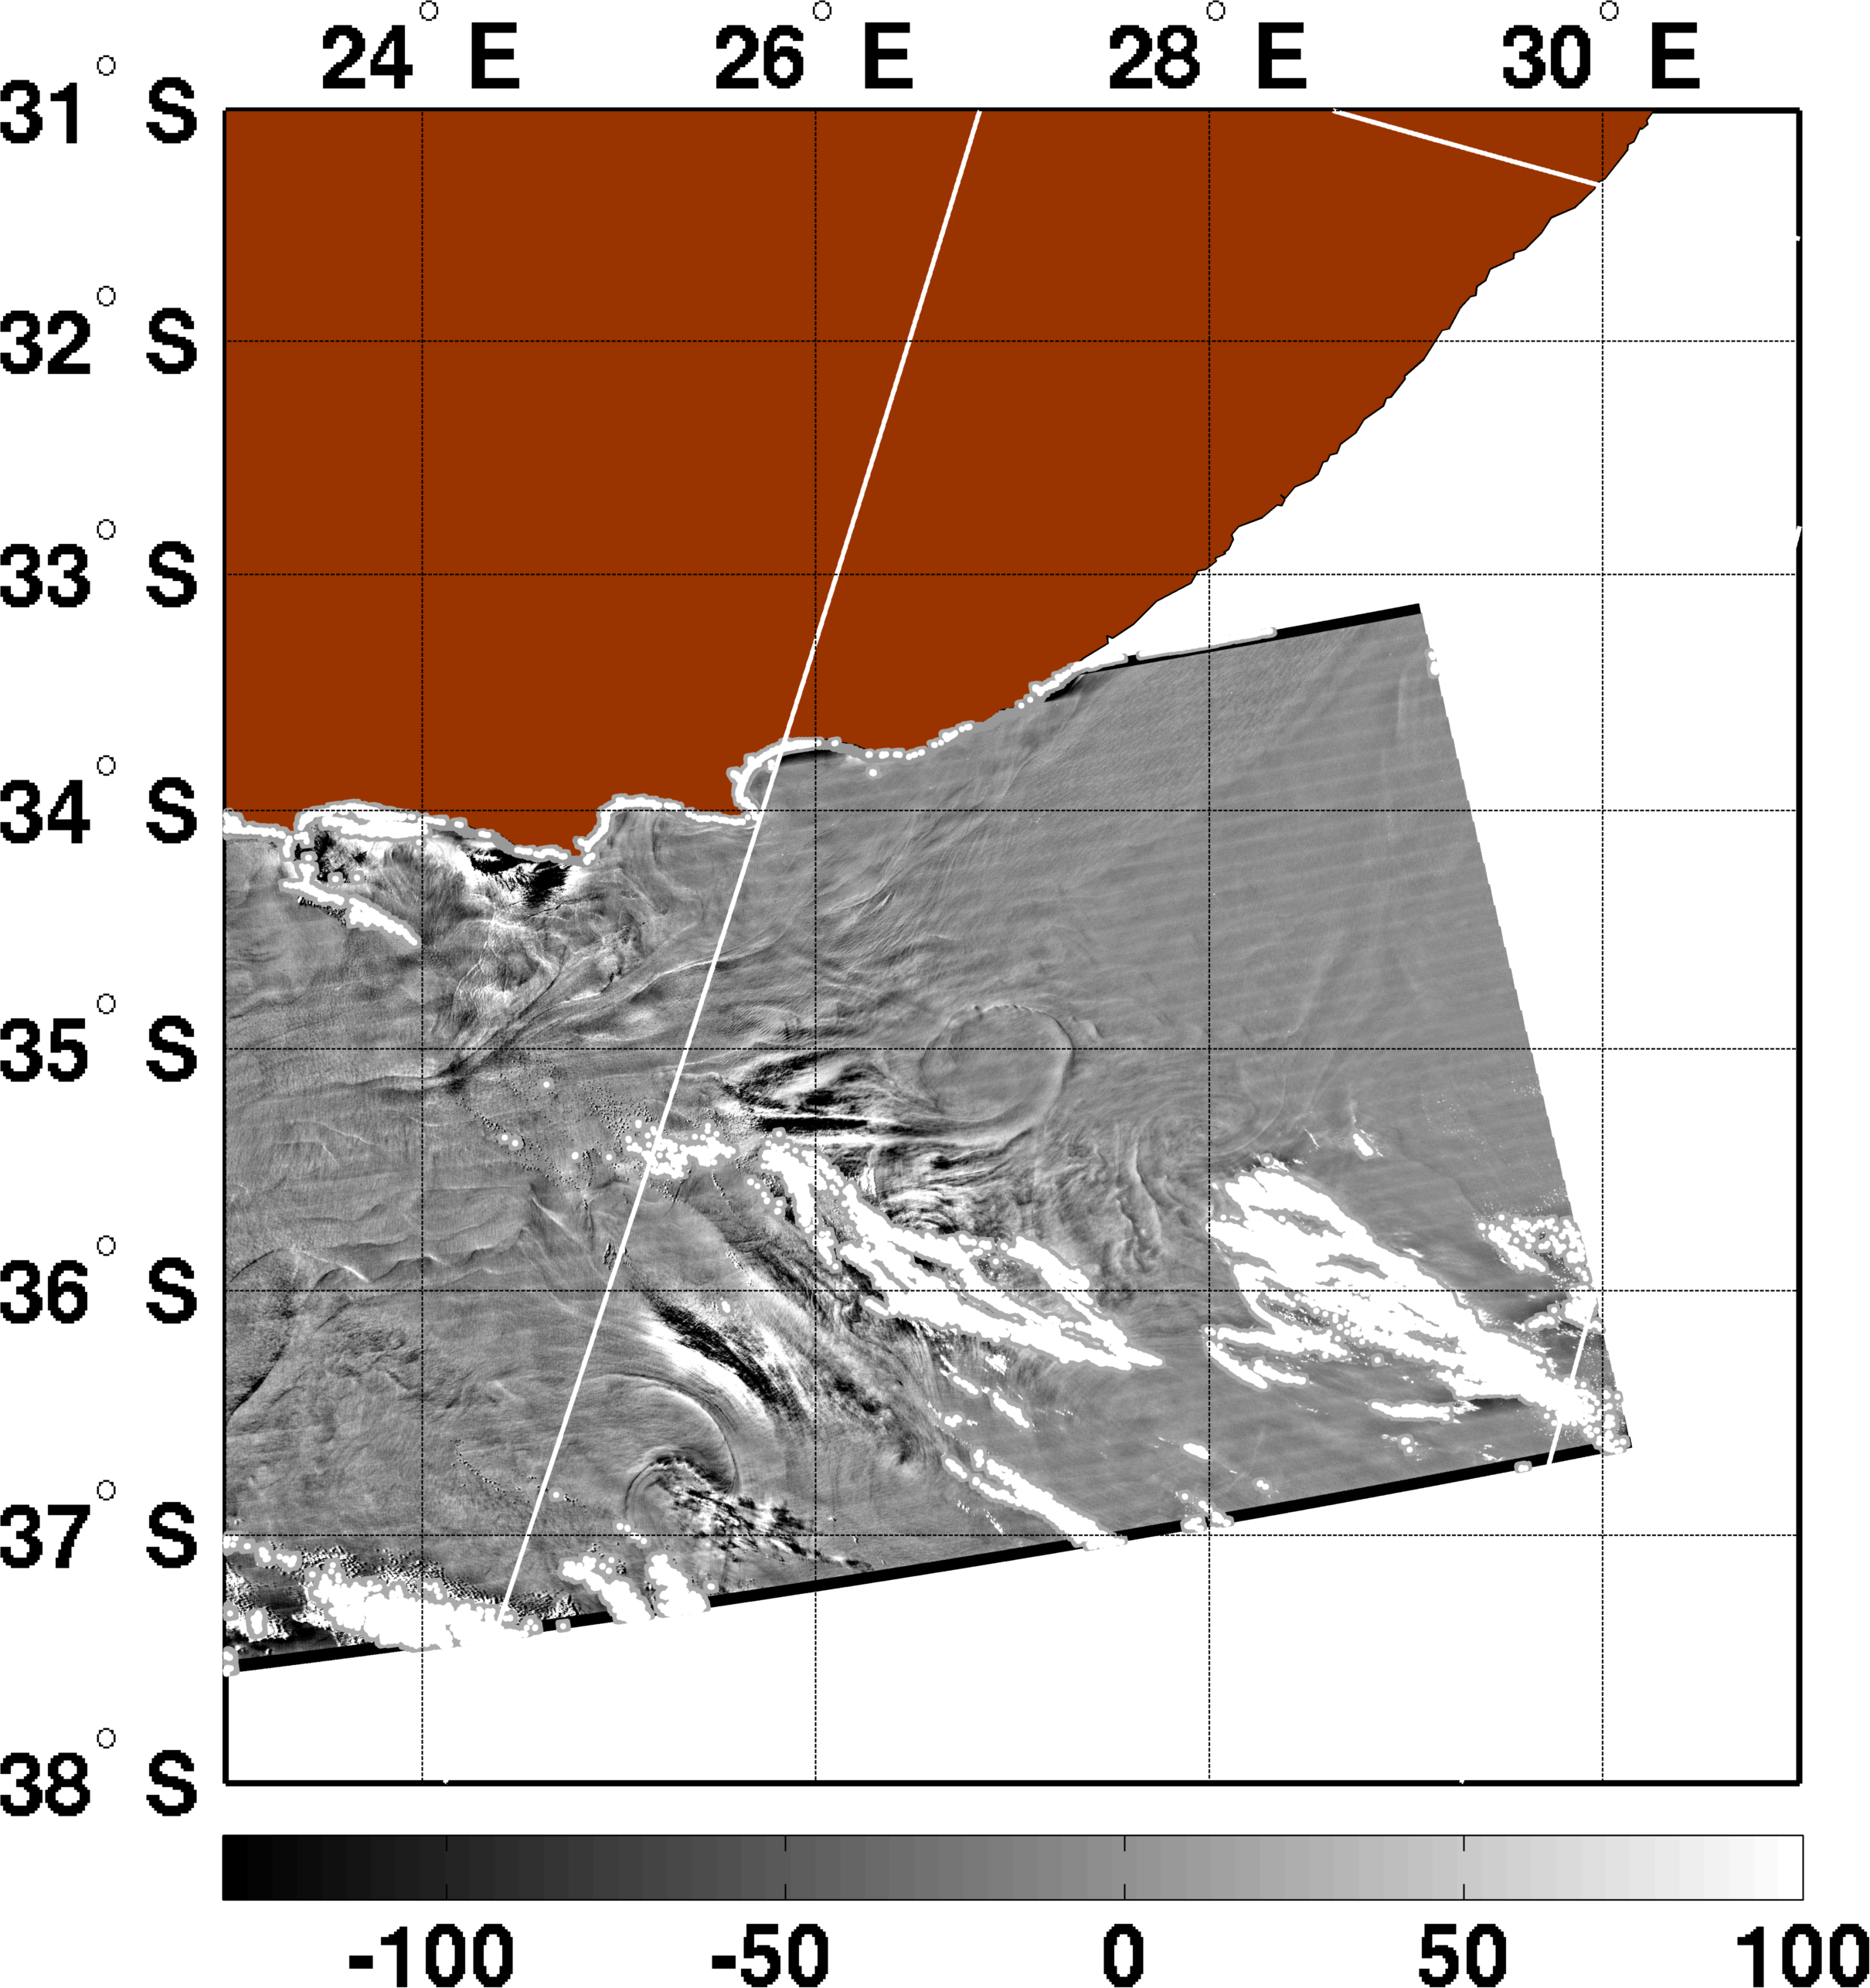
\includegraphics[width=1\linewidth]{fig3_4b}}
	\end{minipage}
    \\
    \floattitle{(а) Исходное изображение MODIS/Aqua района мыса Игольный, красный канал разрешением 250\textit{м}, полученное 18 Ноября 2007г., 12ч. 05мин. и вариации яркости (б). Обратите внимание на полосчатую структуру изображения MODIS, присущую снимкам областей солнечного блика, и особенно заметную на исходном изображении. Белые области -- маска облаков}
    \caption{Исходное изображение MODIS/Aqua района мыса Игольный и восстановленные контрасты СКН}
    \label{fig:3.4}
\end{figure}


На Рисунке~\ref{fig:3.5a} изображены контрасты СКН, полученные из вариаций яркости, приведённых на Рисунке~\ref{fig:3.4b}). Контрасты СКН ``статистически однородны'' на всём районе наблюдения, за исключением локальных областей, покрытых облаками, где отраженная яркость в солнечном блике ``загрязнена'' тенями от облаков и большими значениями яркости отражённой радиации непосредственно от самих облаков. 

Таким образом, в подобных районах, предложенный алгоритм не годен и к восстановленным контрастам СКН стоит относиться с осторожностью. В остальном, метод подчёркивает проявления линейные особенности фронтов, меандров и вихрей. Типичные значения магнитуды контрастов СКН около 20-30\% и масштабами проявления структур от 1 до 10\textit{км}.



\begin{figure}[H]
   	\centering
	\begin{minipage}{.47\textwidth}
	    \subcaptionbox{\label{fig:3.5a}}
		{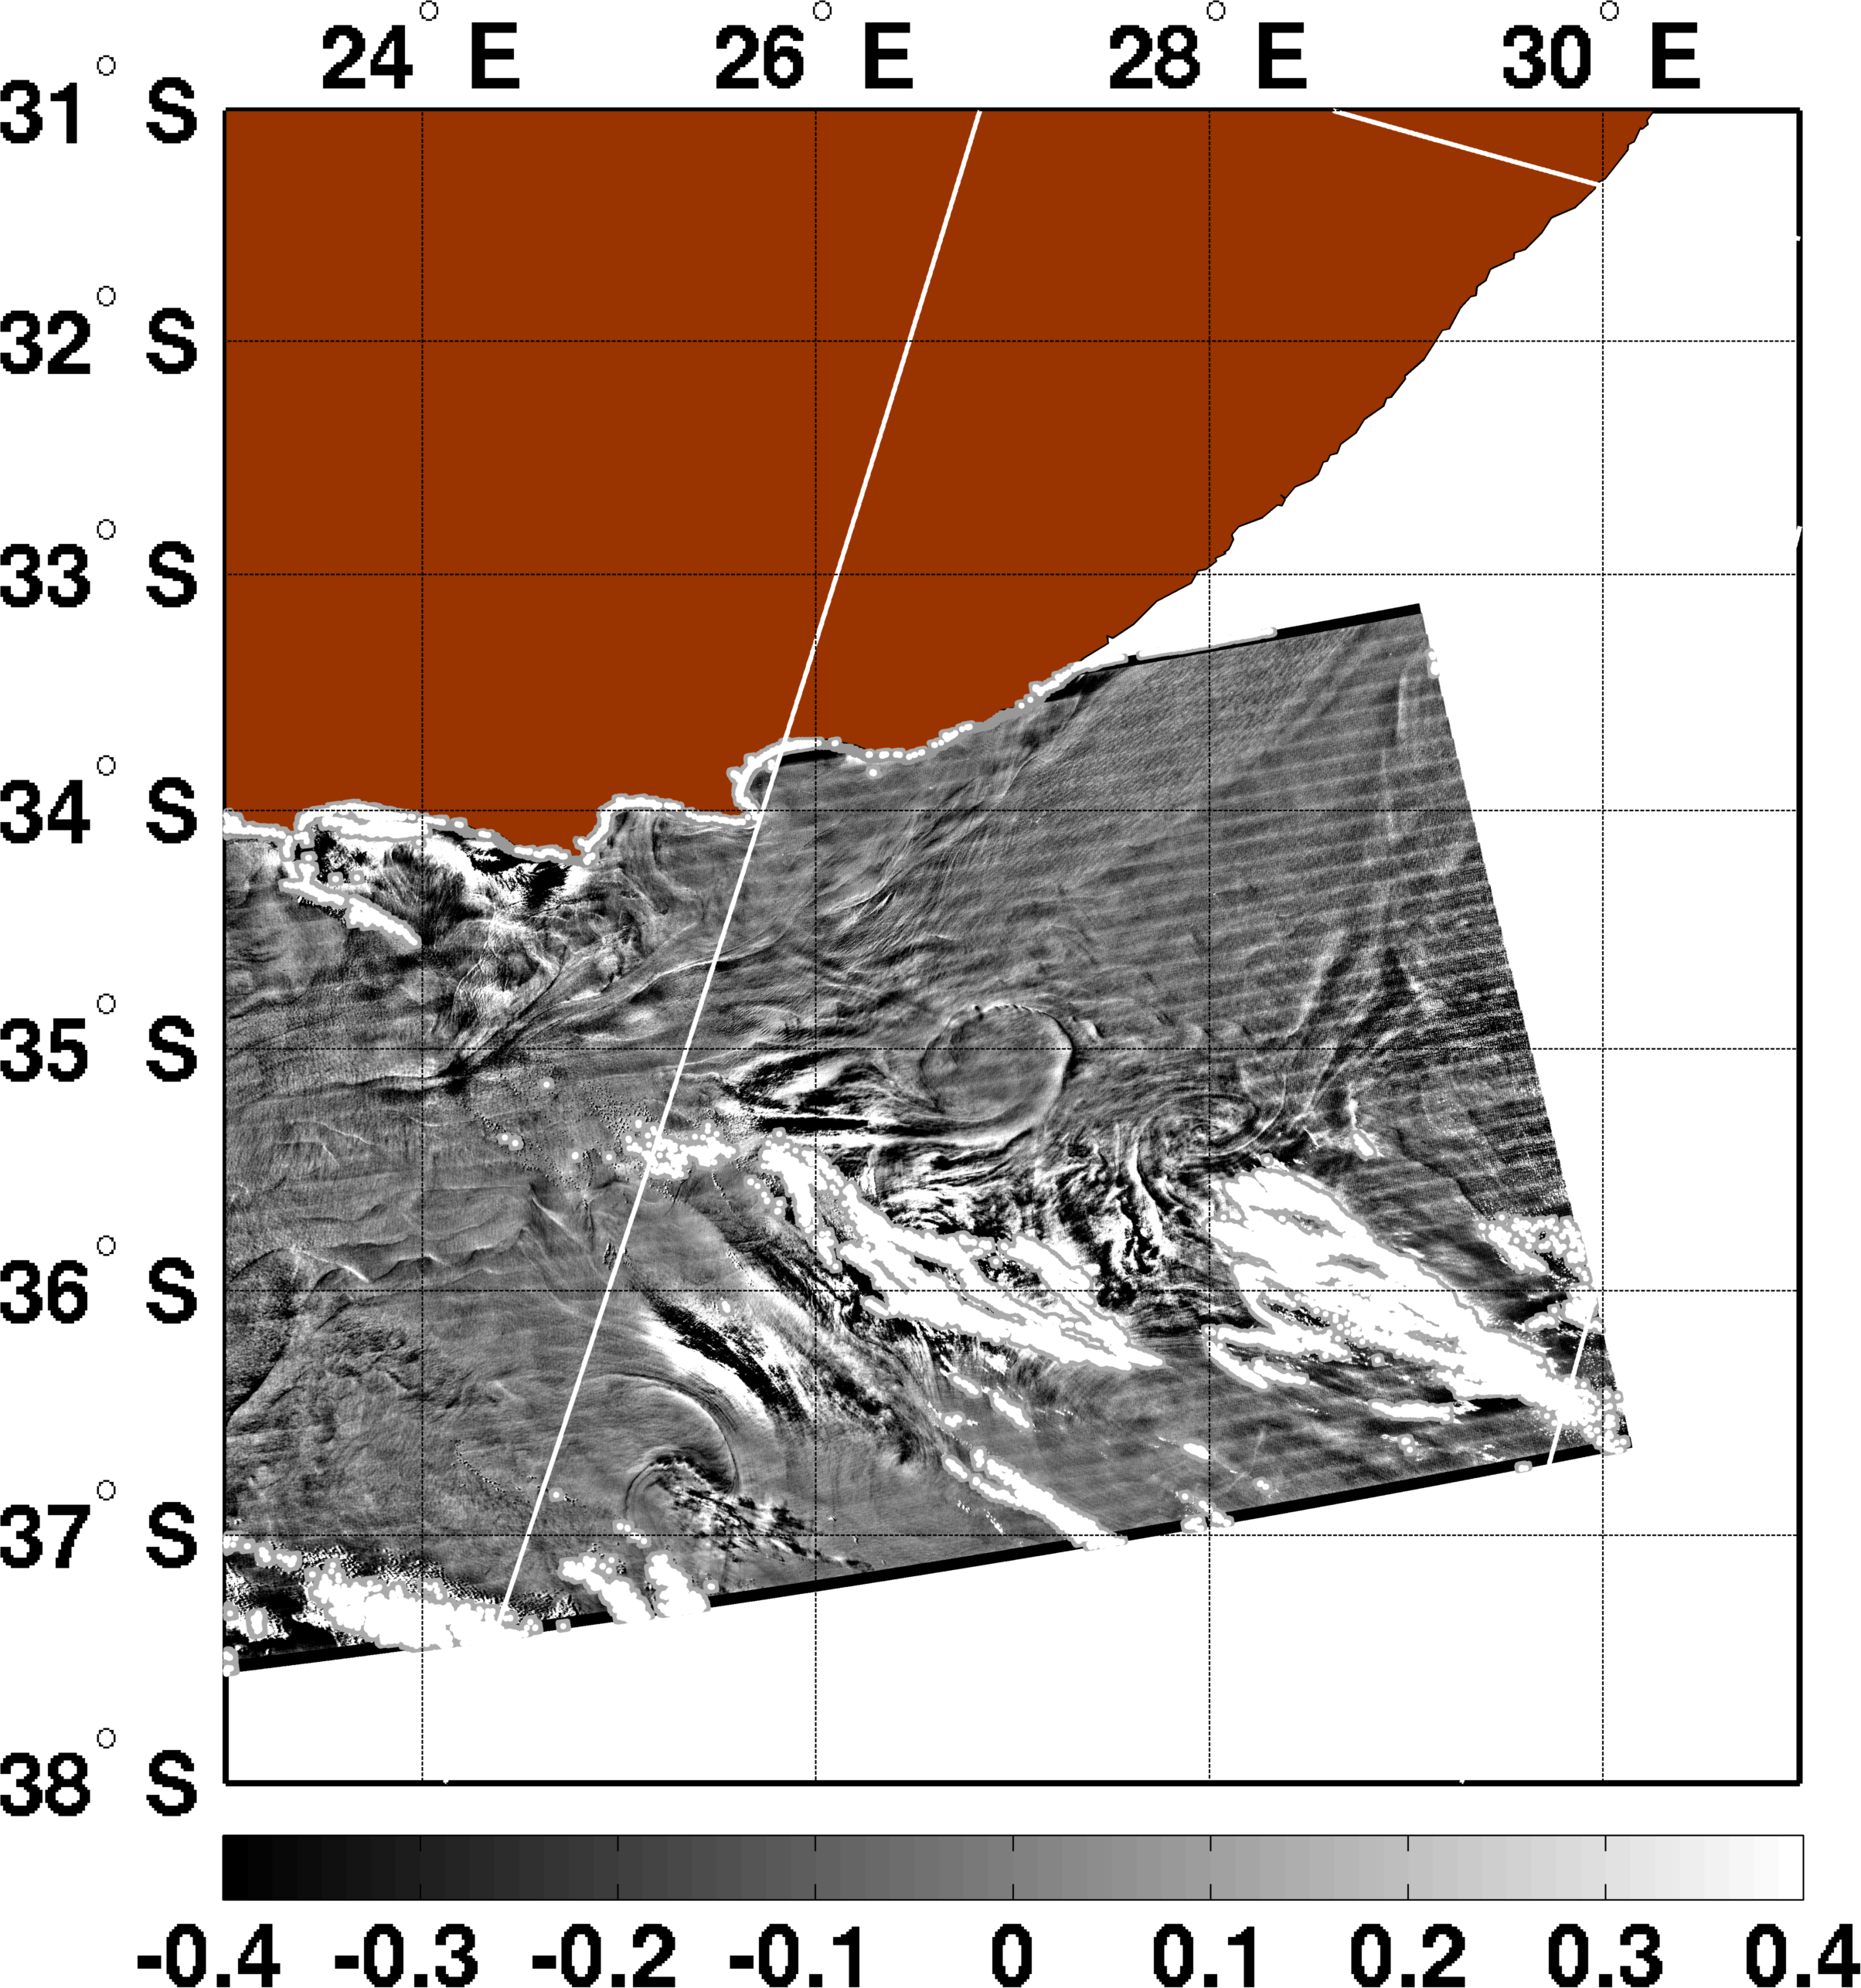
\includegraphics[width=1\linewidth]{fig3_5a}}
	\end{minipage}
	\hfill
	\begin{minipage}{.47\textwidth}
	    \subcaptionbox{\label{fig:3.5b}}
		{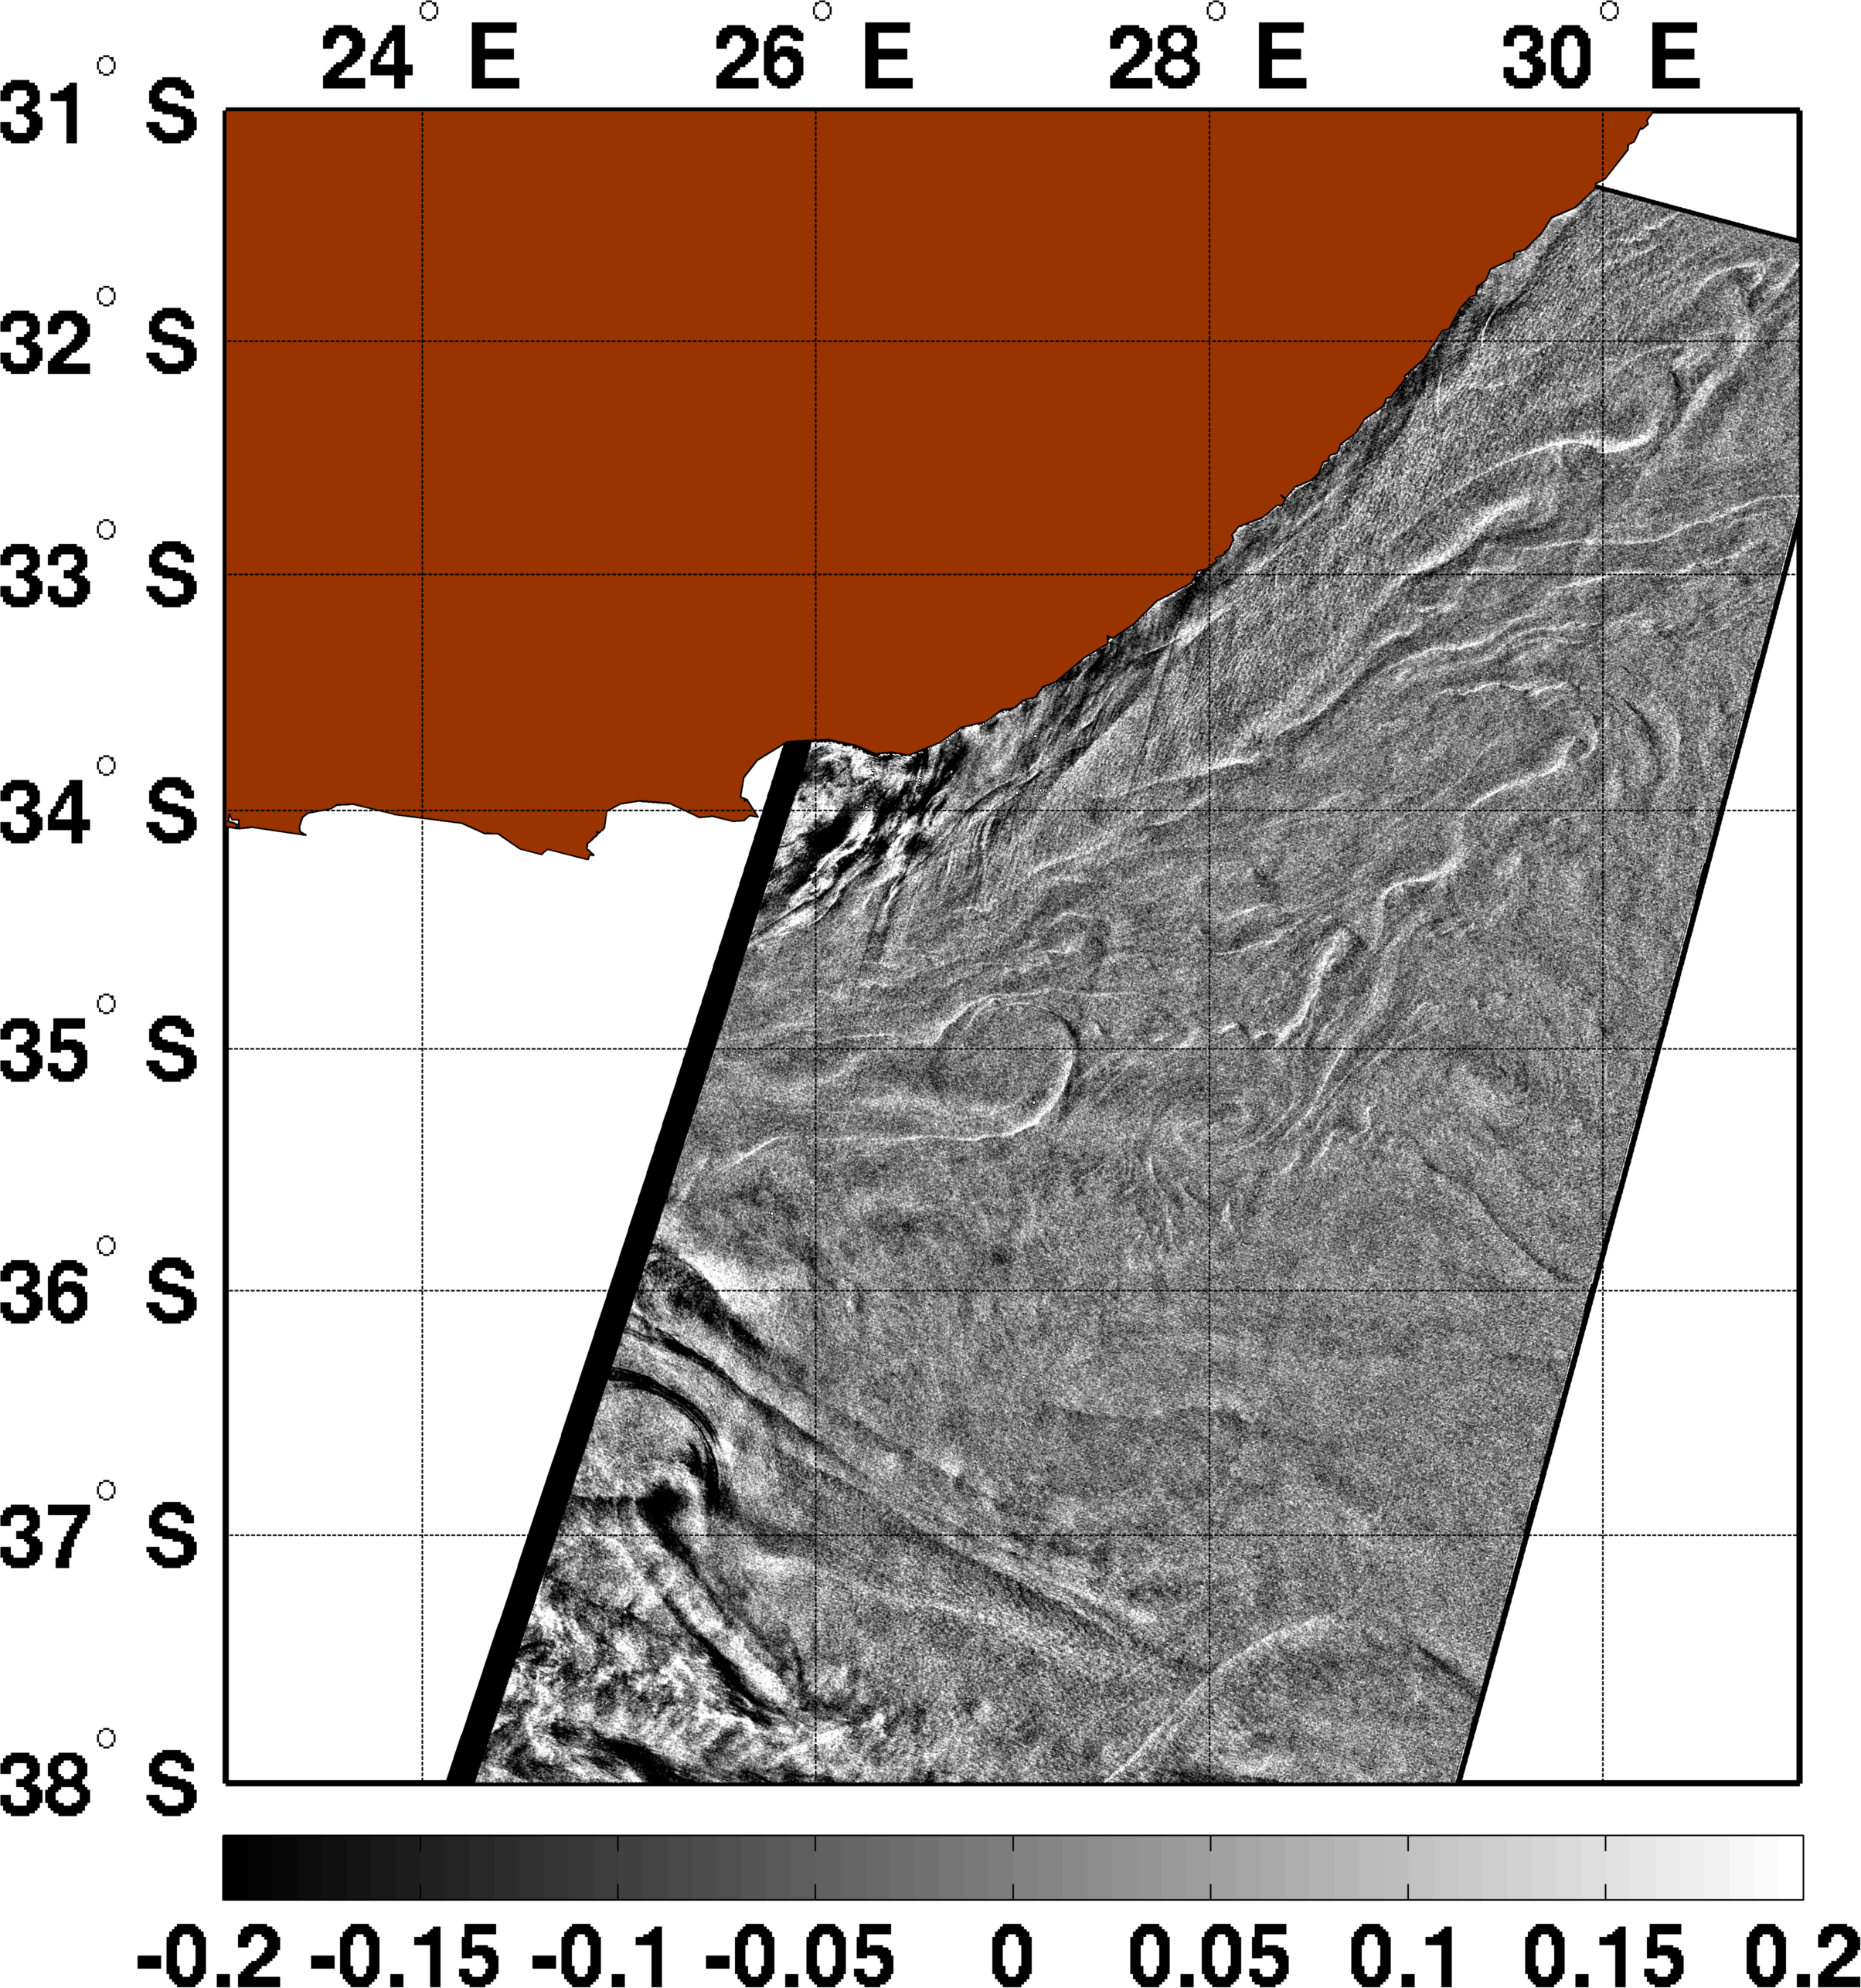
\includegraphics[width=1\linewidth]{fig3_5b}}
	\end{minipage}
    \\
    \caption{(а) Поле контрастов СКН полученное из поля вариаций яркости, представленных на Рисунке~\ref{fig:3.4b} и поле контрастов УЭПР РСА (б)}
    \label{fig:3.5}
\end{figure}


Поле контрастов УЭПР РСА (Рисунок~\ref{fig:3.5b}), $K_{\sigma _{0} } =(\sigma _{0} -\overline{\sigma _{0} })/\overline{\sigma _{0} }$, представлено как отношение разности исходного и осреднённого к среднему полю вариаций УЭПР. Осреднение производилось скользящим средним с пространственным разрешением скользящего окна 30x30\textit{км${}^2$}. При первом же визуальном сравнении поля контрастов СКН и поля контрастов УЭПР РСА наблюдается высокий уровень соответствия между двумя изображениями. Йоханнессен и др. в своей работе обосновали, что особенности на изображения РСА отражают поле дивергенции поверхностного течения. Таким образом, подобие полей контрастов СКН и УЭПР РСА, позволяет утверждать, что поле контрастов СКН также отслеживает поле дивергенции поверхностного течения.



\subsection{Процедура реконструкции квазигеострофической и агеострофической циркуляции по ТПО} \label{sec:3.2.2}


Адвективная составляющая Экмановского переноса и диабатическое перемешивание в Экмановском слое являются одними из основных механизмов генерации вторичной агеострофической циркуляции (ВАЦ), в непосредственной близости от океанических фронтов \citep{Klein1990,Garrett1981,Thompson2000,Nagai2006}. Не так давно обсуждался и другой механизм \citep{McWilliams2009}, выполненный по аналогии с само индуцированным фронтогенезом, для ускорения и обострения температурных фронтов, связанных с исходной ВАЦ. Детальное рассмотрение всех возможных механизмов, безусловно, выходит за рамки настоящего исследования. Тем не менее, чтобы проинтерпретировать совпадающие особенности температурных фронтов и аномалии шероховатости морской поверхности, мы ограничим наш анализ модельным приближением, основываясь на формировании ВАЦ только за счёт первого механизма. Таким образом, мы предполагаем, что полное поле океанического течения можно представить в виде суммы квазигеострофического течения (КГТ) ${\it U}$, ветрового течения ${\it u}^{e} $ (которое также может включать инерционное течение), и ВАЦ ${\it u}^{a} $, в результате взаимодействия Экмановского течения с КГТ и диабатического перемешивания в слое Экмана. Тогда уравнение для полного поля течения выражается как ${\it u=U+u}^{e} {\it +u}^{a} $.

В первом приближении числа Россби, основные уравнения, описывающие динамику течения ВАЦ (подробнее см. \citep{Klein1990,Garrett1981,Thompson2000,Nagai2006}) представляются в виде:



\begin{equation} \label{eq:3.2} \begin{array}{l} {u_{\beta }^{e} \partial U_{1} /\partial x_{\beta } -fu_{2}^{a} =\nu _{t} \partial ^{2} U_{1} /\partial x_{3}^{2} } \\ {u_{\beta }^{e} \partial U_{2} /\partial x_{\beta } +fu_{1}^{a} =\nu _{t} \partial ^{2} U_{2} /\partial x_{3}^{2} } \end{array},  \end{equation} 



\noindent где $\nu _{t} $ - турбулентная вязкость, предполагается постоянной с глубиной (в верхнем перемешенном слое Экмана), $f$ параметр Кориолиса, и$\beta =1,2$. В уравнении \eqref{eq:3.2}, пространственный масштаб изменчивости ветрового поля намного превышает поперечны масштаб фронта. С учётом уравнения сохранения ``термического ветра: $\partial U_{1} /\partial x_{3} =(g/f)\partial \rho /\partial x_{2} $, $\partial U_{2} /\partial x_{3} =-(g/f)\partial \rho /\partial x_{1} $, и уравнения состояния океана $\rho =\rho _{0} (1-\alpha T)$, решение уравнения \eqref{eq:3.2} в терминах ВАЦ даёт



\begin{equation} \label{eq:3.3} \begin{array}{l} {u_{1}^{a} =-f^{-1} u_{\beta }^{e} \frac{\partial U_{2} }{\partial x_{\beta } } +(\nu _{t} g\alpha /f^{2} )\frac{\partial }{\partial x_{3} } \left(\frac{\partial T}{\partial x_{1}^{} } \right)} \\ {u_{2}^{a} =f^{-1} u_{\beta }^{e} \frac{\partial U_{1} }{\partial x_{\beta } } +(\nu _{t} g\alpha /f^{2} )\frac{\partial }{\partial x_{3} } \left(\frac{\partial T}{\partial x_{2}^{} } \right)} \end{array},  \end{equation} 



\noindent где $g$ - ускорение свободного падения, а $\alpha $ - коэффициент термического расширения. Первый член в уравнении \eqref{eq:3.3} описывает генерацию ВАЦ в результате адвективного взаимодействия Экмановского течения с КГТ (механизм предложен \citep{Klein1990}), в то время как второй член учитывает фрикционный эффект в Экмановском слое (механизм описан \citep{Garrett1981}). Оба этих механизма приводят к возникновению дивергенции в окрестности термического фронта, что напрямую следует из уравнения. \eqref{eq:3.3}:



\begin{equation} \label{eq:3.4} \nabla \cdot {\it u}=-f^{-1} u_{\beta }^{e} \frac{\partial }{\partial x_{\beta } } \Omega +(\nu _{t} g\alpha /f^{2} )\frac{\partial }{\partial x_{3} } \Delta T,  \end{equation} 



\noindent где $\Omega _{z} =\partial U_{2} /\partial x_{1} -\partial U_{1} /\partial x_{2} \equiv \Delta \psi $ - завихренность КГТ, $\psi $ - функция тока и $\Delta T$ - Лапласиан поля поверхностной температуры. Соотношение л.ч. уравнения \eqref{eq:3.4} с первым членом его п.ч. представляет решение, полеченное в \citep{Klein1990} для Экмановского адвективного механизма, а уравнение со вторым членом п.ч. уравнения \eqref{eq:3.4} -- решение \citep{Garrett1981}. для диабатического механизма перемешивания при генерации ВАЦ. Таким образом, уравнение \eqref{eq:3.4}, можно рассматривать как обобщённое решение, объединяющее оба механизма генерации ВАЦ в результате взаимодействия КГТ со слоем Экмана.

Для простоты, далее предполагается, что ветровое течение представляется в виде суммы классической скорости течения Экмана ${\it u}^{ek} {\it =}\left[\tau _{2} /(fh),-\tau _{1} /(fh)\right]$ и скорости инерционного течения ${\it u}^{i} (t)$:



\begin{equation} \label{eq:3.5} {\it u}^{e} {\it =}\left[\tau _{2} /(fh),-\tau _{1} /(fh)\right]+{\it u}^{i} (t),  \end{equation} 



\noindent где ${\it \tau }=v_{*}^{2} [\cos \phi _{w} ,\sin \phi _{w} ]$, $v_{*} $ - фрикционная скорость в воде, $\phi _{w} $ - направление вектора скорости ветра, $h=(\nu _{t} /f)^{1/2} $ - глубина слоя Экмана, а инерционная скорость ${\it u}^{i} (t)$ может быть описана, используя временную изменчивость скорости ветра. Выражение для турбулентной вязкости $\nu _{t} $ следует из сходства морского и атмосферного пограничного (планетарного) слоя Экмана. Для устойчиво стратифицированного пограничного слоя турбулентная вязкость $\nu _{t} =\gamma \kappa v_{*}^{} L$, где $\gamma \approx 0.2$ - постоянная, $\kappa \approx 0.4$ - постоянная Кармана, а $L$ - масштаб длины Обухова (см., например, \citep{Brown1982}). Выражая $L$ через частоту Брента-Вяйсяля для верхнего слоя океана как $L=v_{*}^{3} /(\kappa v_{t} N^{2} )$, получаем турбулентную вязкость:



\begin{equation} \label{eq:3.6} \nu _{t} =\gamma ^{1/2} v_{*}^{2} /N,  \end{equation}



\noindent тогда глубина слоя Экмана:



\begin{equation} \label{eq:3.7} h=\gamma ^{1/4} v_{*} /\sqrt{fN} .  \end{equation} 



Оценка $h$ для скорости ветра 10\textit{м/с} и $f=10^{-4} $: $h\approx 28$\textit{м}, если соотношение Прандтля $N/f=10$, и $h\approx 90$\textit{м}, если $N/f=1$.

Чтобы дать определение дивергенции поверхностного течения (вызванную ВАЦ, в соответствии с уравнением \eqref{eq:3.4}), необходимо ввести поле КГТ. На мезомасштабах (10-500км) и субмезомасштабах (1-10km), динамика океана такова, что, зачастую, в равновесно стратифицированном, быстро вращающемся потоке горизонтальные скорости, в среднем, значительно больше вертикальных. Таким образом, такое движение можно рассматривать как квази-двумерное, и его изучение проводить в рамках некоторых приближений. Основываясь на поверхностной квазигеострофической (ПКГ, от англ. SQG) динамике \citep{Held1995,Lapeyre2006}, Изерн-Фонтанет с коллегами \citep{Isern-Fontanet2008} предложили практический подход для восстановления поля скорости течения на масштабах от 30 до 300 километров по изображению ТПО. Рассматривая ПКГ, функция тока КГТ $\widehat{\psi }({\it k},z)$ поле ТПО $\widehat{T}_{s} ({\it k})$ в пространстве Фурье связаны следующим соотношением:



\begin{equation} \label{eq:3.8} \widehat{\psi }({\it k},z)=\frac{g\alpha \widehat{T}_{s} ({\it k})}{fn_{b} k} \exp (n_{0} kz),  \end{equation} 



\noindent где $n=N/f$ отношение Прандтля для частот Брента-Вяйсяля $N_{0} $ и $N_{b} $, определяющих, соответственно, мезо- и субмезомасштабные свойства потока. Определяя скорость КГТ через функцию тока $\widehat{\psi }$, как $\widehat{{\it U}}=(-ik_{y} \widehat{\psi },ik_{x} \widehat{\psi })$ (или в физическом пространстве ${\it U}=(-\partial \psi /\partial x_{2} ,\partial \psi /\partial x_{1} )$), тогда, используя уравнение \eqref{eq:3.3}, возможно определить поле ВАЦ. 

В пространстве Фурье, компоненты ВАЦ, определённые уравнениями \eqref{eq:3.3} и \eqref{eq:3.8}, и, дополненные оценками глубины слоя Экмана, по уравнению \eqref{eq:3.7} и коэффициентом турбулентной вязкости из уравнения \eqref{eq:3.6}, выражаются через ТПО как:



\begin{equation} \label{eq:3.9} \left(\widehat{u_{1}^{a} },\widehat{u_{2}^{a} }\right){\rm =}\frac{\alpha }{\gamma ^{1/4} n_{b}^{1/2} } \cdot \frac{gv_{*} }{f^{2} } \left[s\cdot \sin (\phi _{w} -\phi )+i\gamma ^{3/4} n_{b}^{1/2} \frac{v_{*} K}{\left|f\right|} \right]\left(K_{1} ,K_{2} \right)\widehat{T}_{s} ,  \end{equation} 



\noindent где $s={\rm sign}(f)$, $i$ - мнимая единица, $\phi $ - направление вектора волнового числа ${\it K}$, и $\gamma =0.2$, как и в предыдущих уравнениях. Второй член в квадратных скобках отражает значимость отношения механизма перемешивания к адвективному члену. Если предположить, что $n_{b} =10$ и $f=10^{-4} $сек-1, тогда это отношение будет приблизительно равно 0.1 для скорости ветра 10\textit{м/с} и $K=2\pi /10^{4} $\textit{рад/м}. Для сравнения, это отношение приближается к единице для меньших масштабов, например, $K=2\pi /10^{3} $\textit{рад/м}. Эффективность механизма перемешивания возрастает как при уменьшении масштабов КГТ, так и при увеличении скорости ветра. Таким образом, при малых и умеренных скоростях ветра и масштабах течения порядка $K\propto 10^{-3} $\textit{рад/м} и меньших, механизма Экмановского переноса (который в общем случае также включает инерционные течения) доминирует над генерацией ВАЦ. Из уравнения \eqref{eq:3.9}, получаем выражение для дивергенции поверхностного течения в пространстве Фурье $\widehat{\nabla \cdot {\it u}}=iK_{\beta } \widehat{u_{\beta }^{a} }$:



\begin{equation} \label{eq:3.10} \widehat{\nabla \cdot {\it u}}{\rm =}\frac{i\alpha }{\gamma ^{1/4} n_{b}^{1/2} } \cdot \frac{gv_{*} }{f^{2} } \left[s\cdot \sin (\phi _{w} -\phi )+i\gamma ^{3/4} n_{b}^{1/2} \frac{v_{*} K}{\left|f\right|} \right]K^{2} \widehat{T}_{s} .  \end{equation} 



В результате перед нами уравнение, напрямую связывающее дивергенцию поверхностного течения с полем ТПО.



\subsection{Особенности мезомасштабных течений, восстановленные по ТПО, и их связь с аномалиями РСА сигнала и СКН} \label{sec:3.2.3}
 

Продолжим анализ данных, представленных в разделе \ref{sec:3.2.1}. Сравнивая шероховатость СКН и особенности в УЭПР (показанные на Рисунке~\ref{fig:3.5}) с паттернами в поле ТПО (представлены на Рисунке~\ref{fig:3.3} ), поражает удивительное качественное соответствие этих полей. Основные изменения шероховатости поверхности совпадают с локальными фронтами ТПО. В принципе, эти наблюдения не должны удивлять, поскольку известно, что океанические фронтальные зоны характеризуются интенсивными перекрестными фронтальными и вертикальными движениями (апвеллинг/даунвеллинг). В этом контексте, может быть использована модель восстановления поля поверхностных течений по изображению поля ТПО, в качестве дополнительного экспериментального свидетельства связи между аномалией шероховатости морской поверхности и полем дивергенции течения.

Поле ТПО, полученное по данным прибора MODIS (см. Рисунок~\ref{fig:3.3b} ) и поле, восстановленного по данным РСА, ветра (см. Рисунок~\ref{fig:3.3a} ) используются далее в качестве входных параметров для нахождения поля скорости поверхностного течения. Чтобы избавиться от крупномасштабной изменчивости ТПО, были отфильтрованы спектральные компоненты с $K<2\pi /100$\textit{рад/км}. Спектральное преобразование функции тока КГТ определено из уравнения \eqref{eq:3.8}, предполагая $n_{b} =n_{0} =50$. Стандартное отклонение полученных скоростей КГТ составляет около 1\textit{м/с}. Использование этих констант также помогает сравнивать полученные по РСА поверхностные скорости \citep{Chapron2005, Johannessen2008} с измерениями Доплеровских сдвигов по дальности (не показано здесь). Фоновое Экмановское течение, уравнение \eqref{eq:3.5}, и ВАЦ, уравнение \eqref{eq:3.3}, рассчитаны для ``среднего наблюдаемого'' ветра, южного по направлению, и дующего со скоростью 7\textit{м/с}.

Завихренность поля КГТ и дивергенция поверхностного течения, восстановленные по наблюдаемому полю ТПО, показаны на Рисунке~\ref{fig:3.6}. Поле завихренности КГТ демонстрирует разнообразие мезомасштабных паттернов и наличие ``основной струи'', представляющей течение мыса Игольный. При сравнении с дивергенцией поверхностного течения, можно обнаружить, что паттерны конвергенции/дивергенции повторяют градиенты поля завихренности КГТ, которое, в свою очередь, схоже с полем Лапласиана ТПО.



\begin{figure}[H]
   	\centering
	\begin{minipage}{.47\textwidth}
	    \subcaptionbox{\label{fig:3.6a}}
		{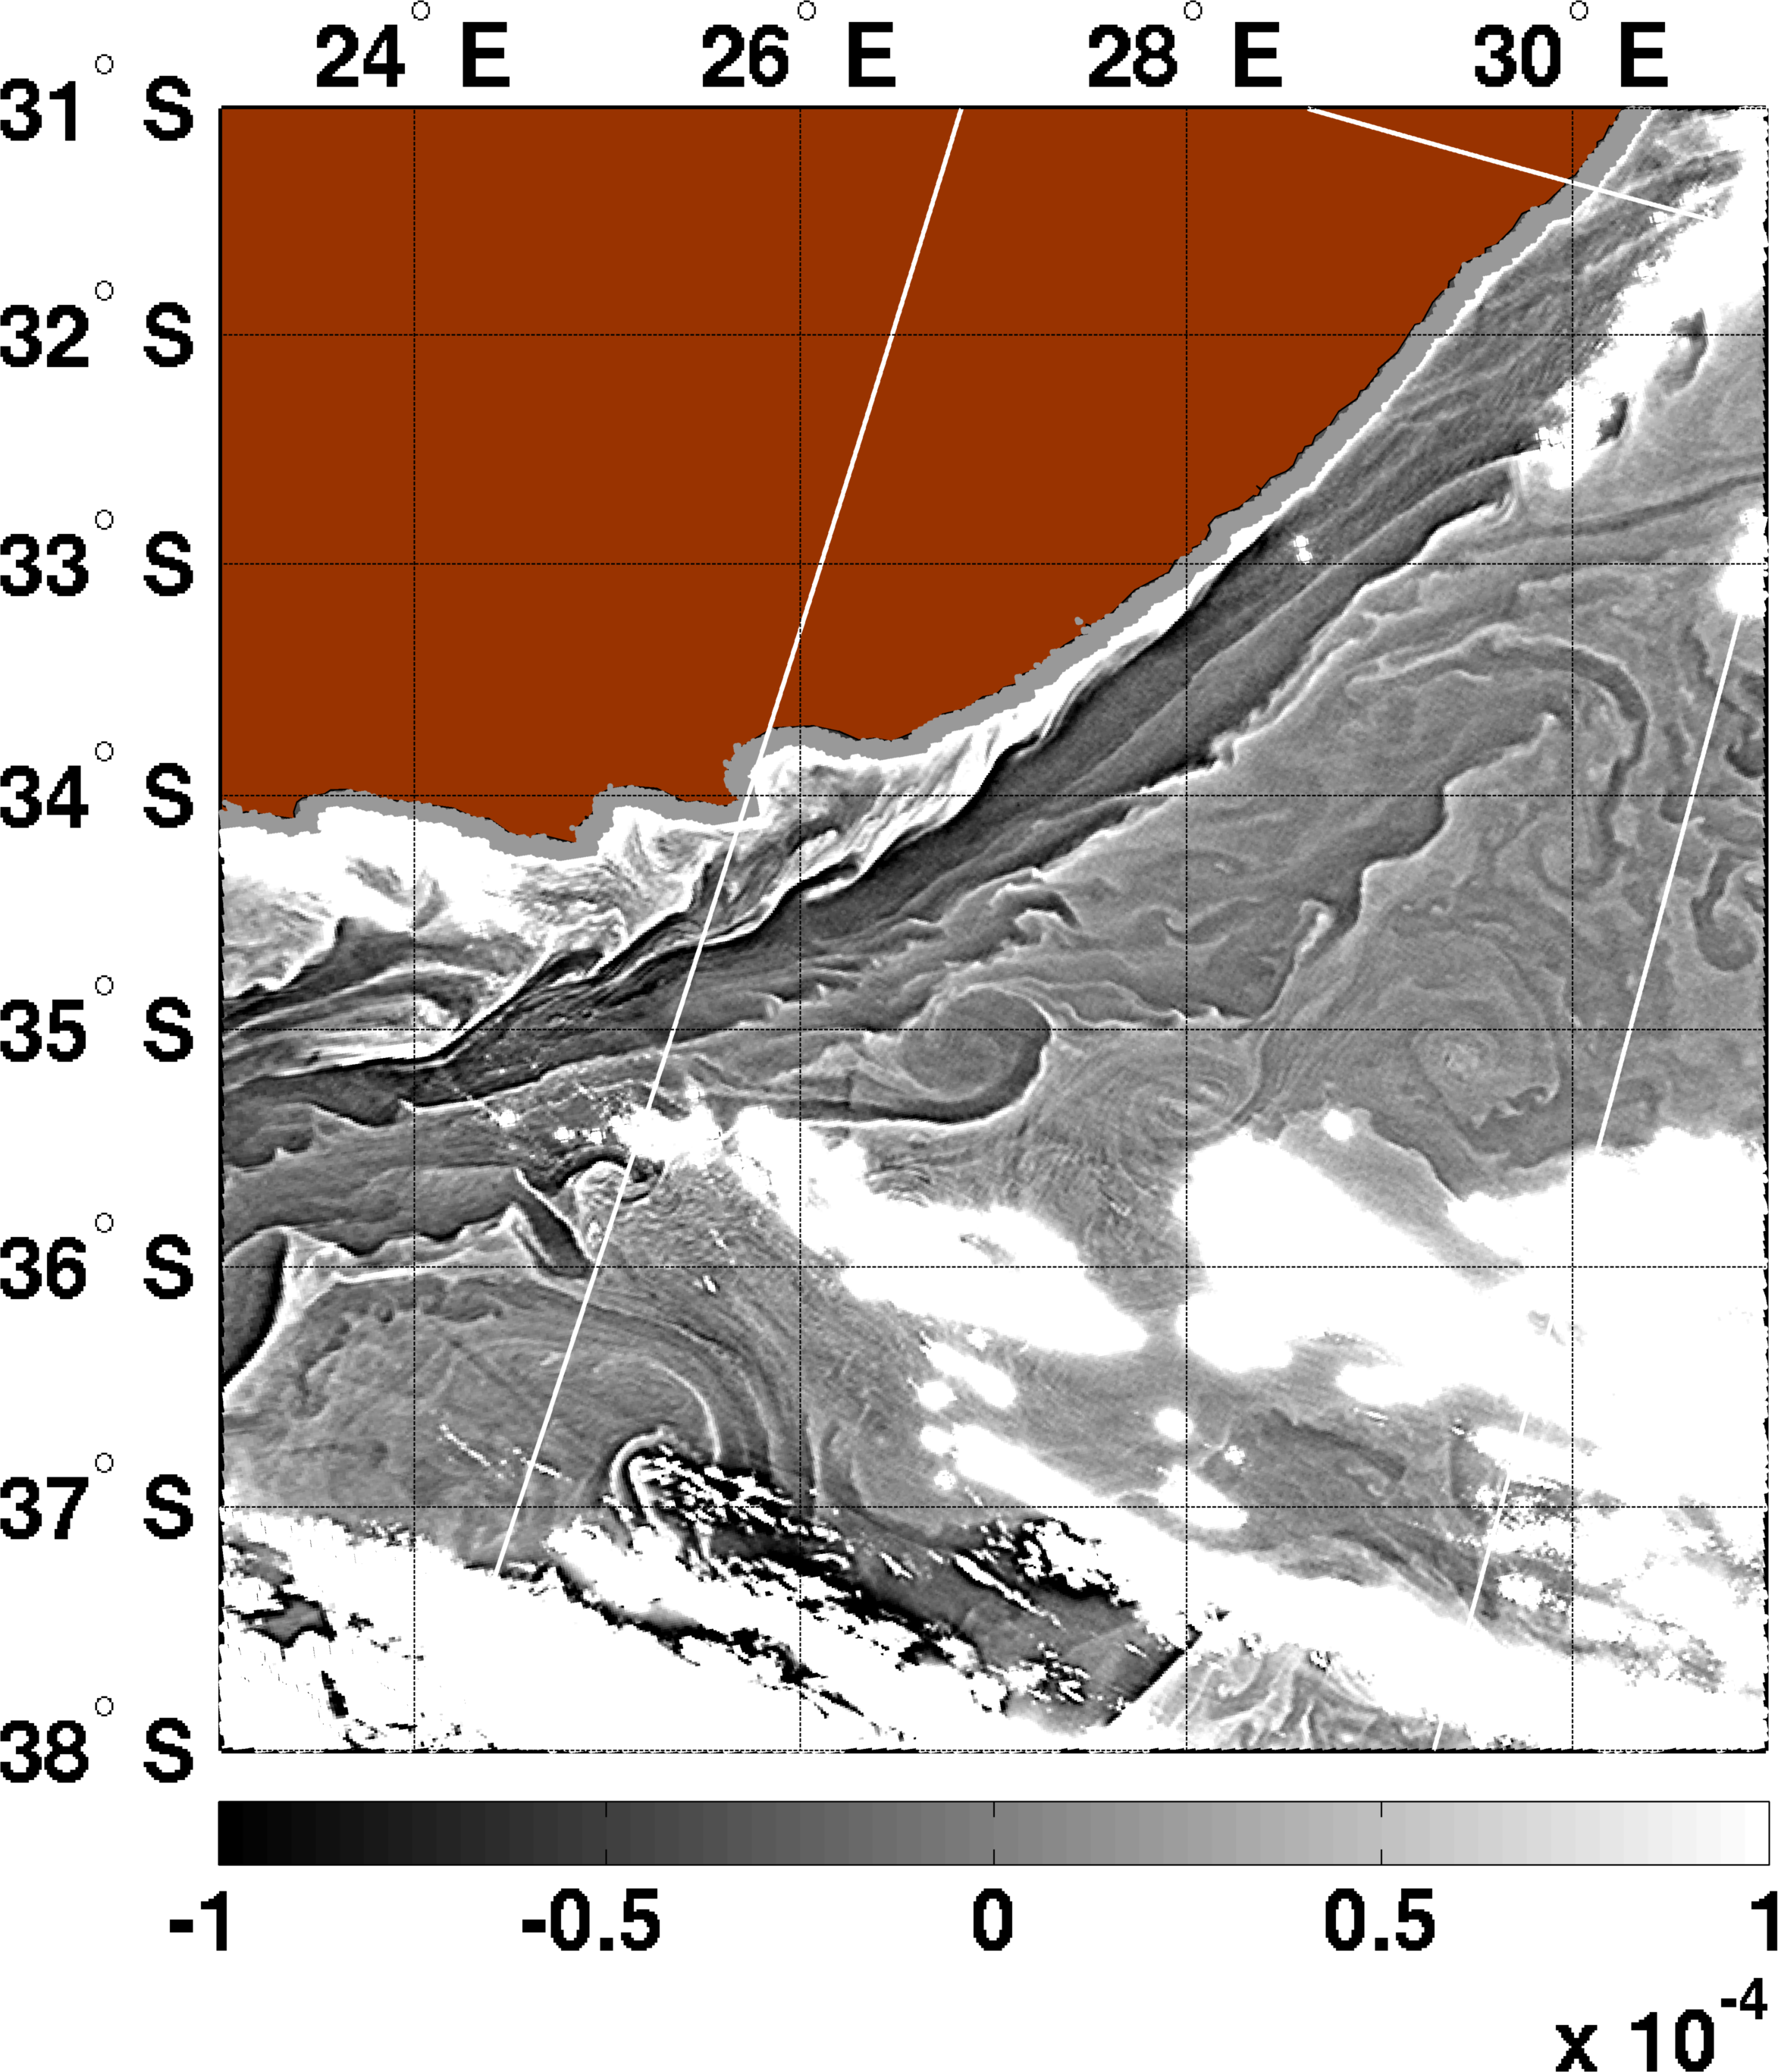
\includegraphics[width=1\linewidth]{fig3_6a}}
	\end{minipage}
	\hfill
	\begin{minipage}{.47\textwidth}
	    \subcaptionbox{\label{fig:3.6b}}
		{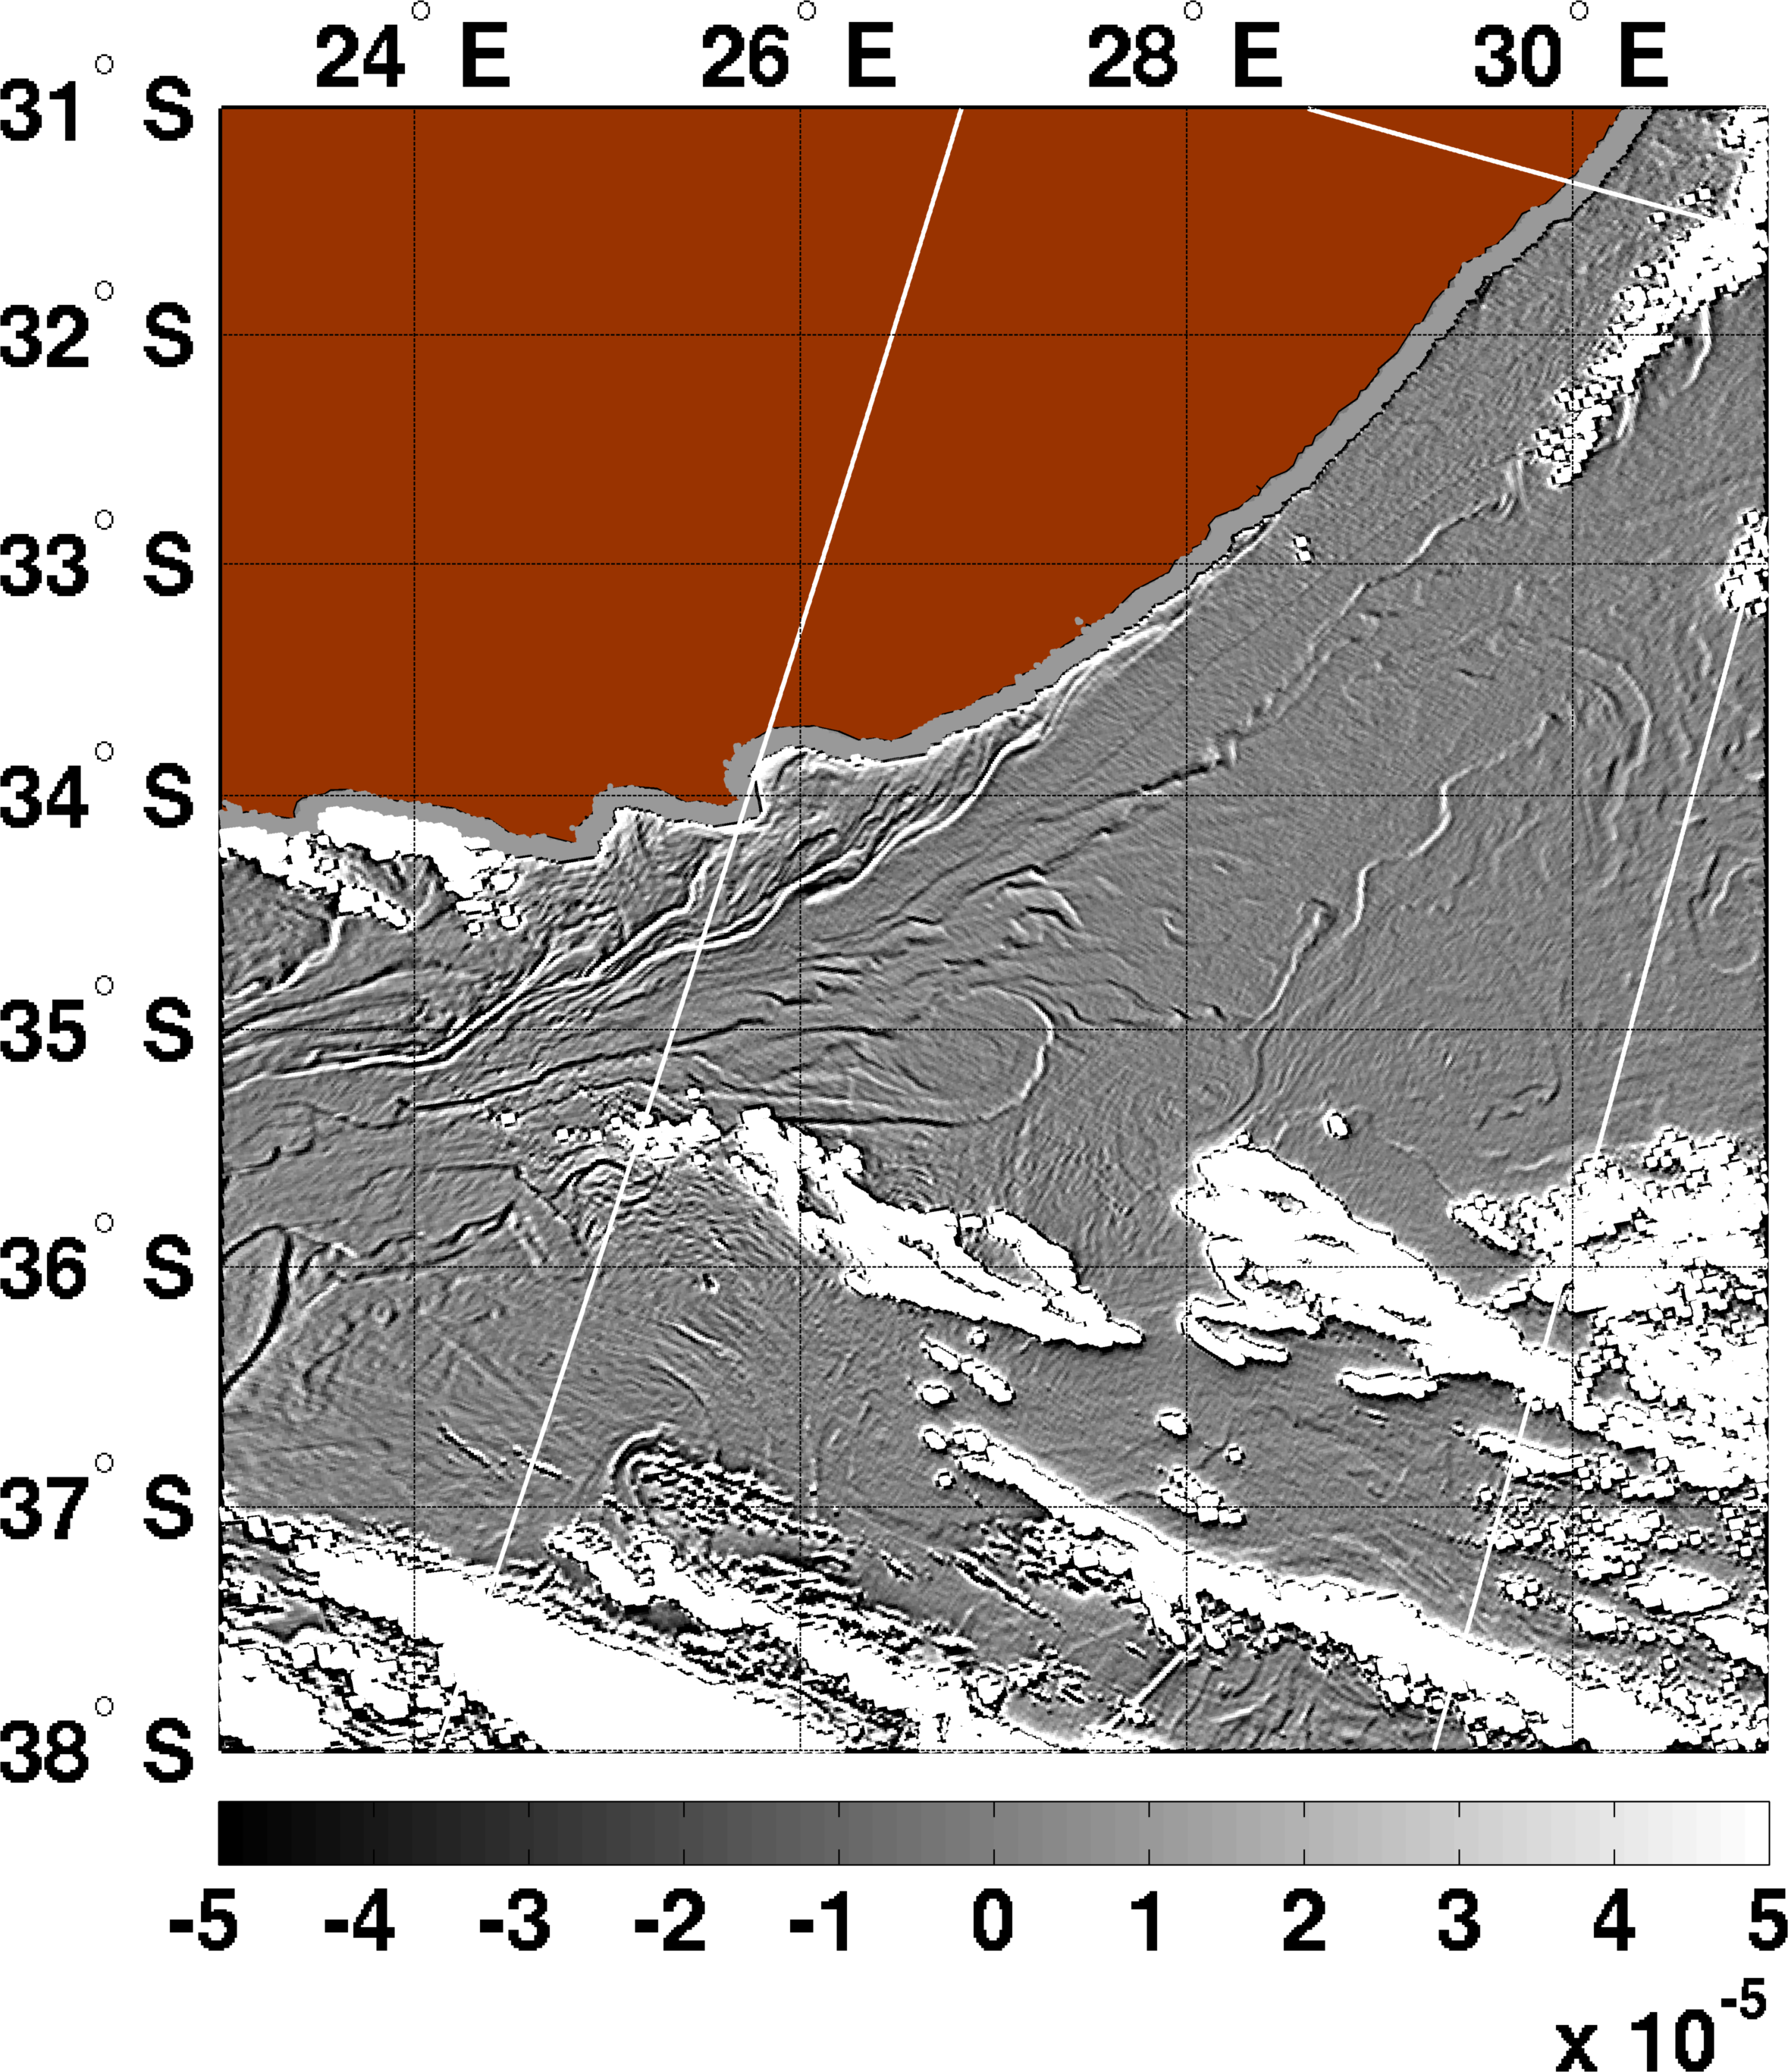
\includegraphics[width=1\linewidth]{fig3_6b}}
	\end{minipage}
    \\
    \floattitle{(а) Завихренность поверхностного квазигеострофического течения (КГТ), полученное по полю ТПО, показанному на Рисунке~\ref{fig:3.3b} , используя уравнение. (б) Поле поверхностной дивергенции, $\nabla \cdot {\it u}$, относящееся ко вторичной агеострофической циркуляции, образующейся в результате взаимодействия Экмановской накачки (адвективный и механизм перемешивания) с КГТ (см. уравнения \eqref{eq:3.4} и \eqref{eq:3.10}). Стоит отметить, что поле дивергенции инвертировано (показано поле $-\nabla \cdot {\it u}$). Таким образом, яркие объекты на изображении соответствуют зонам конвергенции, а тёмные -- зонам дивергенции}
    \caption{Завихренность поля КГТ и дивергенция поверхностного течения, восстановленные по наблюдаемому полю ТПО}
    \label{fig:3.6}
\end{figure}


Присмотревшись к фрагменту РСА изображения на Рисунке~\ref{fig:3.7a} (соответствующее области севернее 36${}^\circ$ Ю.Ш. на Рисунке~\ref{fig:3.5}), где, предположительно, поле ветра однородно, изображенные РСА контрасты можно трактовать как поверхностные проявления мезомасштабной динамики океана. Соответствующее поле дивергенции поверхностного течения представлено на Рисунке~\ref{fig:3.7b}. 



\begin{figure}[H]
   	\centering
	\begin{minipage}{.47\textwidth}
	    \subcaptionbox{\label{fig:3.7a}}
		{\includegraphics[width=1\linewidth]{fig3_7a}}
	\end{minipage}
	\hfill
	\begin{minipage}{.47\textwidth}
	    \subcaptionbox{\label{fig:3.7b}}
		{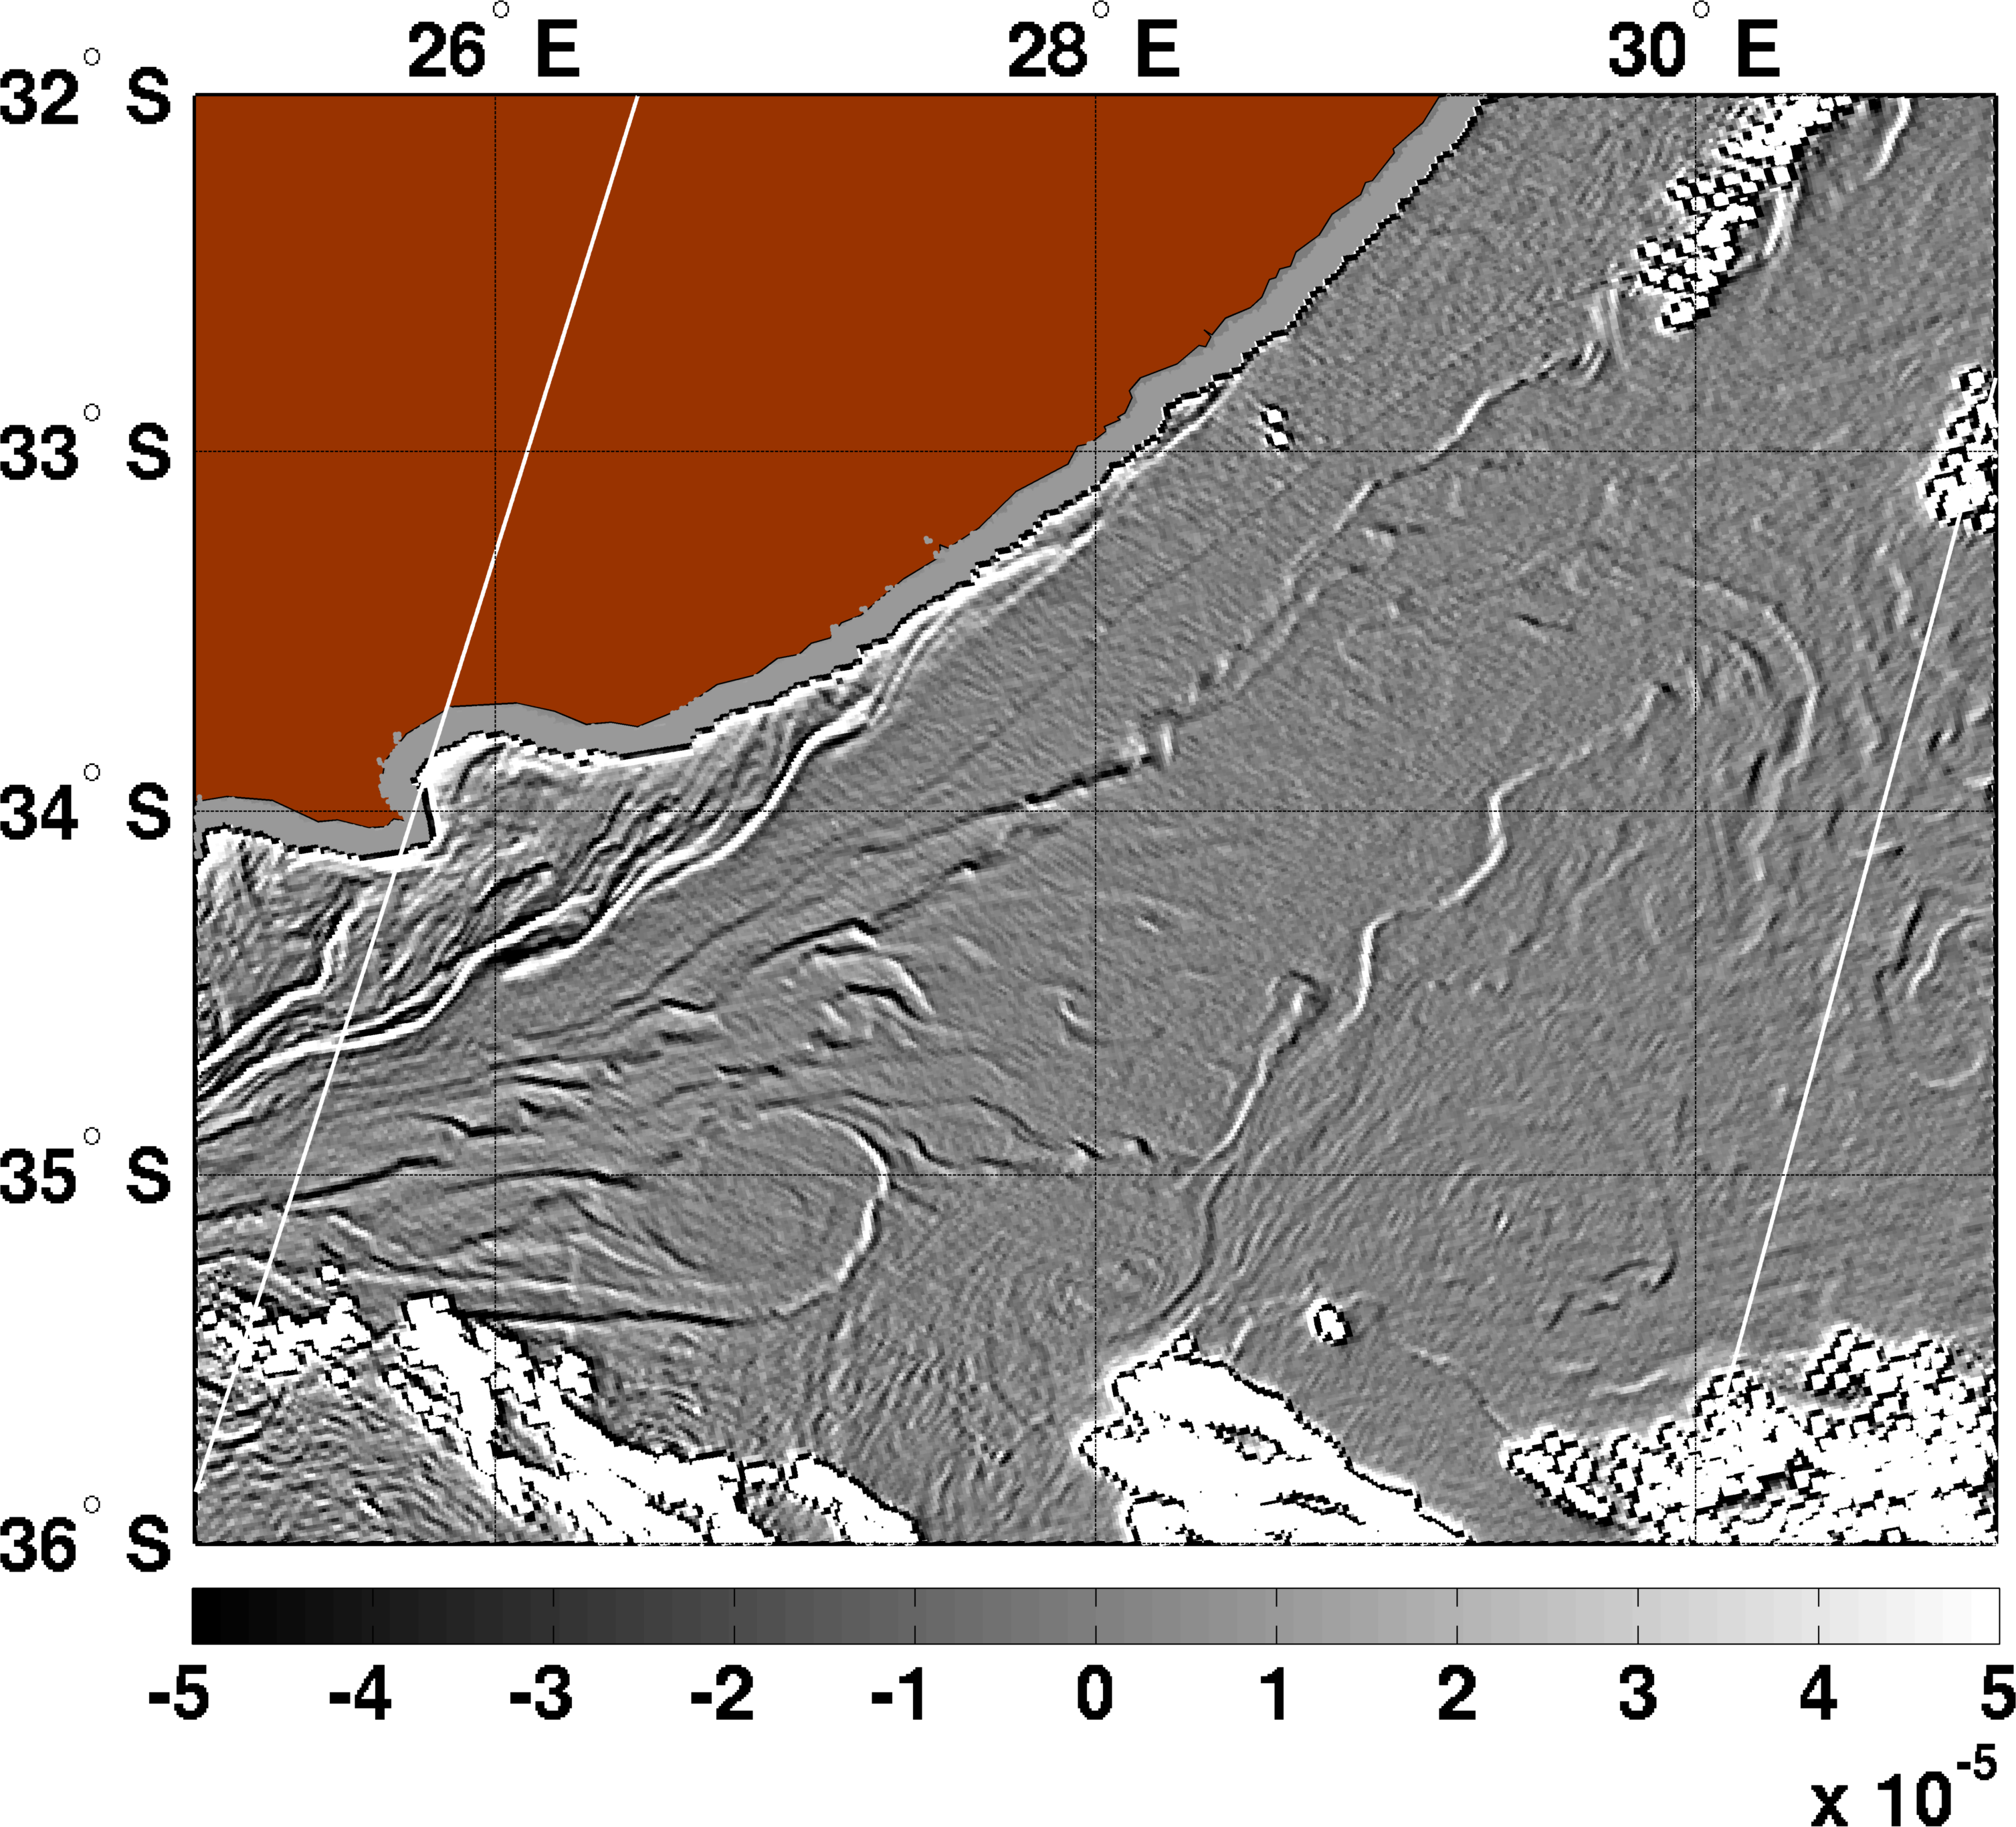
\includegraphics[width=1\linewidth]{fig3_7b}}
	\end{minipage}
    \\
    \floattitle{(а) Фрагмент поля УЭПР РСА, показанный ранее на Рисунке~\ref{fig:3.5}, и (б) соответствующий фрагмент поля дивергенции поверхностного течения, показанного на Рисунке~\ref{fig:3.6}. Яркие области на рисунке (б) соответствуют конвергенции течения, а тёмные -- дивергенции (детальнее см. подпись к Рисунку~\ref{fig:3.6})}
    \caption{Фрагменты поля УЭПР РСА и дивергенции поверхностного течения}
    \label{fig:3.7}
\end{figure}


Визуальный осмотр изображений на Рисунке~\ref{fig:3.7} показывает, что поля контрастов УЭПР и дивергенции имеют очень похожие текстуры. При этом не стоит забывать о 5-и часовой разнице при получении изображениями ASAR и MODIS. В общем и целом, яркие контрасты УЭПР соответствуют зонам конвергенции течения, в то время как тёмные контрасты представляют области дивергенции. Более того, это наблюдение можно рассматривать как экспериментальное подтверждение модельных открытий, представленных в работах \citep{Kudryavtsev2005,Johannessen2005}, и, упрощенных в уравнениях \eqref{eq:1.5}, \eqref{eq:1.7}, \eqref{eq:1.8} и \eqref{eq:1.9}. Также, если существует связь между аномалиями УЭПР и дивергенцией течения, то явное хорошее соответствие между отклонениями РСА контрастов и полем дивергенции поверхностного течения означает, что наш подход для восстановления КГТ и ВАЦ работает должным образом и дает правдоподобные оценки поля поверхностного течения.

Аналогичный вывод может быть сделан для фрагмента поля контрастов СКН, изображенного на Рисунке~\ref{fig:3.8a} (увеличенный фрагмент поля СКН на Рисунке~\ref{fig:3.5}). Поле дивергенции на Рисунке~\ref{fig:3.8b} получено для локального северного ветра. Напомним, что направление ветра для этого рисунка противоположно выбранному для расчётов поля дивергенции, показанного на Рисунке~\ref{fig:3.6b}. Исходя из уравнения \eqref{eq:3.10}, следует, что направление ветра влияет на знак $\nabla \cdot {\it u}$, что объясняет различие между Рисунком~6~б и, соответствующим фрагментом, изображенным на Рисунке~\ref{fig:3.6b}.



\begin{figure}[H]
   	\centering
	\begin{minipage}{.47\textwidth}
	    \subcaptionbox{\label{fig:3.8a}}
		{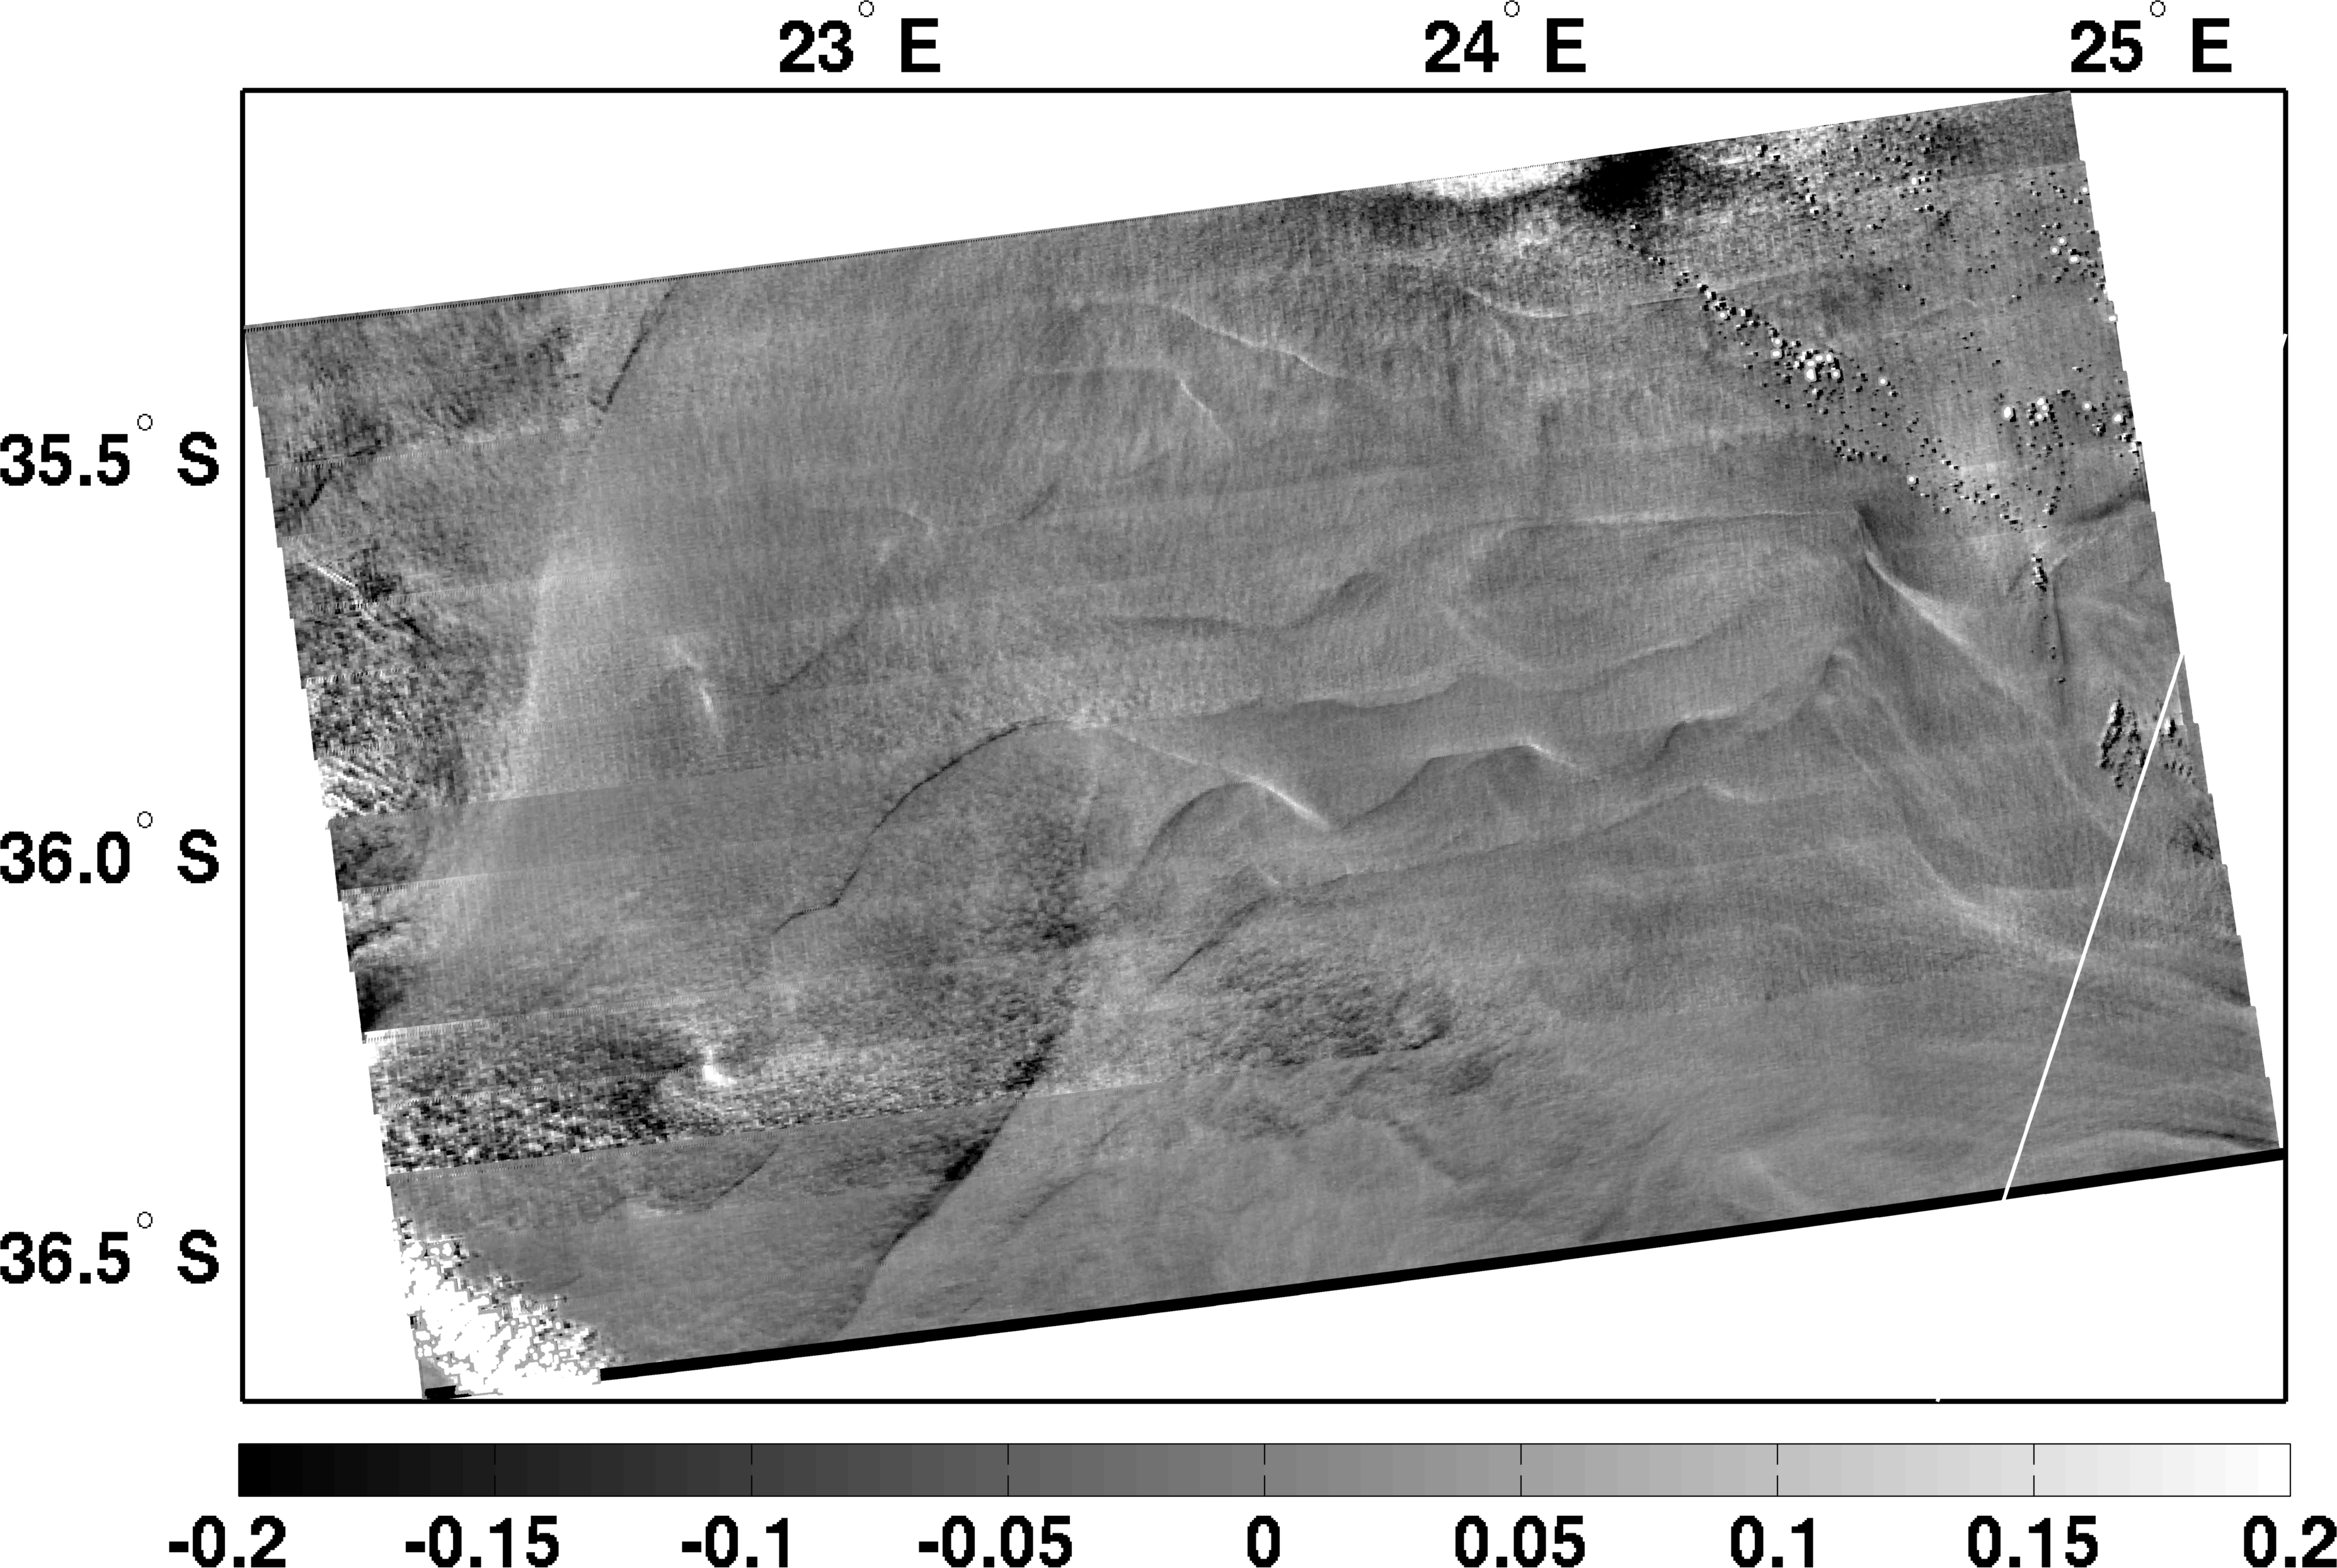
\includegraphics[width=1\linewidth]{fig3_8a}}
	\end{minipage}
	\hfill
	\begin{minipage}{.47\textwidth}
	    \subcaptionbox{\label{fig:3.8b}}
		{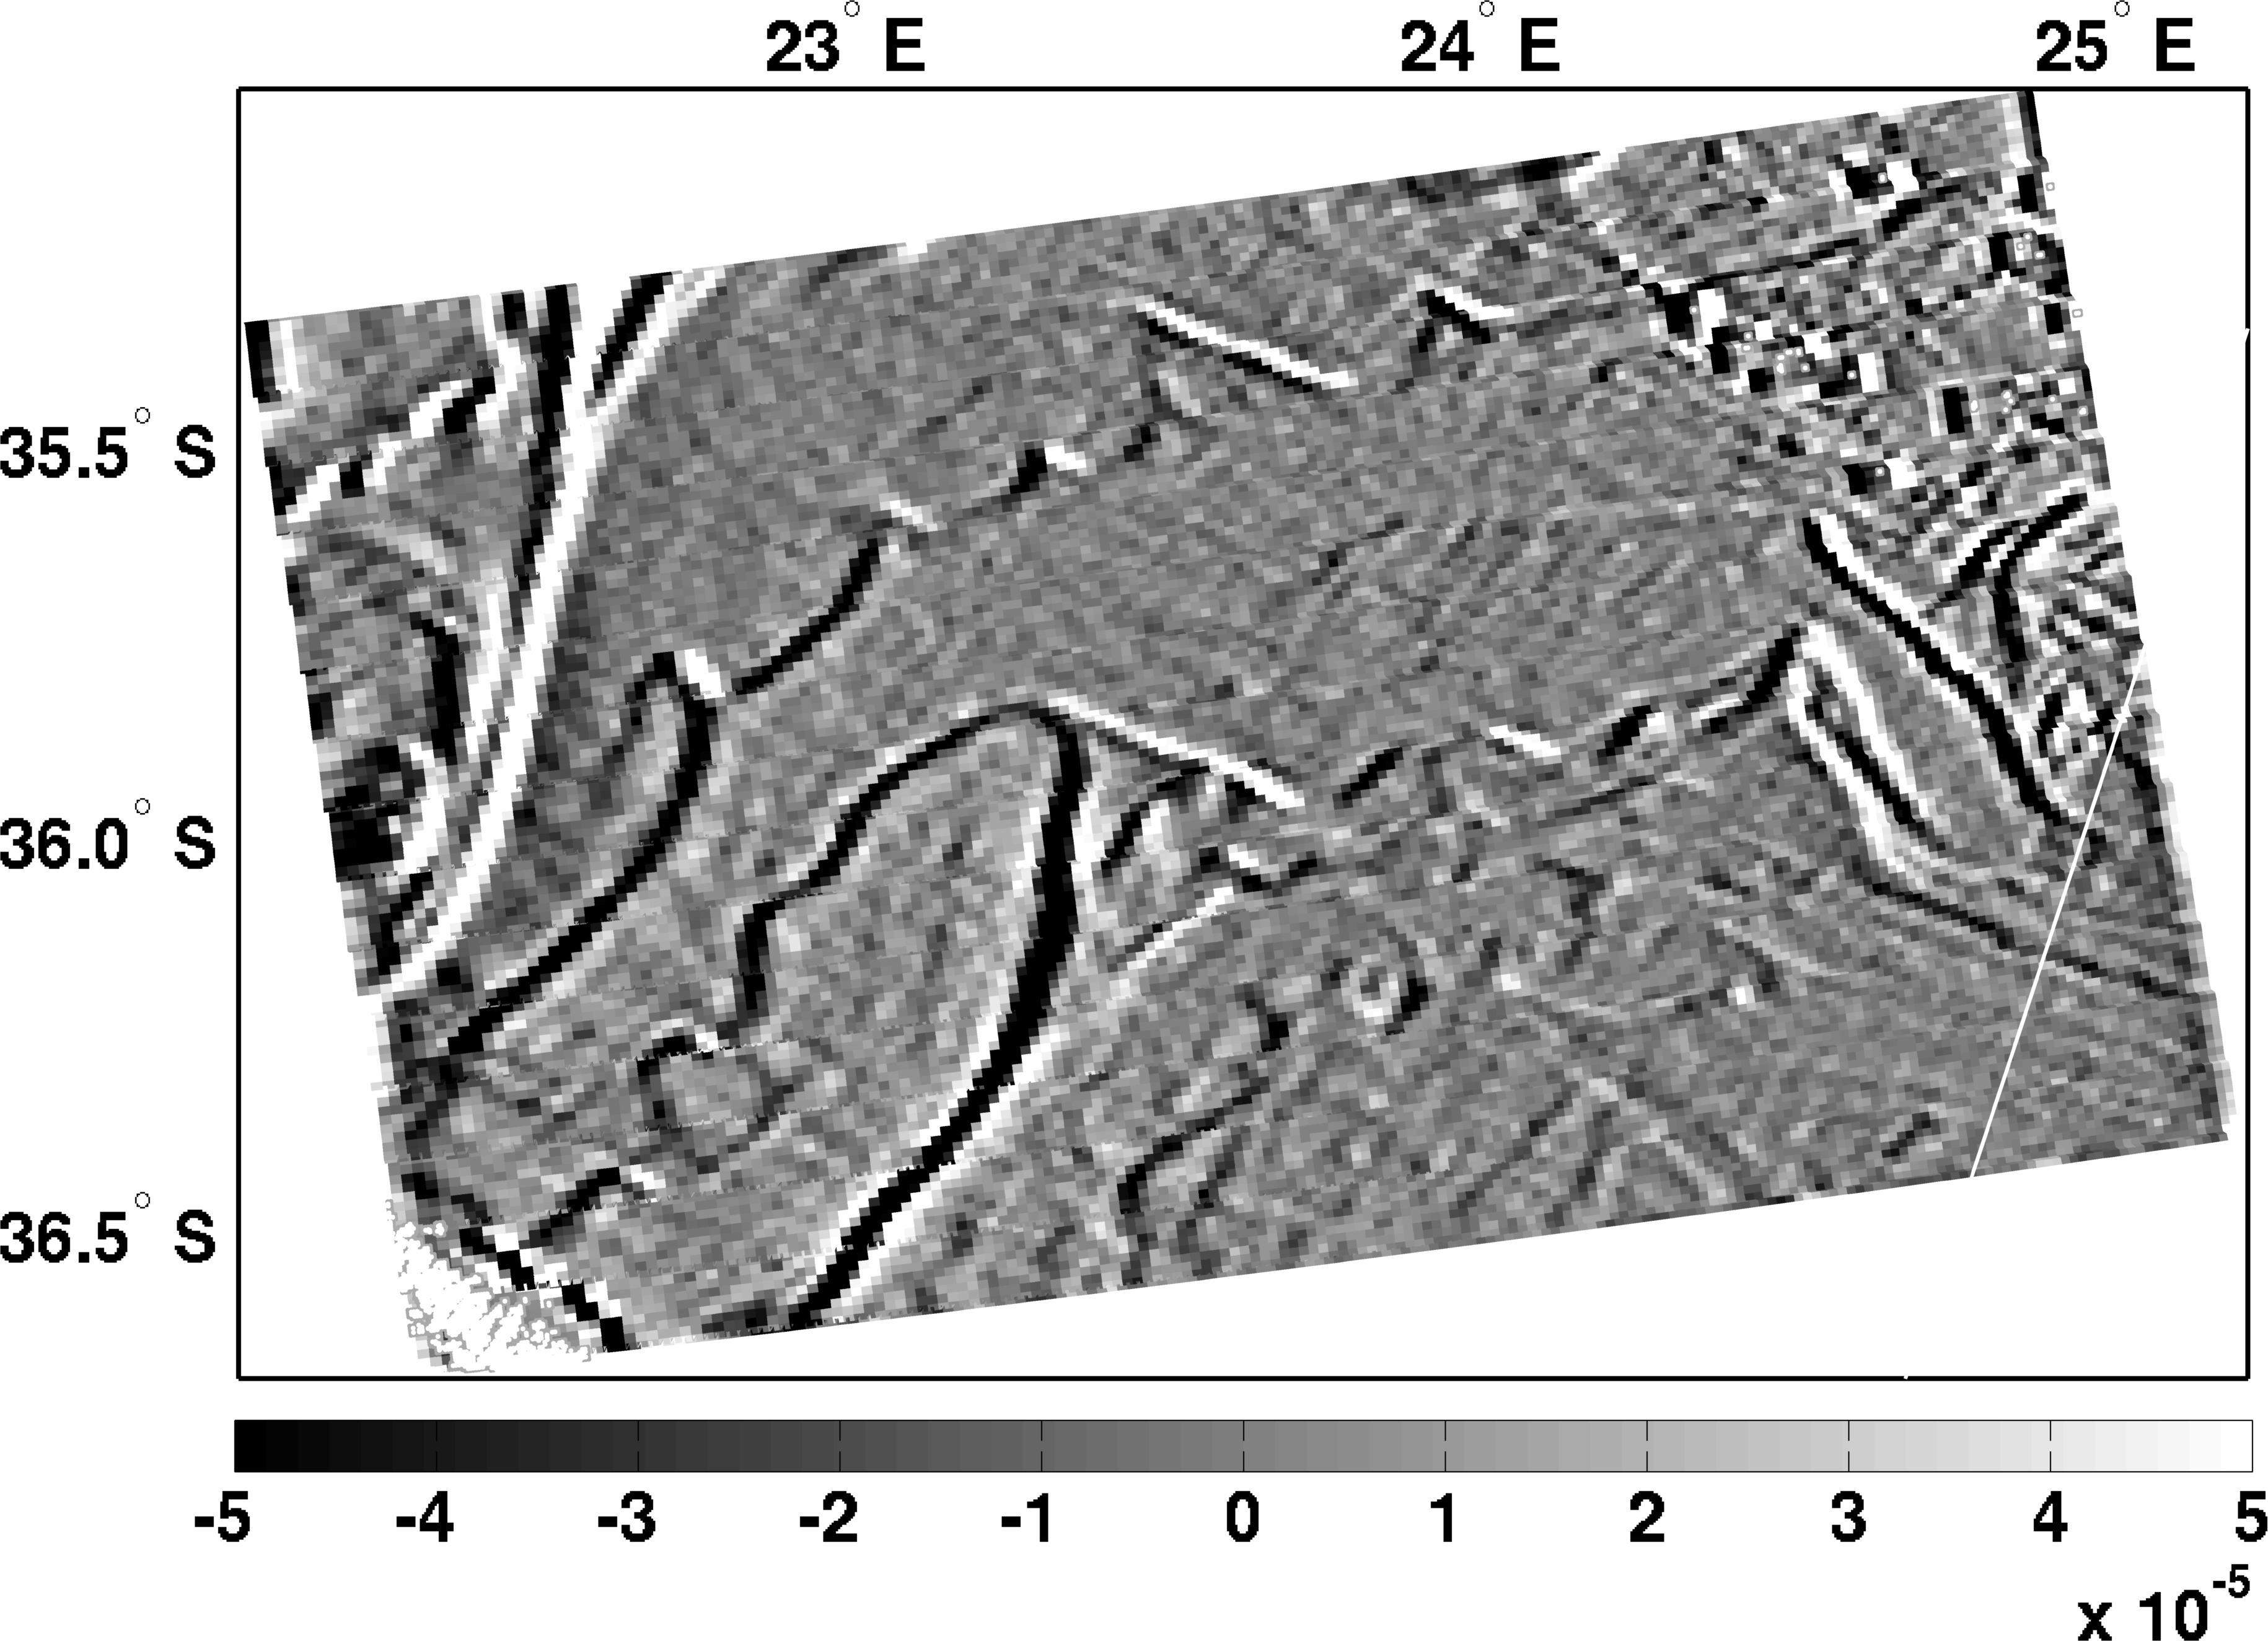
\includegraphics[width=1\linewidth]{fig3_8b}}
	\end{minipage}
    \\
    \floattitle{(а) Фрагмент поля контрастов СКН, показанный ранее на Рисунке~\ref{fig:3.5} (контур фрагмента выделен жёлтым цветом). (б) Поле дивергенции поверхностного течения. Наблюдаемое различие между полями дивергенции поверхностного течения на Рисунке~\ref{fig:3.8b} и соответствующей областью на Рисунке~\ref{fig:3.6b}, объясняется тем, что $\nabla \cdot {\it u}$, показанная на данном рисунке, рассчитывалась для локального Северного ветра, в то время как $\nabla \cdot {\it u}$, показанная на Рисунке~\ref{fig:3.6b} в этом же районе, была рассчитана для Южного ветра (подробнее в тексте). Яркие области на рисунке (б) соответствуют конвергенции течения, а тёмные -- дивергенции (детальнее см. подпись к Рисунку~\ref{fig:3.6})}
    \caption{Фрагменты поля контрастов СКН и дивергенции поверхностного течения}
    \label{fig:3.8}
\end{figure}


На Рисунке~\ref{fig:3.9}, в поле ТПО (Рисунок~\ref{fig:3.9a}), а также в поле дивергенции поверхностного течения (Рисунок~\ref{fig:3.9b}), отчётливо видна пара вихрей, образующих грибовидную структуру. Вместе с соответствующими полями СКН (Рисунок~\ref{fig:3.9c}) и контрастами УЭПР РСА (Рисунок~\ref{fig:3.9d}), изображающими ту же пару вихрей, рисунки отражают поражающие возможности синергетического метода. \textbf{Текстурное соответствие поверхностных проявлений в наблюдаемых полях ТПО, УЭПР, СКН и конвергенции, в частности для антициклонического вихря, лишь усиливает численный анализ динамики верхнего слоя океана.}\todo{???}



\begin{figure}[H]
   	\centering
	\begin{minipage}{.47\textwidth}
	    \subcaptionbox{\label{fig:3.9a}}
		{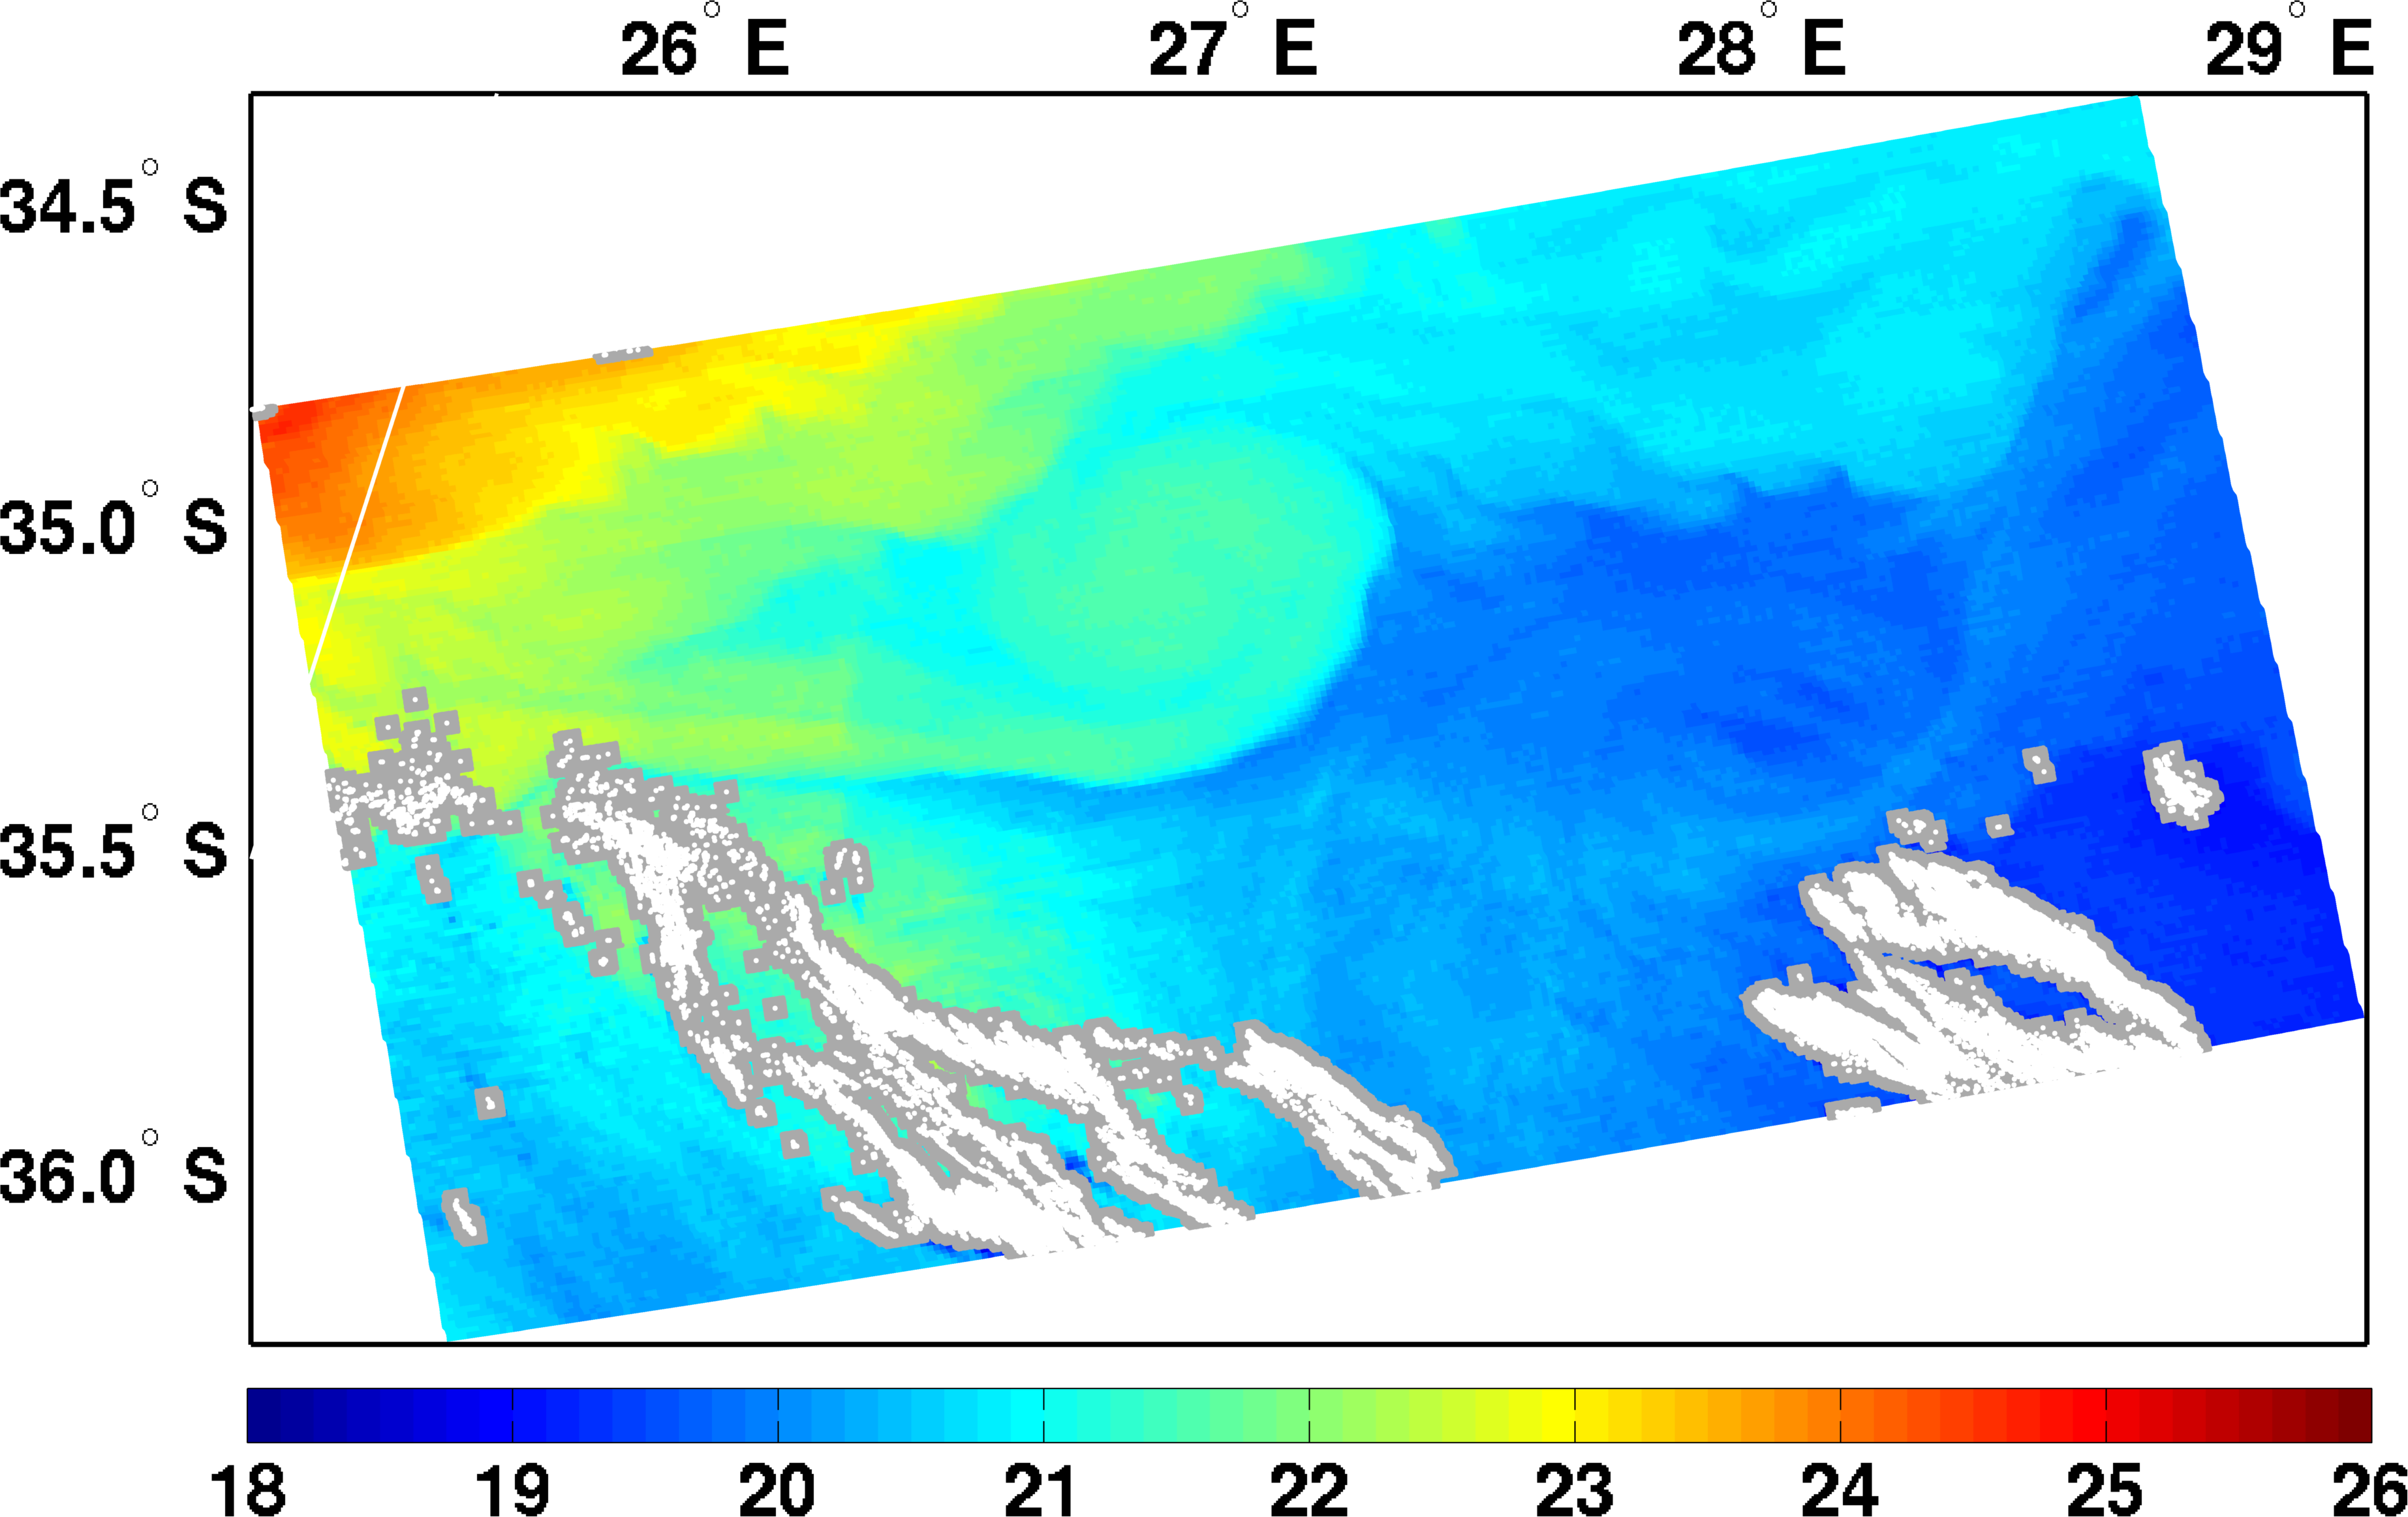
\includegraphics[width=1\linewidth]{fig3_9a}}
	\end{minipage}
	\hfill
	\begin{minipage}{.47\textwidth}
	    \subcaptionbox{\label{fig:3.9b}}
		{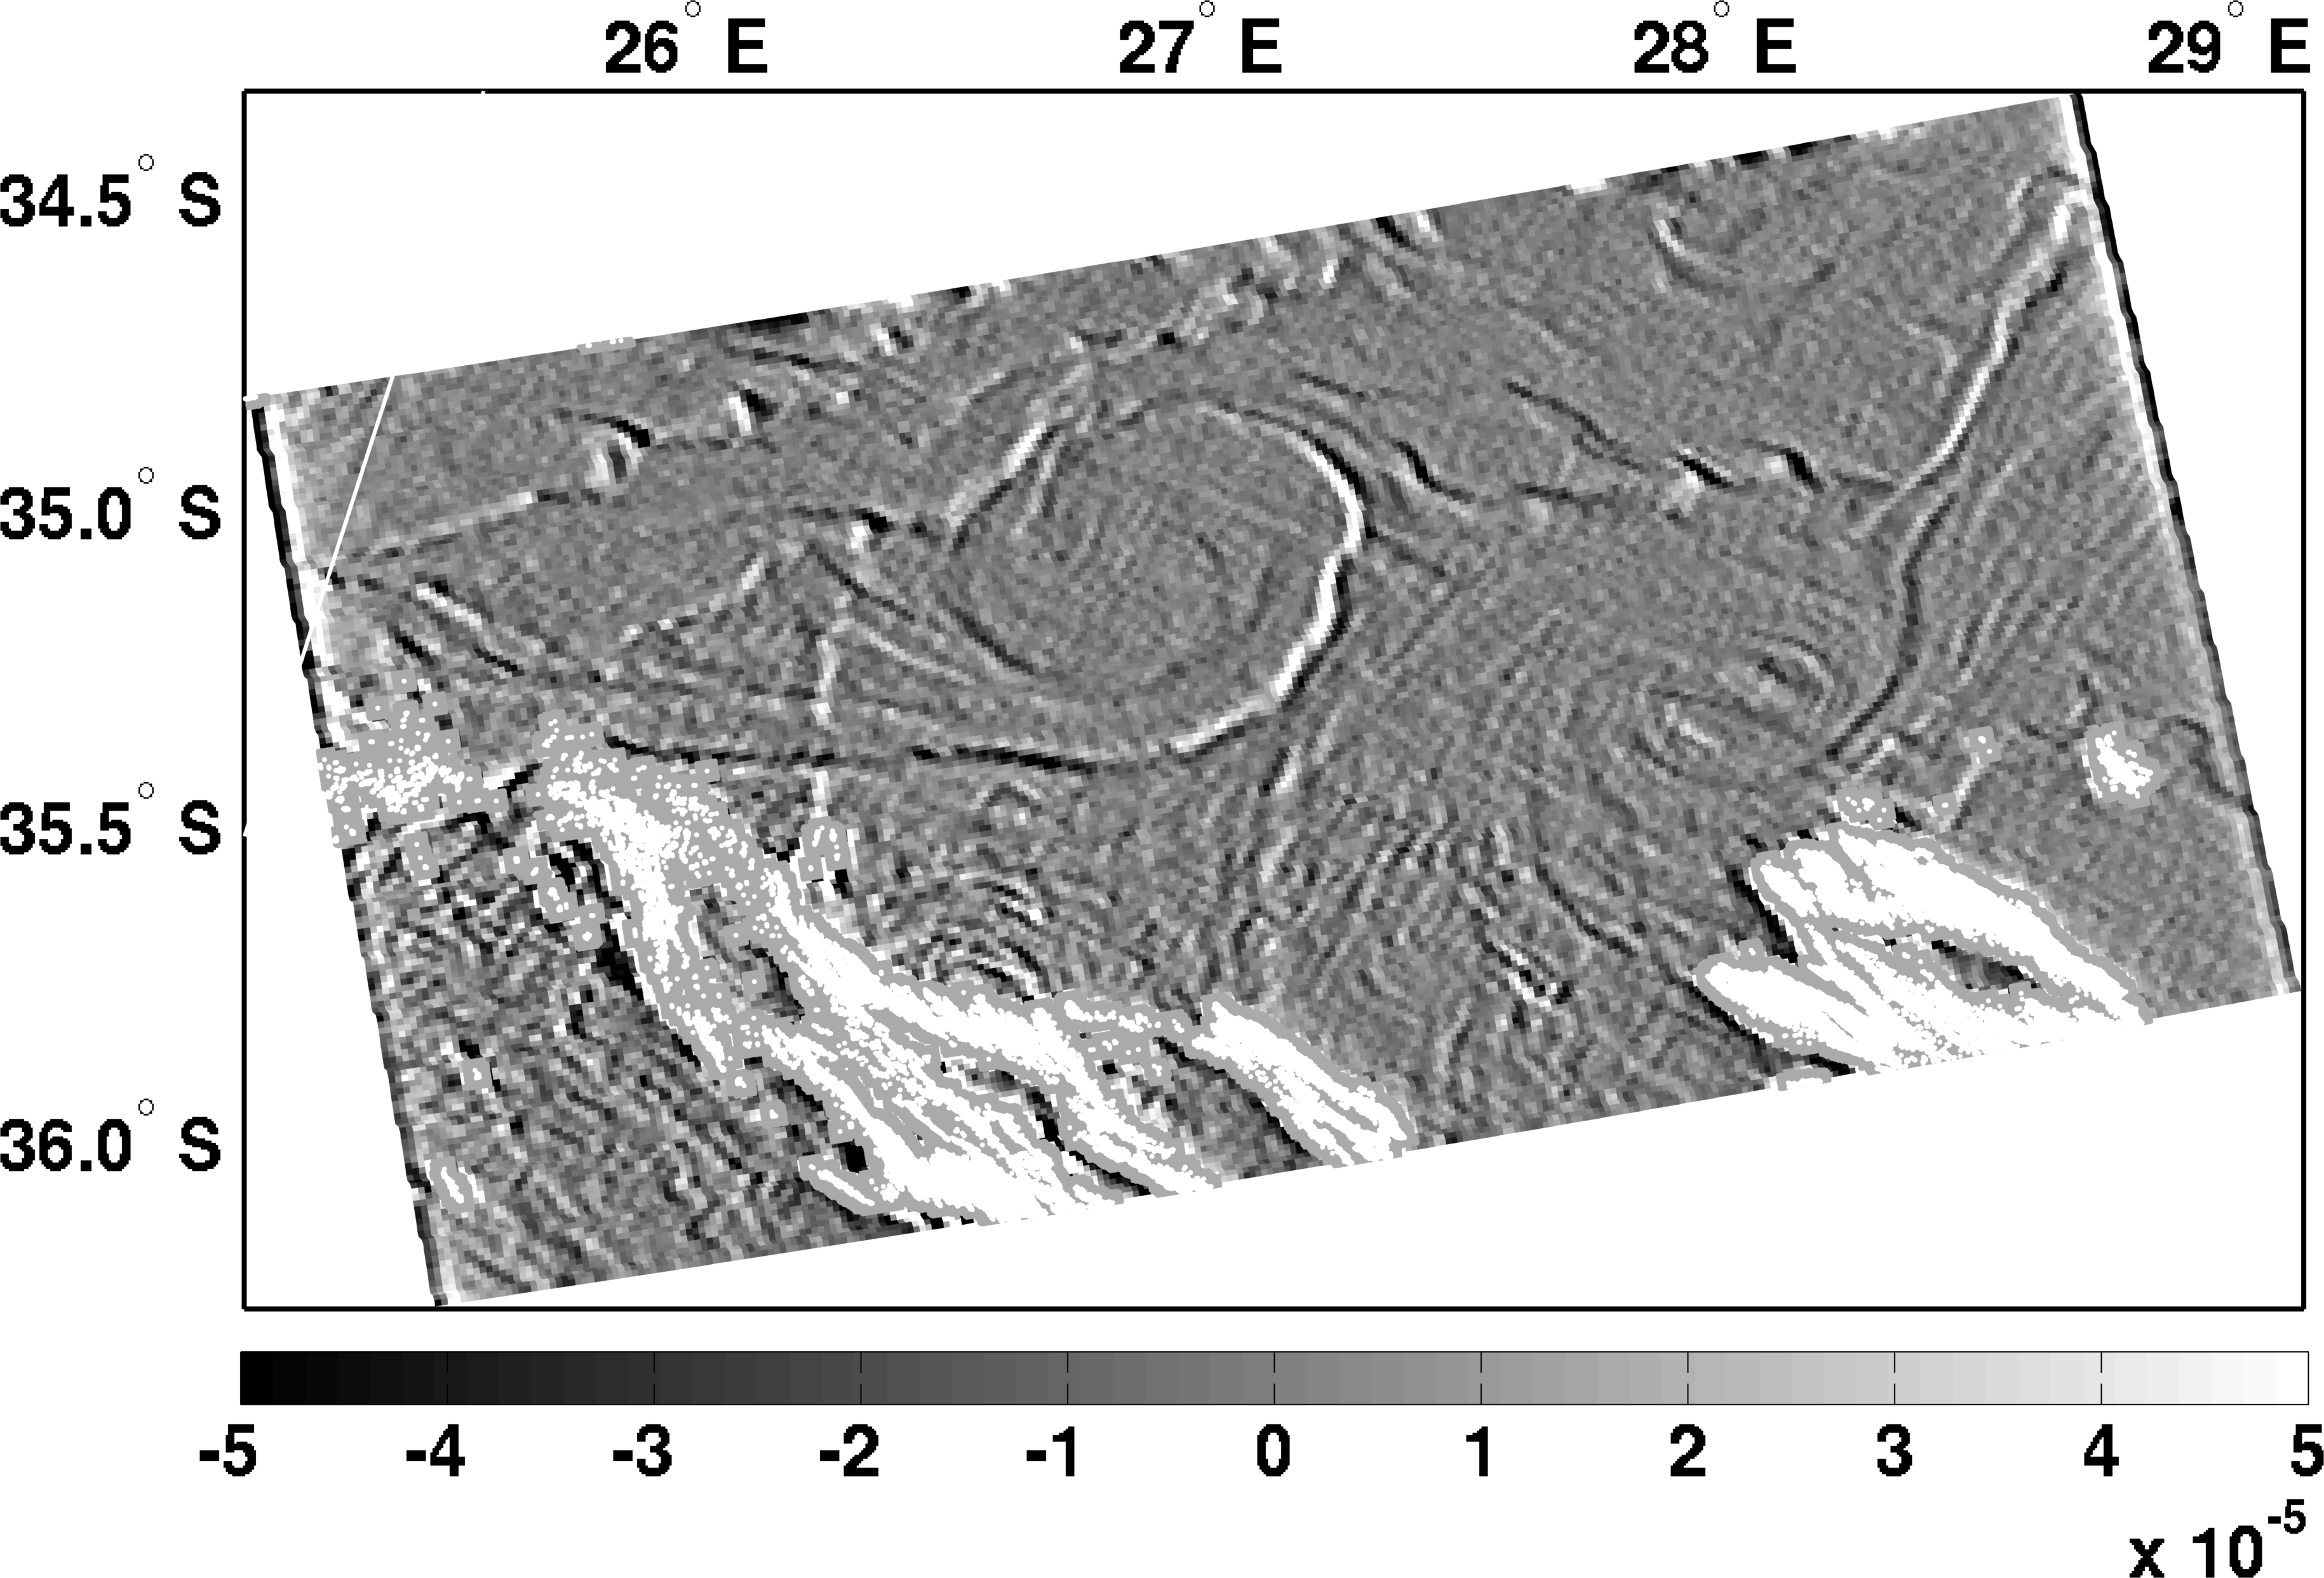
\includegraphics[width=1\linewidth]{fig3_9b}}
	\end{minipage}
	\\
	\begin{minipage}{.47\textwidth}
	    \subcaptionbox{\label{fig:3.9c}}
		{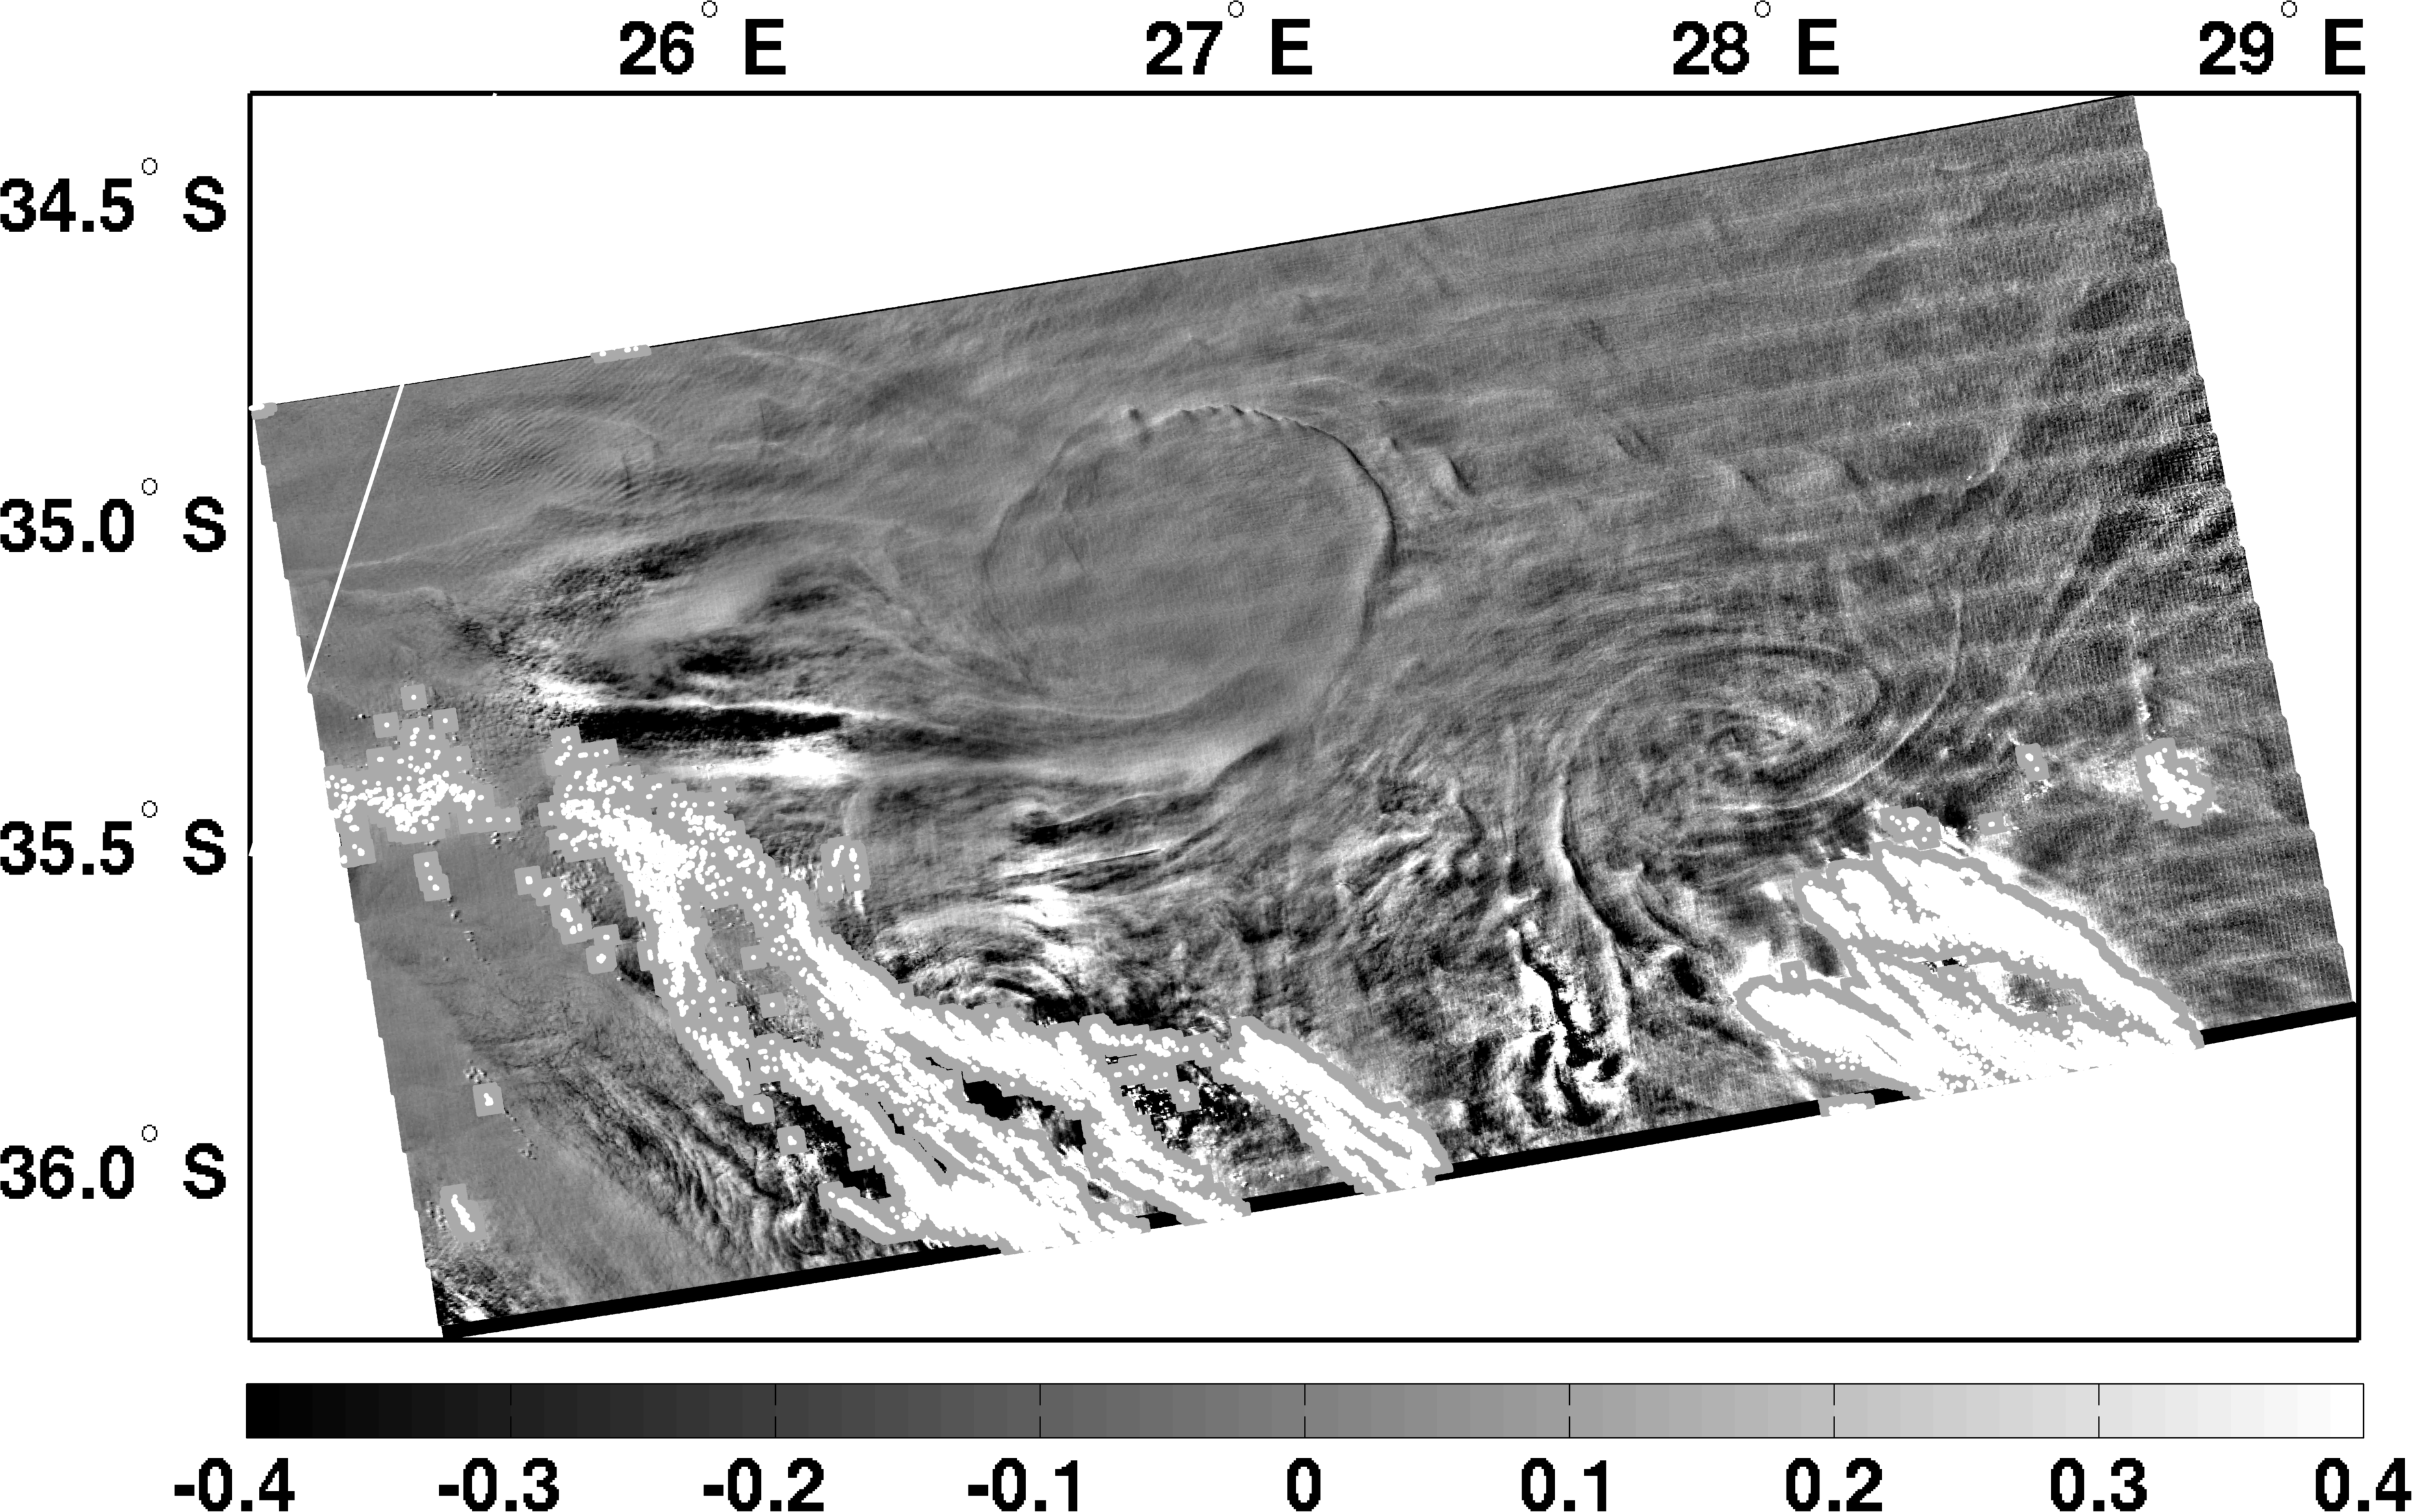
\includegraphics[width=1\linewidth]{fig3_9c}}
	\end{minipage}
	\hfill
	\begin{minipage}{.47\textwidth}
	    \subcaptionbox{\label{fig:3.9d}}
		{\includegraphics[width=1\linewidth]{fig3_9d}}
	\end{minipage}
    \\
    \floattitle{Поле ТПО MODIS (а), а также в поле дивергенции поверхностного течения (б), отчётливо видна пара вихрей диаметром 120км, образующих грибовидную структуру. Соответствующие поля СКН (в) и контрасты УЭПР РСА в линейных единицах (г), изображают ту же пару вихрей. Рисунки отражают поражающие возможности синергетического метода. Яркие области на рисунке (б) соответствуют конвергенции течения, а тёмные -- дивергенции (детальнее см. подпись к Рисунку~\ref{fig:3.6b})}
    \caption{Фрагменты поля контрастов СКН и дивергенции поверхностного течения}
    \label{fig:3.9}
\end{figure}



\section{Интерпретация данных наблюдений на основе модельных представлений} \label{sec:3.3}


Поле поверхностного течения (состоящее из суммы КГТ, Экмановского дрифта и ВАЦ), полученное по данным ТПО MODIS и полям ветра ENVISAT ASAR, используется в качестве входных параметров модели формирования РЛ-изображения RIM (от англ. Radar Imaging Model), для симулирования РСА УЭПР и СКН сигнатур, как изложено в \citep{Kudryavtsev2005,Johannessen2005}. RIM моделирует проявления особенностей поверхностного течения, температурных фронтов и сликов в терминах модуляции ветро-волнового спектра, СКН, обрушения ветровых волн и УЭПР. 

Поле скорости поверхностного (именно КГТ по полю темпнратуры) течения восстановленного по \dots \dots .. приведено на рис\dots \dots 

Функция тока

Завихренность и Дивергенция



\begin{figure}[H]
    
\includegraphics[width=\linewidth]{fig3_10}
    \floattitle{(слева) Сечение через контрасты спектра брэгговских волновых чисел, нормированных на фоновый спектр, рассчитанные по модели RIM для бокового ветра (сплошная синяя линия) и направления визирования против ветра (красная линия с крестиками). (справа) Контрасты спектра брэгговских волновых чисел для различных направлений ветра. Отчётливо видно, что для бокового ветра вариации контрастов значительно выше, а для направлений против и по ветру -- они минимальны}
    \caption{Различия контрастов спектра брэгговских волновых чисел, рассчитанных для случая, приведённого на Рисунке~35, при различных направлениях ветра для случайного сечения}
    \label{fig:3.10}
\end{figure}



\subsection{Результаты интерпретации данных} \label{sec:3.3.1}


Поле течений представленное на рисунке (КГТ, Функция тока и т.д) использовались как входные параметры для расчёта трансформации эволюции спектров волн, а также СКН по модели RIM. Основные соотношения модели приведены в \todo{Приложении}. Смоделированные поверхностные проявления грибовидного вихря в терминах СКН, обрушений волн и контрастов УЭПР приводятся на Рисунке~35 для угла падения 30${}^\circ$ и угла между вектором скорости ветра и направлением дальности 20${}^\circ$. Как и ожидалось, паттерны этих двумерных полей очень схожи со структурой поля конвергенции поверхностного течения. Если присмотреться, можно заметить, что увеличение контрастов всех трёх характеристик происходит в области конвергенции течения (яркие области в верхнем левом углу изображения), в то время, как подавление возникает в зонах дивергенции (тёмные области). Этот результат численного моделирования соответствует упрощённому решению, определяемому уравнениями \eqref{eq:1.5}, \eqref{eq:1.7}, \eqref{eq:1.8} и \eqref{eq:1.9}. Стоит напомнить, что проявления особенностей мезомасштабных течений в УЭПР возникает в результате обрушений волн, обеспечивающих усиление/ослабление механических возмущений на поверхности в областях конвергенции/дивергенции. Это приводит к усилению/подавлению волн Брэгга и, тем самым, модуляции обратного рассеяния РЛ-сигнала. Сравнивая симулированные поля контрастов УЭПР и СКН с наблюдаемыми на Рисунке~33, можно заметить, что магнитуды модельных контрастов согласуются с наблюдаемыми значениями. Поскольку RIM была тщательно протестирована на имеющихся данных (см. \citep{Kudryavtsev2005}), этот факт предполагает, что восстановленные поля дивергенции поверхностного течения могут рассматриваться как близкие к ``реальным''. Также стоит отметить, что моделирование контрастов УЭПР для той же пары вихрей, без учёта влияния обрушений волн на УЭПР и модуляцию Брэгговских волн (``стандартная'' релаксационная модель) даёт контрасты УЭПР по величине на 4 порядка меньше, нежели приведённые на Рисунке~35.

Примеры результата расчётов СКН и обрушений волн с использованием уравнений \eqref{ZEqnNum135284} и \eqref{ZEqnNum272976} по модели RIM приводятся на Рисунке~35.

\begin{figure}[H]
   	\centering
	\begin{minipage}{.47\textwidth}
	    \subcaptionbox{\label{fig:3.11a}}
		{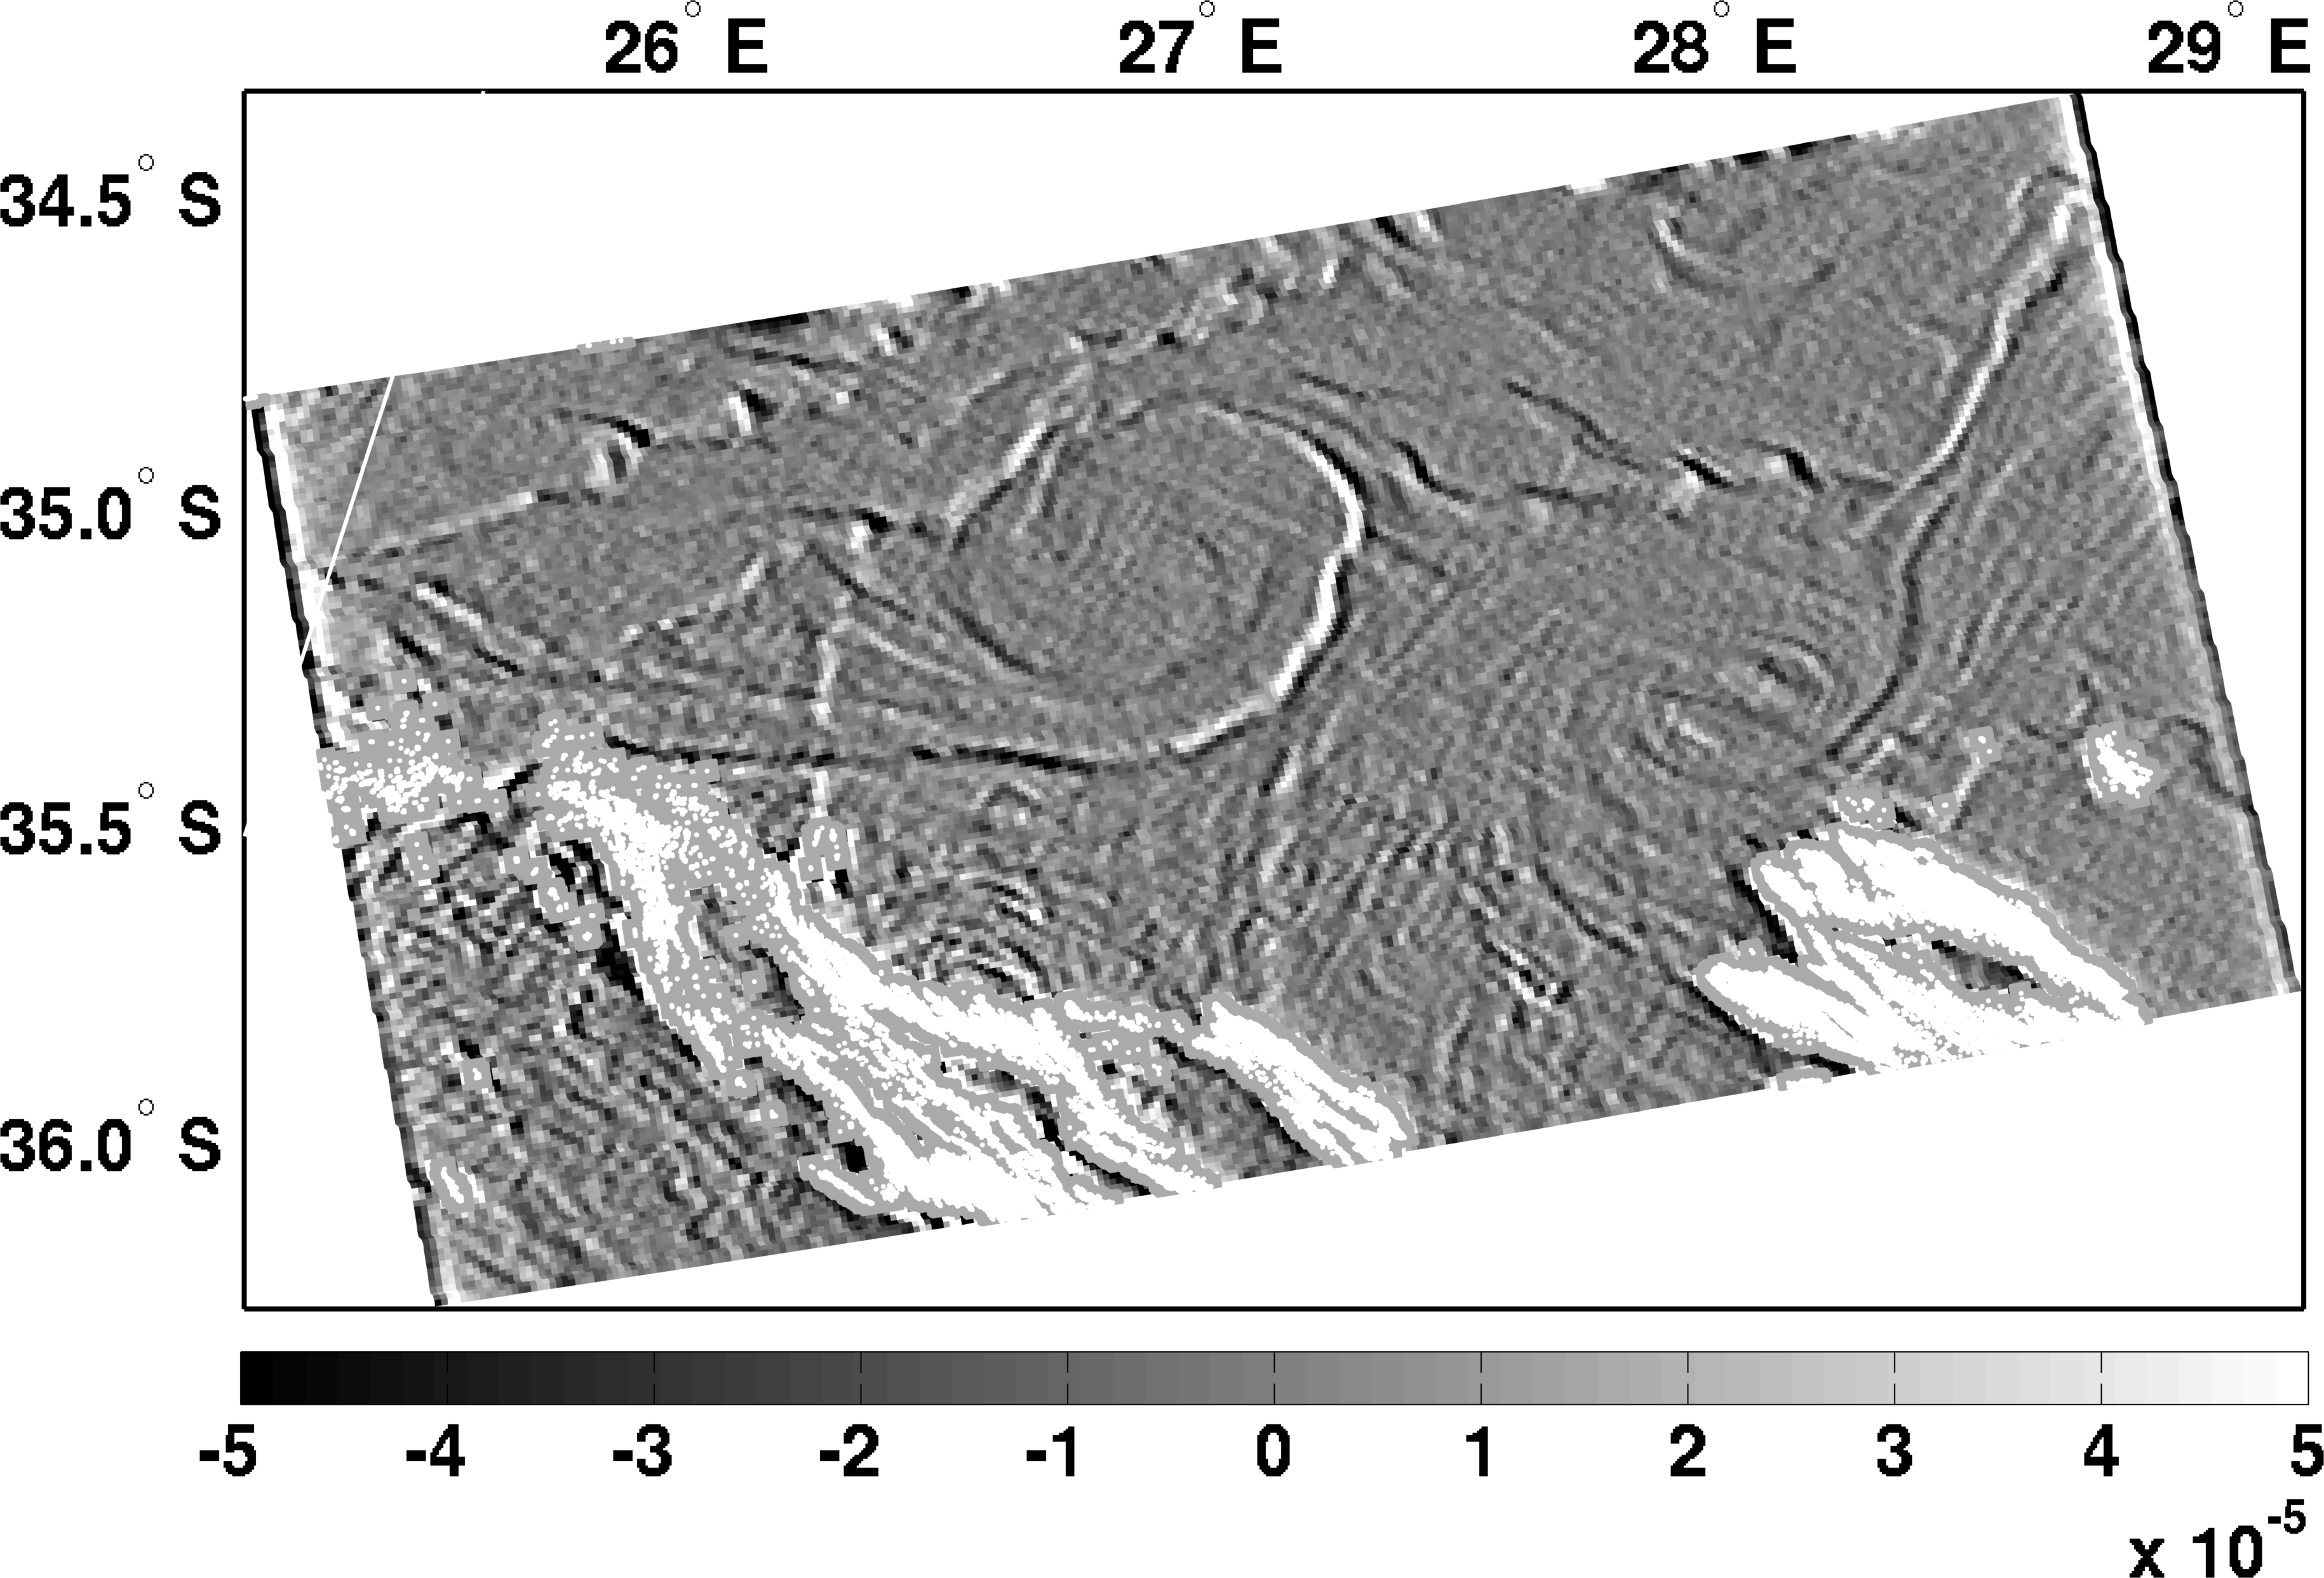
\includegraphics[width=1\linewidth]{fig3_11a}}
	\end{minipage}
	\hfill
	\begin{minipage}{.47\textwidth}
	    \subcaptionbox{\label{fig:3.11b}}
		{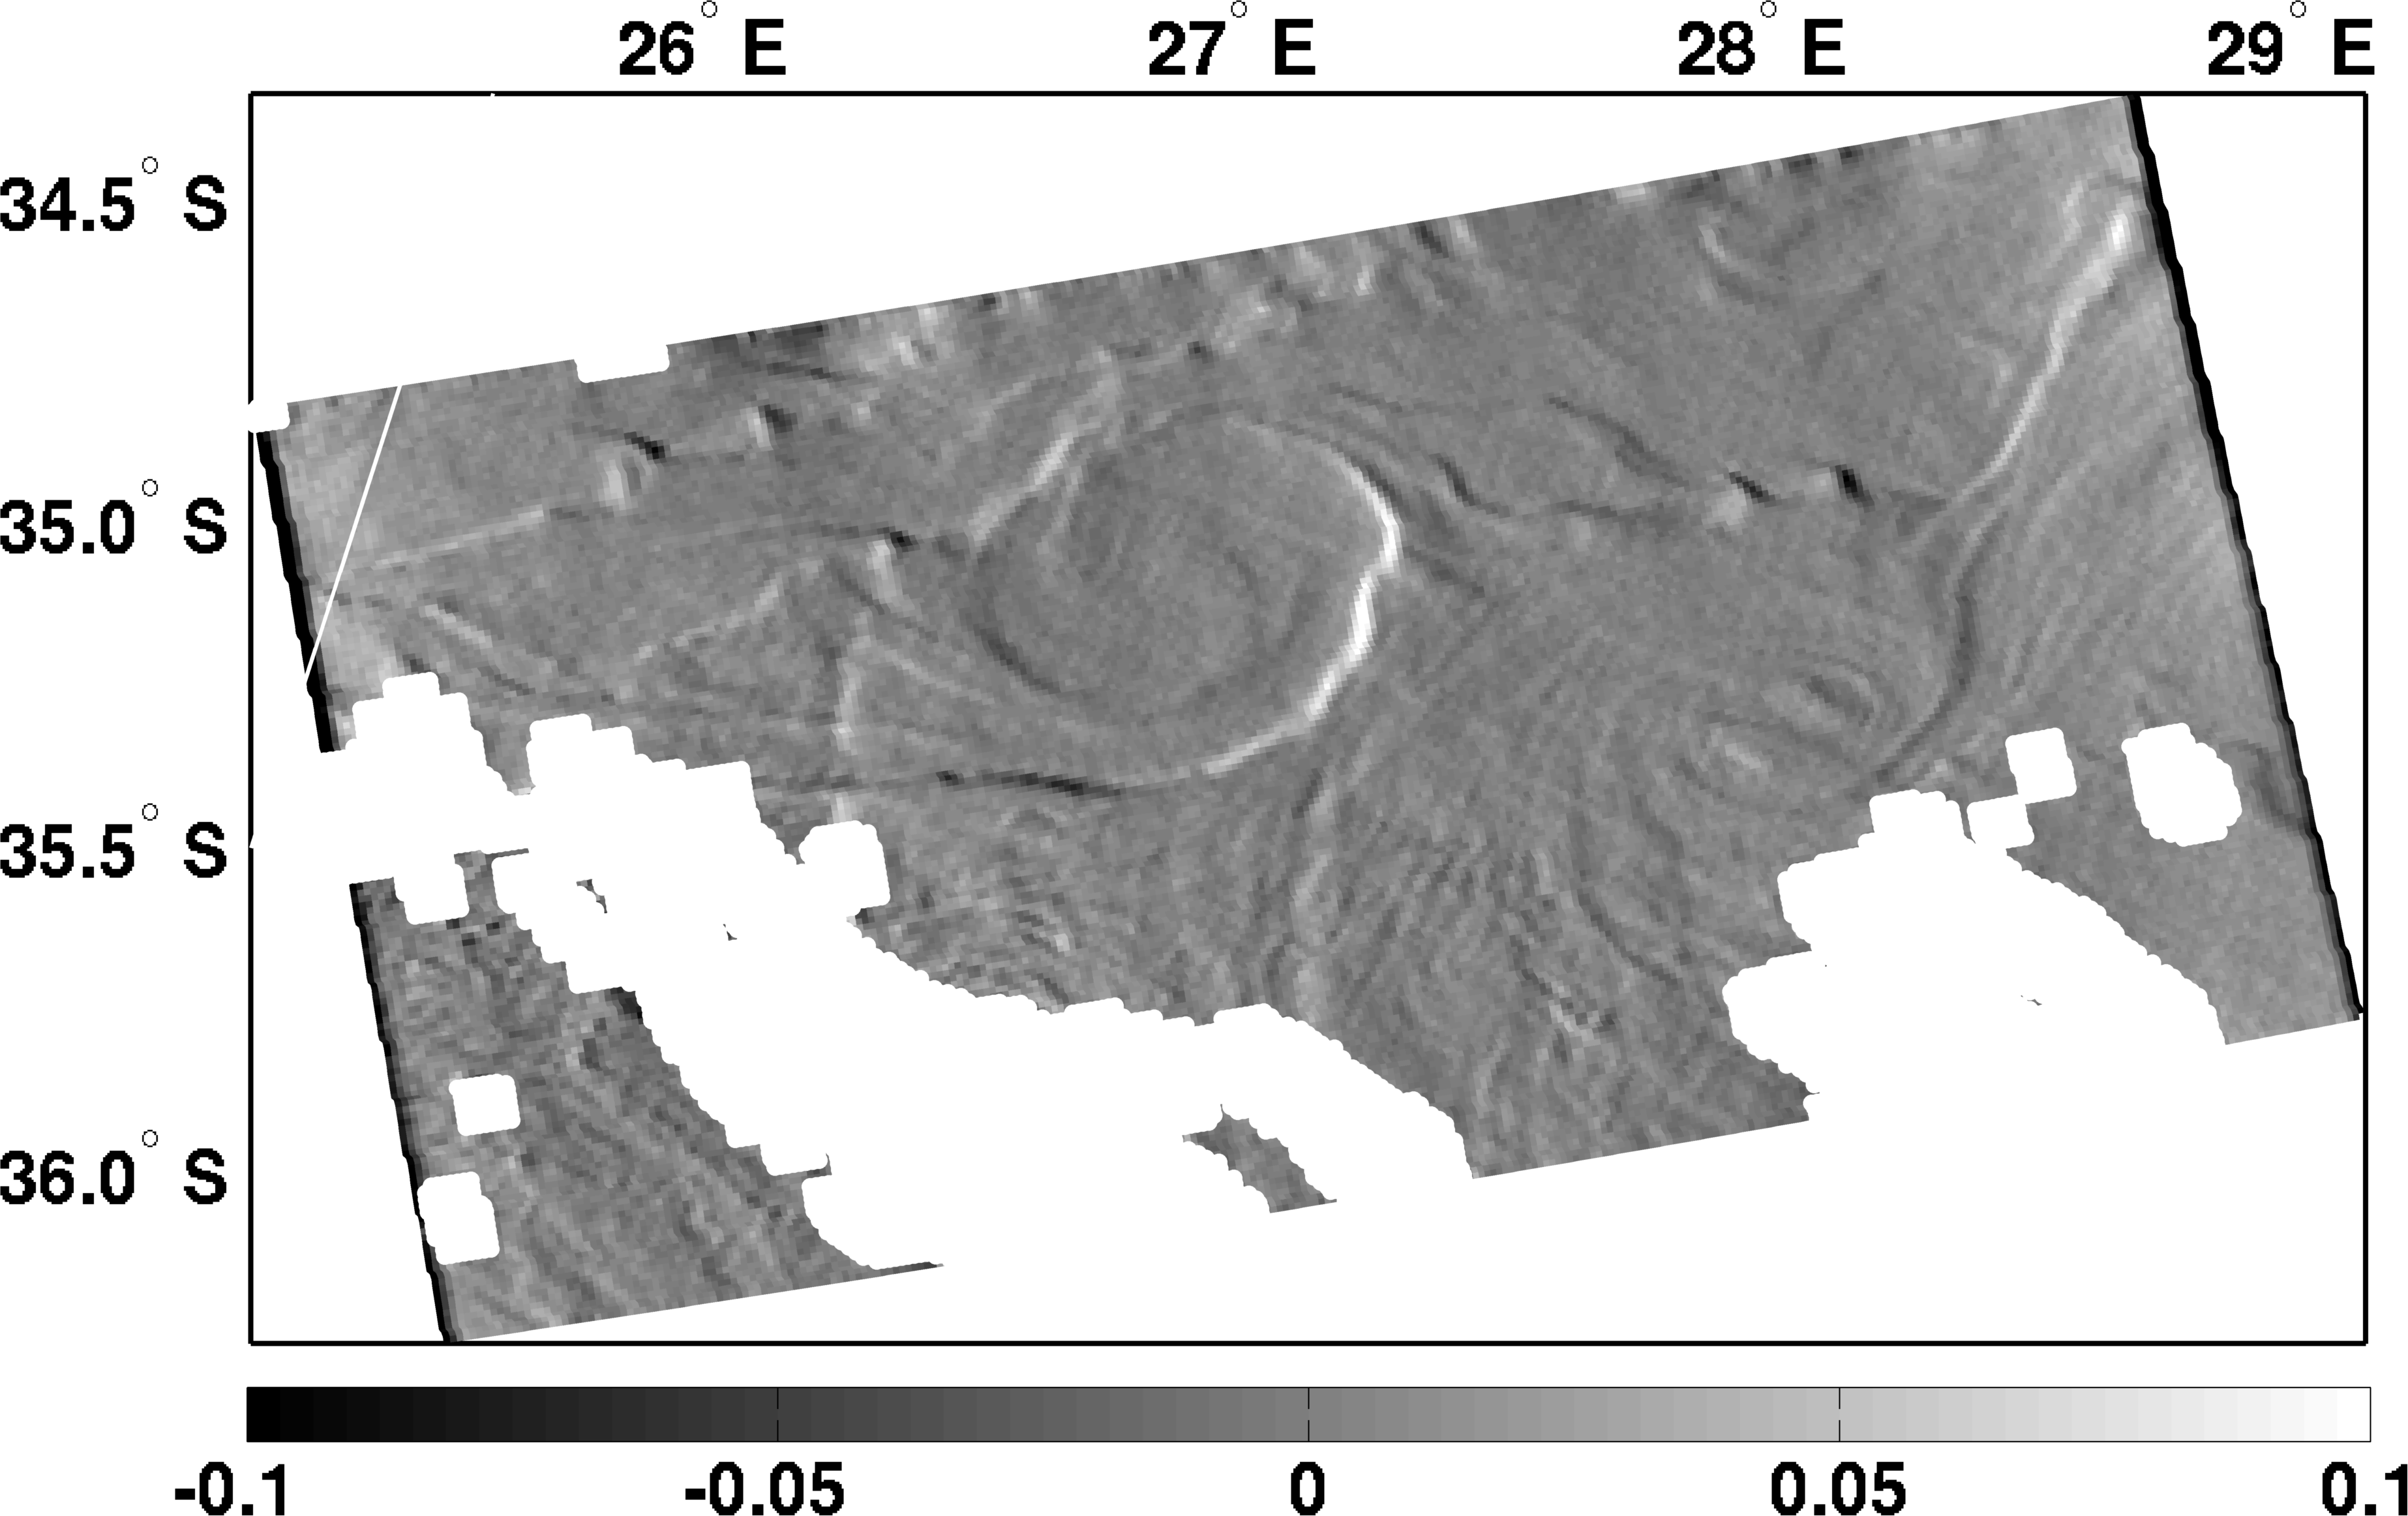
\includegraphics[width=1\linewidth]{fig3_11b}}
	\end{minipage}
	\\
	\begin{minipage}{.47\textwidth}
	    \subcaptionbox{\label{fig:3.11c}}
		{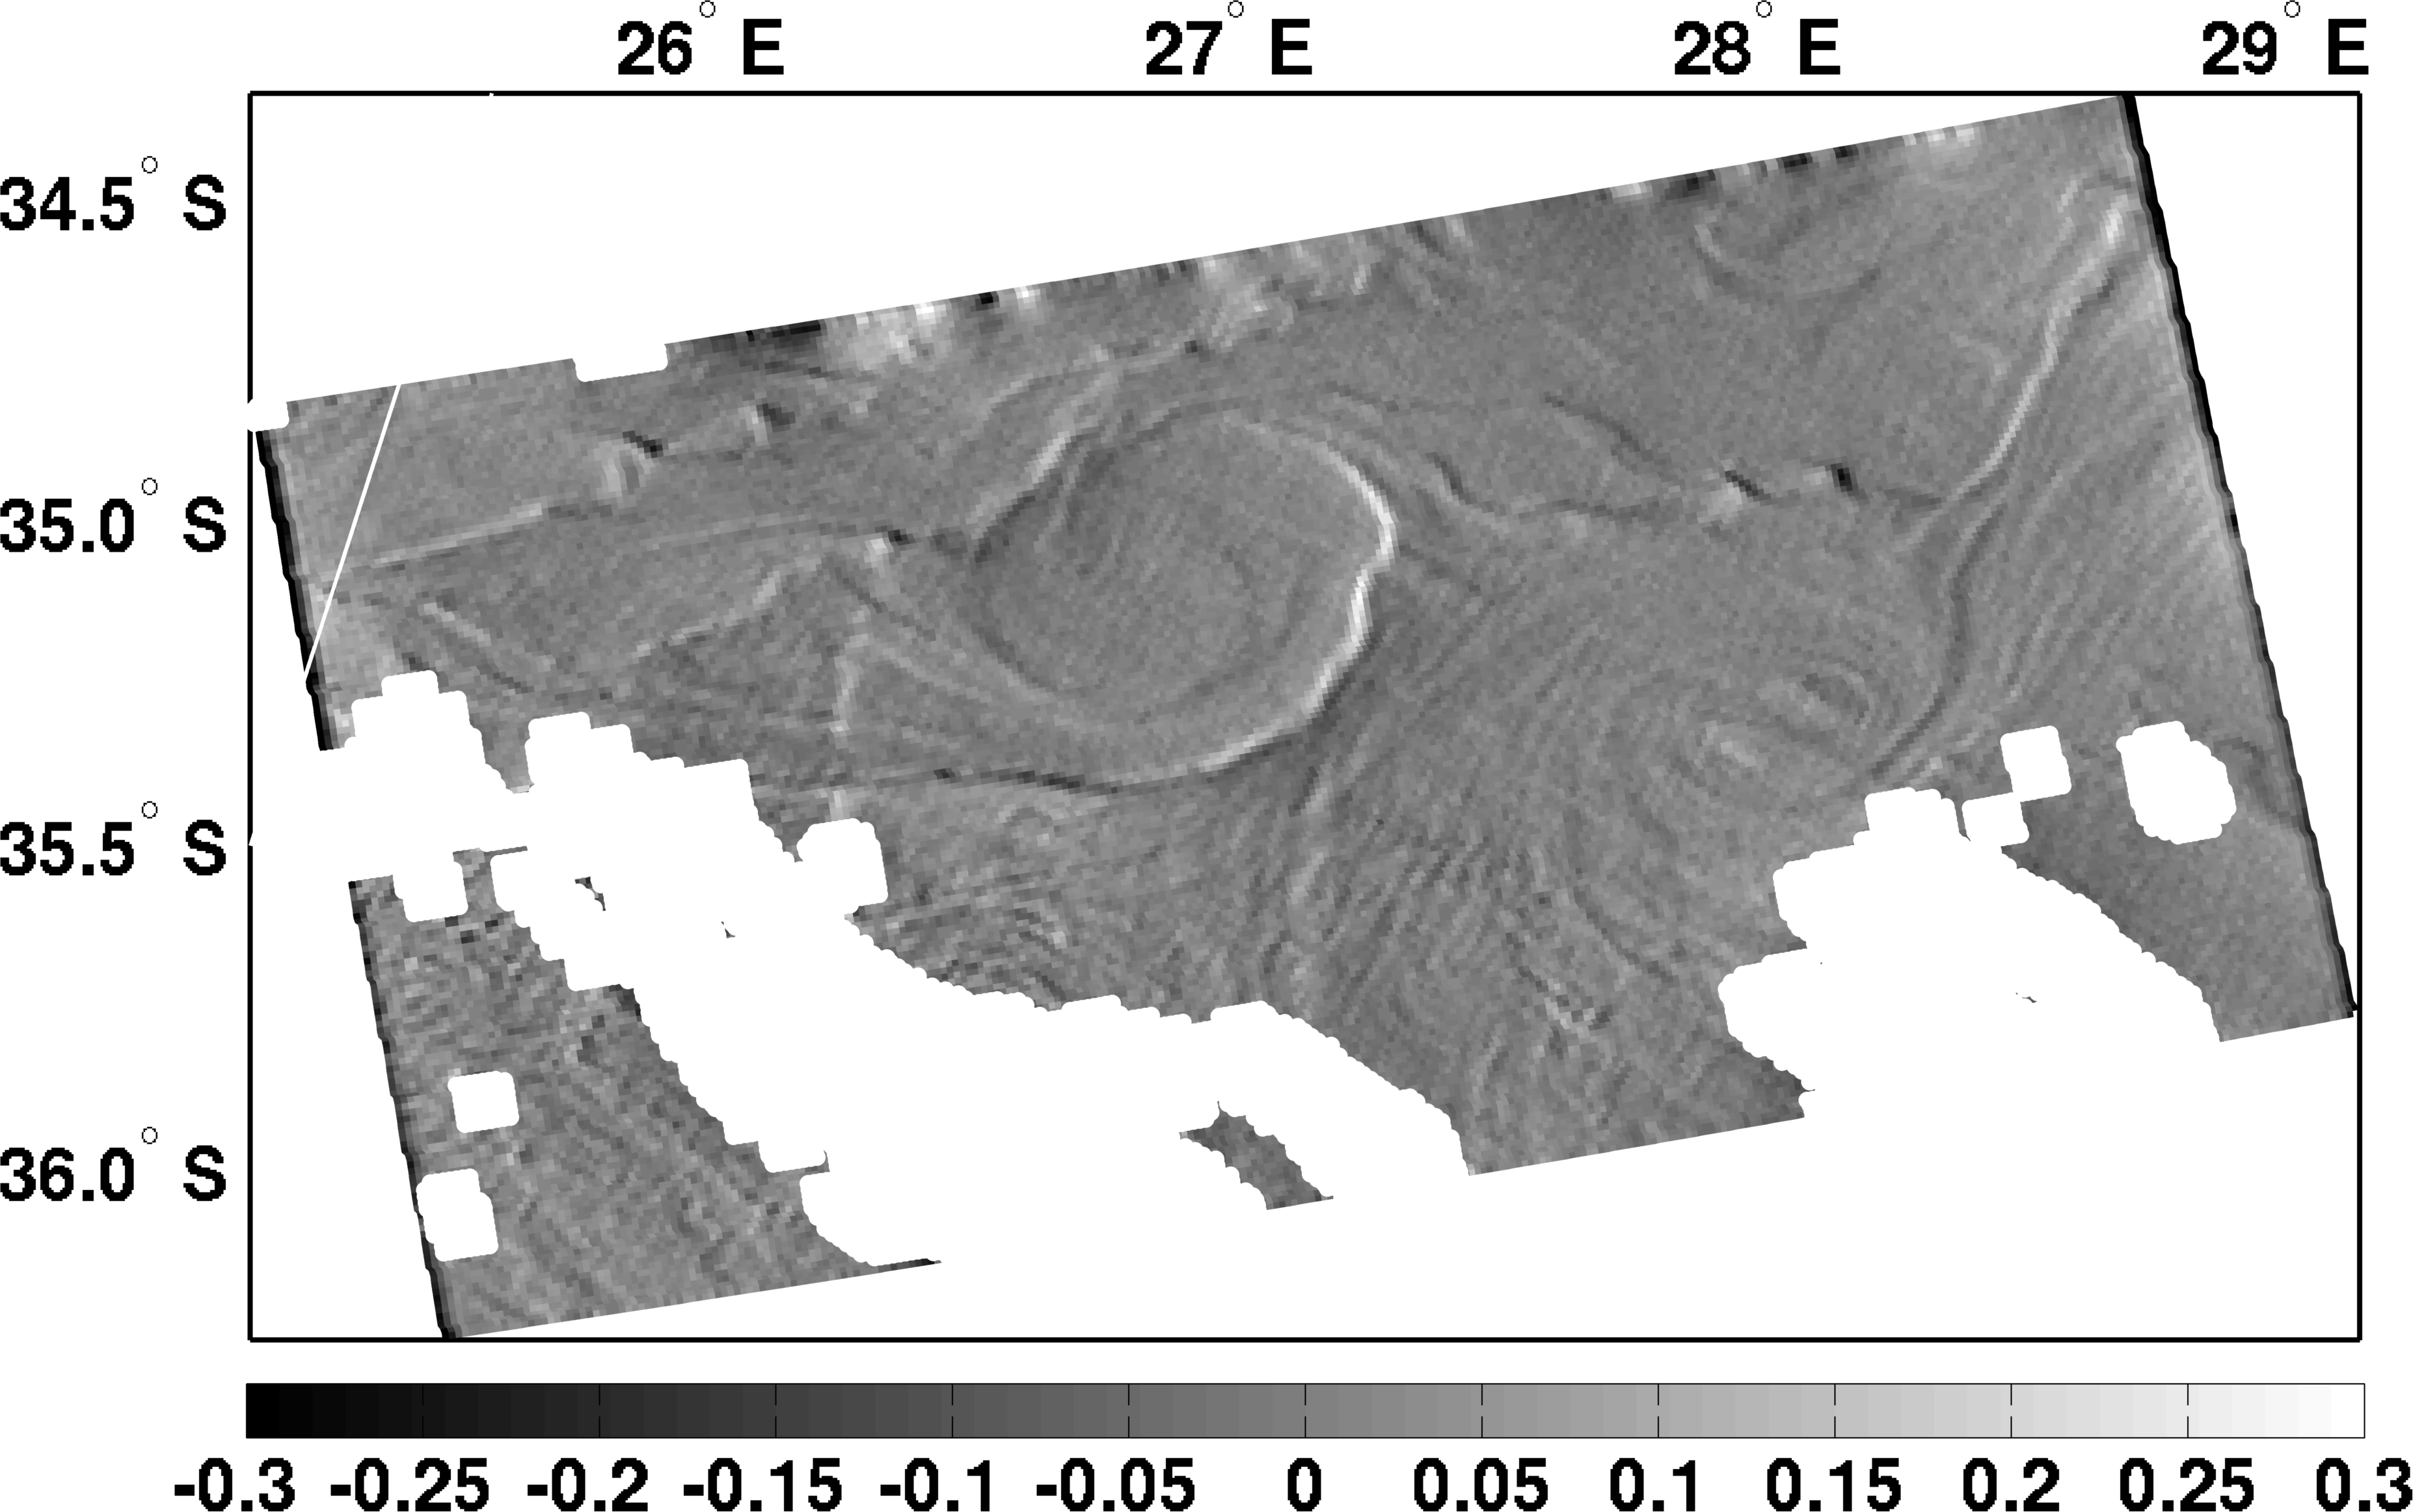
\includegraphics[width=1\linewidth]{fig3_11c}}
	\end{minipage}
	\hfill
	\begin{minipage}{.47\textwidth}
	    \subcaptionbox{\label{fig:3.11d}}
		{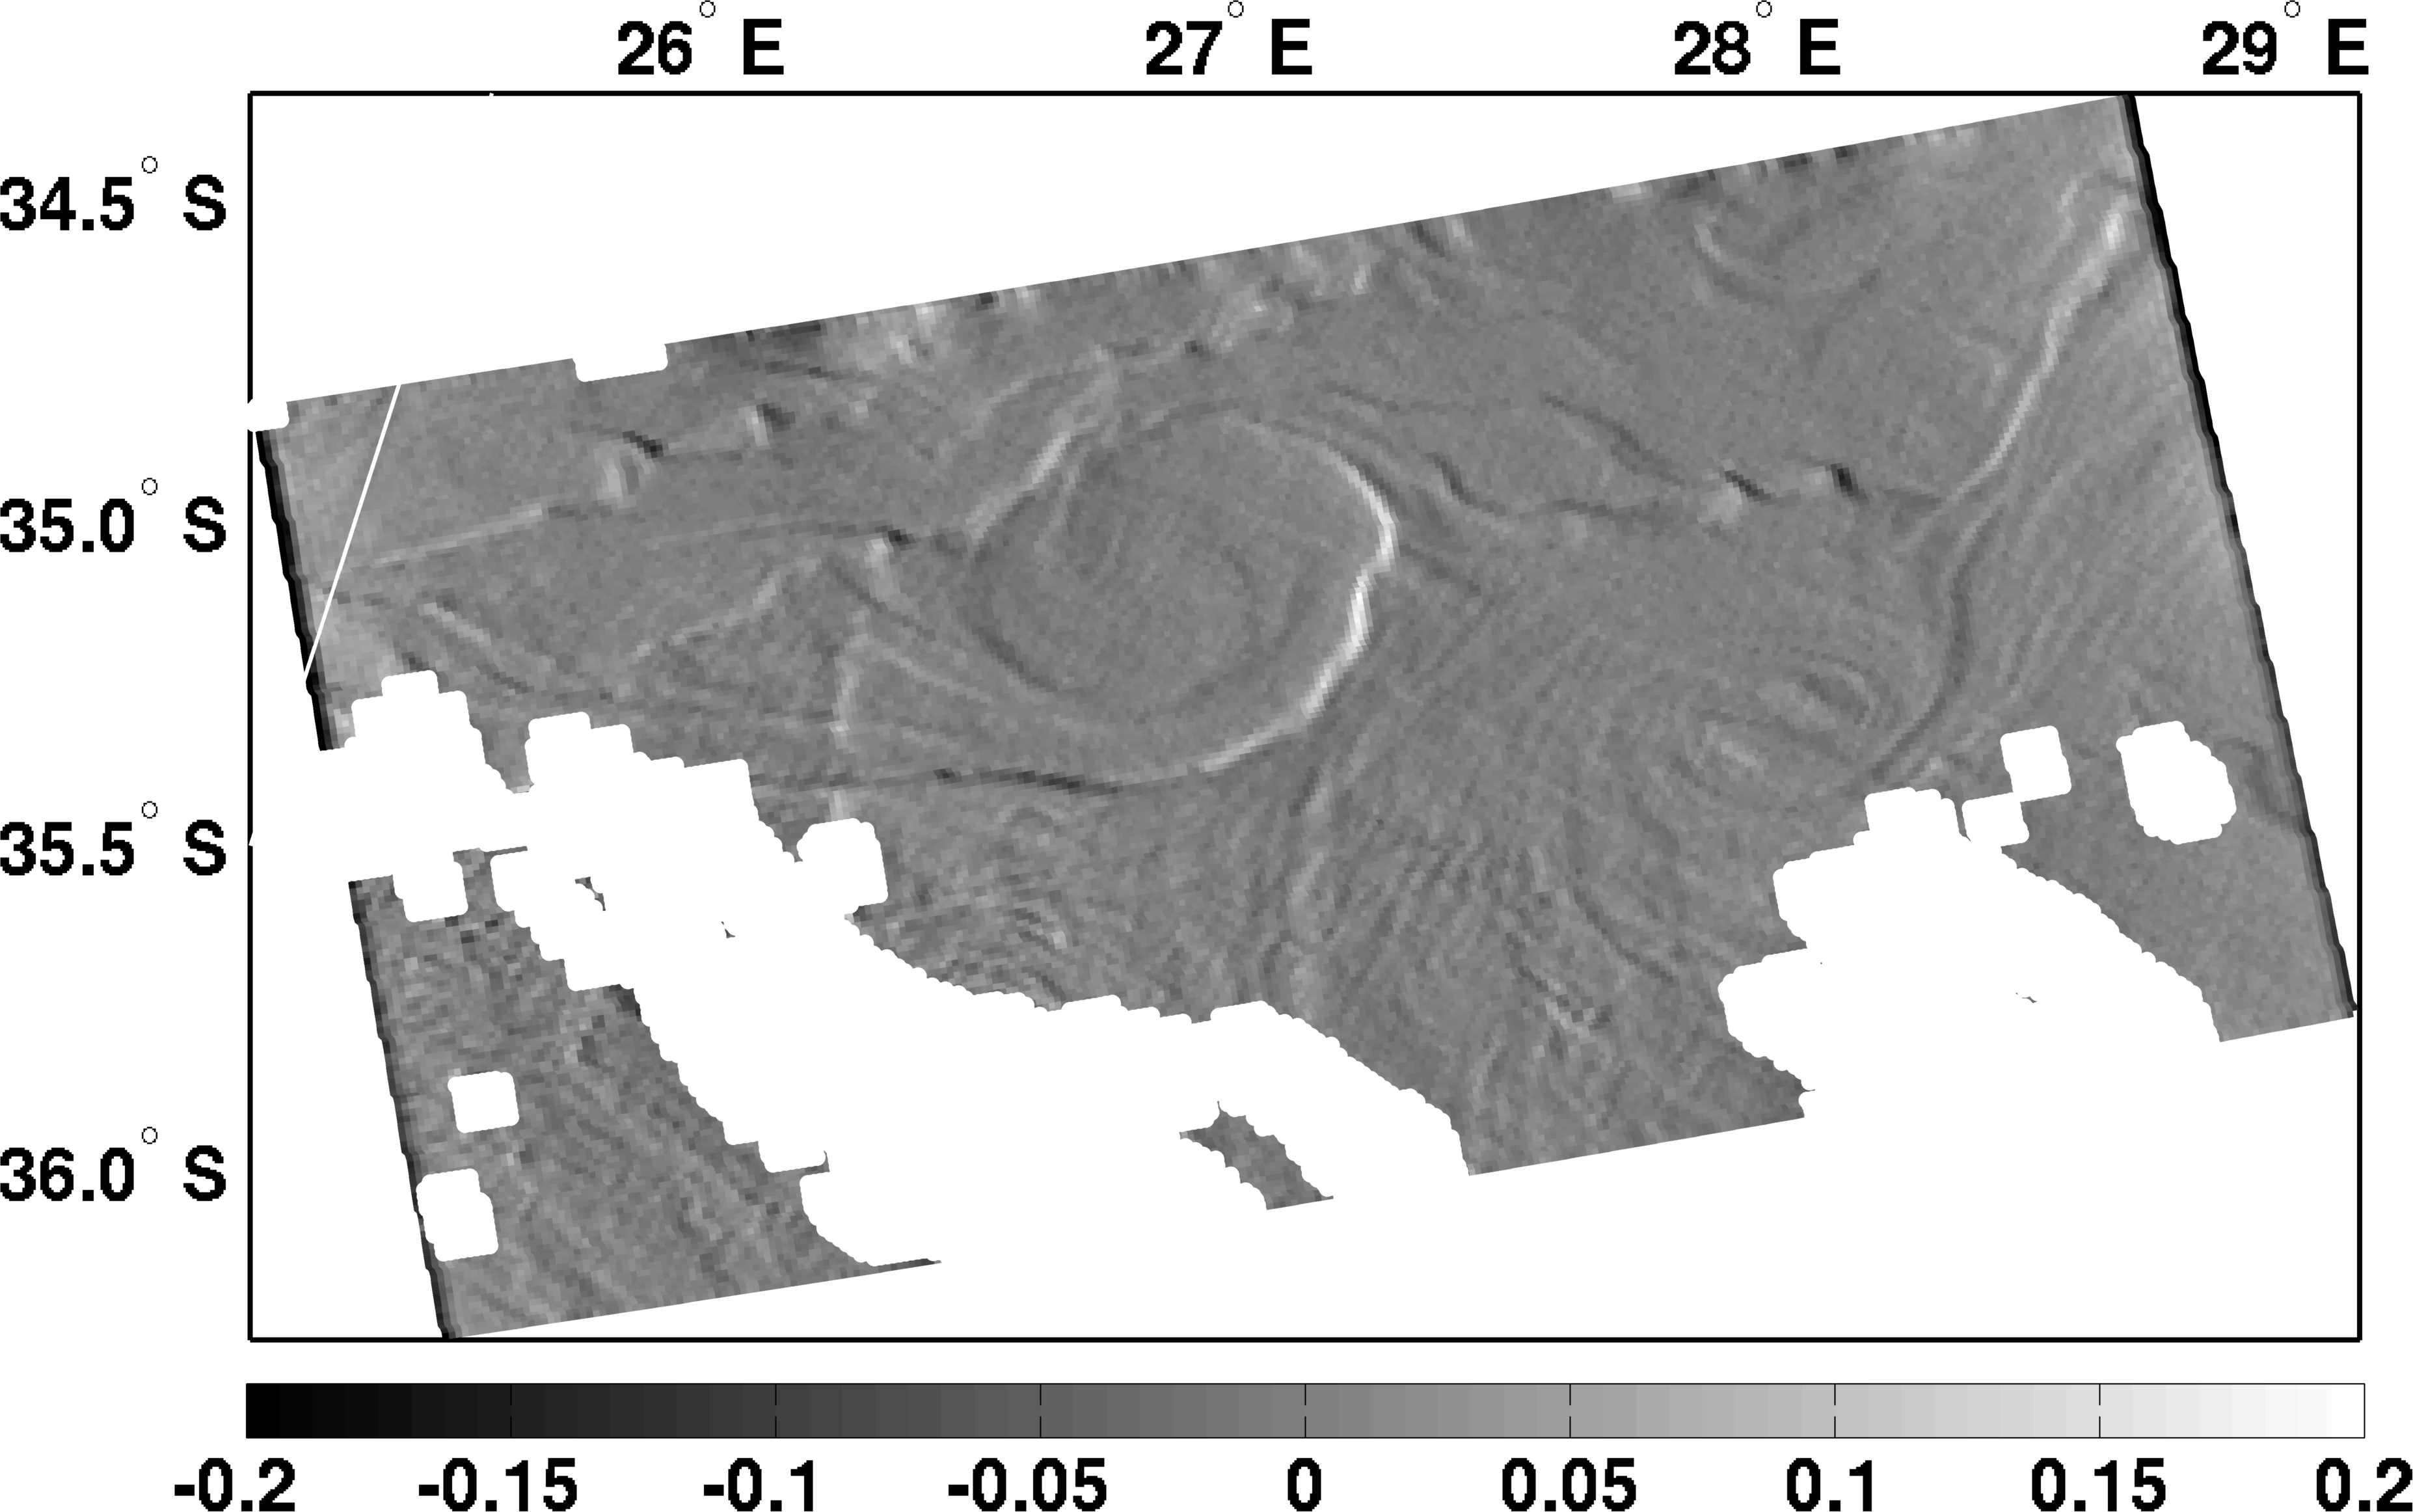
\includegraphics[width=1\linewidth]{fig3_11d}}
	\end{minipage}
    \\
    \floattitle{(а) Дивергенция поля поверхностного течения, полученное по полю ТПО (Рисунок~33~а). Яркие области на рисунке (а) соответствуют конвергенции течения, а тёмные -- дивергенции (детальнее см. подпись к Рисунку~\ref{fig:3.6b}). Другие рисунки -- симуляции RIM модели поверхностных проявлений грибовидной структуры, представленной в виде контрастов СКН (б), обрушения волн (в), и контрастов УЭПР (г)}
    \caption{Фрагменты восстановленного по ТПО поля дивергенции поверхностного течения и смоделированных характеристик: контрастов СКН, обрушений волн, и контрастов УЭПР}
    \label{fig:3.11}
\end{figure}


Сравнение численного моделирования RIM (приведённого на Рисунке~35) с упрощёнными выражениями в уравнениях \eqref{eq:1.5}, \eqref{eq:1.7}, \eqref{eq:1.8} и \eqref{eq:1.9} даёт возможность получить константу пропорциональности для дальнейшего использования упрощённых решений в практических целях. Мы пришли к следующим соотношениям:



\begin{equation} \label{eq:3.11)} \begin{array}{l} {\frac{\tilde{s}^{2} }{s^{2} } =-\frac{c_{s} }{u_{*}^{} (k_{c} K)^{1/2} } \nabla \cdot {\it u}} \\ {\frac{\tilde{q}_{} }{q_{0} } =-c_{q} \ln \left(\frac{u_{*} k_{b} }{g^{1/2} K^{1/2} } \right)\frac{g}{u_{*}^{2} k_{b} } \omega _{b}^{-1} \nabla \cdot {\it u}} \end{array} \end{equation} 



\noindent где $c_{s} =$ 180 и $c_{q} =$ 470 при $k_{c} =(g/\gamma )^{1/2} $ и $k_{b} =k_{R} /10$ ($\gamma $ - поверхностное натяжение, $k_{R} $ - волновое число радара).

В конечном счёте, анализ РСА и СКН сигнатур суб- и мезомасштабной динамики верхнего слоя океана отражает отчётливое текстурное сходство с полями конвергенции/дивергенции, хотя незначительные различия в контрастах паттернов всё же наблюдаются. Предположительно, причиной этому могут служить:

\begin{enumerate}
\item  несовершенное восстановление поверхностного течения и поля дивергенции по данным ТПО MODIS;

\item  неточности в поле локального ветра, ветровом дрейфе, Экмановском течении и оценках инерциальных течений;

\item  пространственно-временная эволюция мезомасштабных особенностей за пятичасовой интервал между съёмками ASAR и MODIS.
\end{enumerate}

Тем не менее, общее соответствие очень обнадёживает и прекрасно демонстрирует возможности для получения количественных оценок динамики верхнего слоя океана по мультисемнсорным поверхностным проявлениям мезомасштабных особенностей.



\newpage


\section{Выводы по главе} \label{sec:3.4}


Показано что блик является инструментом исследования динамики. Это продемонстрировано на примере ВВ. Известно что ВВ являются идеальным объектом для тестирования любого метода \dots \dots \dots .

Помимо течений, поверхностные проявления ВВ также хорошо видны в модуляциях уклонов морской поверхности. Это также связано с усилением СКН в зонах конвергенции течения ВВ, в то время как подавление наблюдается в зонах дивергенции. Эта связь между аномалиями СКН и дивергенцией поверхностного течения ВВ идентична модуляциям обрушений ветровых волн, вызванных ВВ, наблюдаемых Дуловым и др. в 1986 \citep{1986} в этом же районе исследования.



В отличии от ВВ, вопрос о возможности идентификации мезомасштабных течений остается открытым. В данной работе предлагается синергетический подход основанный на \dots \dots .

 

До сих пор численное понимание механизмов формирования РСА изображений шероховатости морской поверхности под воздействием полей дивергенции и конвергенции поверхностного течения было недостаточным. В данной главе предложен и применён новый синергетический подход для численного? анализа данных РСА и оптических спектрометров, включая инфракрасные каналы. НАДО ОБЪ\textbackslash ЯСНИТЬ В ЧЕМ ОН НОВЫЙ?

ИСХОДНЫМИ ЯВЛЯЕТСЯ КОМБИНАЦИЯ ПОЛЕЙ

- ТПО ПО ИК

-ЯРКОСТЬ В КРАСНОМ КАНАЛЕ

- УЭПР 



На основании которых делается вывод о реализуемости спутниковой диагностикеи 

Очевидно, что применённый синергетический подход ясно демонстрирует прекрасное соответствие аномалий СКН, реконструированных по изображению солнечного блика (сформированных полным спектром волн, от капиллярных до энергонесущих), с аномалиями шероховатости, восстановленных по РСА изображению. Далее обнаружено, что оба поля находятся в пространственном соответствии с фронтальными областями, представляющими градиенты ТПО. Поскольку типичная фронтальная область состоит из вдоль-фронтальной струи течения с интенсивной перекрестно-фронтальной динамикой и вертикальными движениями, мы ожидали получить именно эти результаты, на основании \citep{Kudryavtsev2005,Johannessen2005}.

- Основываясь на предположении, что циркуляция верхнего слоя океана квази двумерно, поле поверхностного квазигеострофического течения (КГТ) восстанавливается по снимку данных ТПО, следуя теории поверхностной квазигеострофической (ПКГ) динамики. 

- Поскольку результирующее поле КГТ является бездивергентным, его прямое взаимодействие с ветровыми волнами приводит к слабому проявлению на поверхности особенностей мезомасштабного течения, как уже было показано в \citep{Kudryavtsev2005,Johannessen2005}. Поэтому, скорее всего, механизм проявления несколько другой. 

- Взаимодействие вызванных ветром в верхнем слое потоков с полем КГТ (путём Экмановского адвективного механизма, и диабатического механизма перемешивания, как предложено в \citep{Klein1990,Garrett1981}  приводит к генерации достаточно сильного агеострофического течения, которое, в свою очередь, приводит к большим конвергенционным и дивергенционным поверхностным потокам, проявления которых мы и наблюдаем. В соответствии с предлагаемым предположением, интенсивная перекрестно-фронтальная динамика возникает как близ резких горизонтальных градиентов поля завихренности КГТ, так и в районе сильных вертикальных градиентов поля скорости КГТ.

- В соответствии с вышеизложенным, можно рассматривать наблюдаемое поразительное соответствие между аномалиями шероховатости и градиентами ТПО в качестве ``экспериментального подтверждения'' того факта, что влияние дивергенции поверхностного течения на короткие ветровые волны есть основной механизм, приводящий к поверхностным проявлениям мезомасштабных особенностей течения в виде аномалий ``шероховатости'' морской поверхности. 

- Помимо этого, стоит отметить, что корреляция между аномалиями шероховатости морской поверхности и модельной дивергенцией поверхностного течения наводит на мысль о надёжности модельного фреймворка для восстановления мезомасштабных поверхностных течений.

- Поле поверхностного течения, восстановленное по данным ТПО MODIS и ветру ASAR, также использовались в качестве входных параметров модели формирования РЛ-изображения RIM, для симулирования РСА УЭПР и СКН сигнатур. Реконструированное поле чётко отражает, что наблюдаемые аномалии на изображении РСА, вместе с аномалиями поля СКН, восстановленного по данным MODIS, представляют поверхностные проявления зон конвергенции и дивергенции океанического течения вдоль меандрирующих фронтов и вихрей.



В РЕЗУЛЬТАТЕ РЕАЛИЗАЦИИ ПОДЛХОДА ПОЯВЛЯЮТСЯ ПОЛЯ



- ГЕОСТРОФИКИ

- ПОЛЯ РСА-ВЕТРА

- ПОЛНЫЕ ПОЛЯ ТЕЧЕНИЙ ГЕОСТРОФИКА+ ВЕТРОВОЙ ДРЕЙФ + АГЕОСТРОФИЧЕСКАЯ 

- ПОЛЯ ДИВЕРГЕНЦИИ ТЕЧЕНИЙ

- ПОЛЯ ЩЕРОХОВАТОСТИ (В ЧАСТНОСТИ мсс) КОТОРЫЕ МОГУТ БЫТЬ ИСПОЛЬЗОВАНЫ В ДРУГИХ ПРИЛОЖЕНИЯХ

Т.е. в целом, в результате реализации подхода появляется новое качество. 

Подытоживая, можно утверждать, что предложенный синергетический подход, объединяющий ТПО, яркость солнечного блика и данные РСА, дополненный и другими источниками других данных более низкого разрешения (например, альтиметров и скаттерометров), предоставляет согласующееся численное решение положения и интенсивности зон конвергенции/дивергенции (апвеллинга/даунвеллинга) поверхностного течения. А это, в свою очередь, важный и многообещающий шаг в сторону прогресса численной интерпретации и понимания динамики верхнего слоя океана по двумерным изображениям его поверхностных проявлений.



\clearpage